\documentclass[12pt,a4paper]{article}

\usepackage{hyperref}
\usepackage{graphicx}
\usepackage{float}
\usepackage{relsize}
\usepackage{amsmath}
\usepackage{subfigure}
\usepackage{fancyhdr}
\usepackage[font=scriptsize]{caption}

\usepackage{geometry}
\geometry{
 a4paper,
 total={170mm,257mm},
 left=20mm,
 top=20mm,
}

\usepackage{xepersian}
\settextfont[Scale=1.2]{B Nazanin}
%\fontsize{14}{20}\selectfont
\linespread{1.5}
%%%%%%%%%%%%%%%%%%%%%%%%%%%%%%%%%%%%%%%%%%%%%%%%%%%%%%%%%%%%%%%%%%%%%%%%%%
%\includeonly{introduction}
%\includeonly{sceneUnderstanding}

%%%%%%%%%%%%%%%%%%%%%%%%%%%%%%%%%%%%%%%%%%%%%%%%%%%%%%%%%%%%%%%%%%%%%%%%%%
\newcommand\numberthis{\addtocounter{equation}{1}\tag{\theequation}}

\newcommand{\enfootnote}[1]{\LTRfootnote{\lr{#1}}}

\newcounter{mypagecount}% create a new counter
\setcounter{mypagecount}{0}% set it to something just in case
\newenvironment{interlude}{% create a new environment for the unnumbered section(s)
\newgeometry{top=50mm}
  \clearpage
%  \setcounter{mypagecount}{\value{page}}% use the new counter we created to hold the page count at the start of the unnumbered section
  \thispagestyle{empty}% we want this page to be empty (adjust to use a modified page style)
  \pagestyle{empty}% use the same style for subsequent pages in the unnumbered section
  }{%
  \clearpage
%  \setcounter{page}{\value{mypagecount}}% restore the incremented value to the official tally of pages so the page numbering continues correctly
\newgeometry{top=20mm}

  }


\newcommand{\createTitlePage}[2]{
\newpage
\begin{interlude}
\vspace{5cm}
\section[#1 #2]{
    \Huge
    \textbf{#1}\\
    \center
    \textbf{#2}
    }
    
\end{interlude}

\newpage
}

\newcommand{\ML}[1]{\mathlarger{\mathlarger{#1}}}

\SepMark{-}

 \makeatletter
    \renewcommand\tableofcontents{%
        \section*{\centering\contentsname
            \@mkboth{%
               \MakeUppercase\contentsname}{\MakeUppercase\contentsname}}%
        \@starttoc{toc}%
        }
     \renewcommand\listoftables{%
            \section*{\centering\listtablename}%
              \@mkboth{%
                  \MakeUppercase\listtablename}%
                 {\MakeUppercase\listtablename}%
            \@starttoc{lot}%
            }
    \renewcommand\listoffigures{%
        \section*{\centering\listfigurename}%
          \@mkboth{\MakeUppercase\listfigurename}%
                  {\MakeUppercase\listfigurename}%
        \@starttoc{lof}%
        }
\makeatother
%%%%%%%%%%%%%%%%%%%%%%%%%%%%%%%%%%%%%%%%%%%%%%%%%%%%%%%%%%%%%%%%%%%%%%%%%%
\begin{document}

%\pagestyle{fancy}
%\renewcommand{\sectionmark}[1]{\markright{\thesection\ #1}}
%\renewcommand{\subsubsectionmark}[1]{\markright{\thesection\ #1}}
%\rhead{\fancyplain{}{\rightmark }} % 1. sectionname, 1.1 subsection name etc
%%\cfoot{\fancyplain{}{\thepage}}

\pagenumbering{alph}
\thispagestyle{empty}
%\begin{figure}[h]
%\center
%\includegraphics[scale=0.08]{{Imgs/fa_aut_with_name.png}}
%\end{figure}

%\begin{center}
%\LARGE{دانشکده مهندسی کامپیوتر و فن‌آوری اطلاعات\\ دانشگاه صنعتی امیرکبیر}
%\end{center}

\begin{center}
\large{درس سمینار رشته هوش مصنوعی}
\end{center}


\begin{center}

\LARGE{\textbf{
تولید خودکار شرح بر تصاویر با استفاده از شبکه‌های عصبی کانولوشنی عمیق و بازگشتی
}}
\\
\vspace{5mm}
\small{
\lr{
Automatic Image Captioning Using Deep Convolutional and Recurrent Neural Networks
}}

\vspace{2cm}
\Large{
\textbf{
استاد راهنما}
\\}
\vspace{2mm}
\large{
 دکتر صفابخش
}
\\
\vspace{1cm}
\Large{
\textbf{پژوهش‌گر}
\\
\vspace{2mm}
\large{
احمد اسدی\\
۹۴۱۳۱۰۹۱
}
}
\end{center}

\begin{center}
%
%
%\vspace{2cm}
% موعد تحویل: بیست و چهارم اردیبهشت‌ماه
\vfill
اردیبهشت‌ماه ۱۳۹۵
\end{center}


\newpage
\vfill
\begin{center}
\textbf{چکیده}
\end{center}
‫با توجه به افزایش چشم‌گیر تعداد تصاویر مورد استفاده کاربران در فضاهای مجازی و همین‌طور با در نظر گرفتن گرایش روزافزون کاربران به ذخیره‌سازی تصاویر در رایانه‌های شخصی، مساله مدیریت این تصاویر و یافتن تصاویر خاص بین مجموعه تصاویر موجود، به یکی از مسائل مهم و پرکاربرد در زمینه بینایی ماشین تبدیل شده‌ است. گام اساسی در این راستا، دست‌یابی به سامانه‌ای است که قادر به تولید خودکار شرح برای تصاویر باشد. شرح این تصاویر که در قالب جملات زبان طبیعی ارائه می­شود باید علاوه بر سازگاری با موضوع تصویر و توصیف صحیح صحنه، به لحاظ دستور زبان و معنا صحیح و کامل باشد. 
\newpage
\tableofcontents
\newpage
\listoffigures
\newpage
\listoftables


\newpage
\pagenumbering{arabic}

%\createTitlePage{فصل اول}{مقدمه}
\createTitlePage{فصل اول}{مقدمات}
\subsection{مقدمه}

به دنبال پیشرفت تکنولوژی در ساخت دوربین‌های عکاسی و ورود دوربین‌های نیمه‌خودکار و خودکار به بازار، تعداد زیادی از کاربران سیستم‌های رایانه‌ای به استفاده از این تکنولوژی در ثبت تصاویر مورد علاقه خود جذب شده‌اند. دقت و کیفیت مطلوب تصویربرداری از یک سو و سهولت استفاده از دوربین‌ از سوی دیگر، باعث شده‌اند تعداد تصاویر ثبت شده توسط کاربران به طور روزافزون افزایش یابد؛ به‌طوری‌که امروزه اغلب کاربران، تعداد بی‌شماری از این تصاویر را در گوشی‌های تلفن همراه، تبلت‌ها و رایانه‌های شخصی خود نگه‌داری می‌کنند.
از جمله مشکلاتی که در اثر ایجاد این حجم وسیع از تصاویر بوجود آمده، مشکل مدیریت این تصاویر و یافتن تصاویر خاص بین مجموعه بزرگی از تصاویر موجود، است.
\\
برای دست‌یابی به سامانه‌ای که بتواند تعداد زیادی از تصاویر موجود را مدیریت نماید، ابتدا باید صحنه موجود در تصویر را به درستی درک کرد. درک صحیح از صحنه، عبارت است از بیان تصویر به نحوی که اطلاعات کلی موجود و هدف اصلی تصویر، واضح و مشخص باشد. این بیان می‌تواند شامل اجسام موجود در تصویر، رابطه مکانی بین اجسام، فعالیت به تصویر کشیده شده، شرایط محیطی موثر بر صحنه و مواردی از این دست باشد. از طرفی باید به نحوی محتوای تصاویر را بیان کرد که بتوان عملیات جستجو را بر اساس مدل بیان شده تصاویر انجام داد. در این‌صورت به‌ازای هر تصویر، یک نمونه از مدل مطابق با تصویر ایجاد و ذخیره خواهد شد. پرس‌و‌جوی\enfootnote{Query} کاربر به فضای مدل، نگاشت شده و تصویر معادل با مدلِ استخراج شده، به عنوان نتیجه جستجو نمایش داده می‌شود. علاوه بر این، مساله مدیریت تصاویر، به مساله مدیریت مدل‌های موجود کاهش داده می‌شود.
\\
تولید شرح کلی بر تصاویر\enfootnote{Holistic Image Caption}، بیان مناسبی از صحنه موجود در تصویر را ارائه می‌دهد. شرح تولید شده بر تصاویر، در قالب مجموعه‌ای از جملات زبان طبیعی\enfootnote{Natural Language Sentences} ارائه‌ می‌شود که عموما بیان‌گر اجسام موجود در صحنه‌، ارتباطات مکانی بین اجسام و اطلاعات مشخص دیگر است که در هر پژوهش می‌تواند متفاوت باشد. بنابراین، دست‌یابی به سامانه‌ای که قادر به تولید خودکار شرح کلی بر تصاویر باشد، اساسی‌ترین گام در راستای تولید نرم‌افزارهای مدیریت تصاویر است.
\\
یکی از اولین ایده‌های مطرح شده در این زمینه، با الهام از پژوهش­‌های صورت گرفته در زمینه ترجمه ماشین\enfootnote{Machine Translation}
 به‌وجود آمده‌ است که با هدف ترجمه جملات یک زبان به زبان دیگر به طور خودکار، انجام شده‌اند. در این راستا، یک جمله از زبان مبدا\enfootnote{Source Language}، با روش‌های مختلف، تبدیل به یک بردار ویژگی\enfootnote{Feature Vector} می‌شود که مشخصه‌های اصلی جمله اولیه را نمایش می‌دهد. سپس بردار ویژگی حاصل، با اعمال روش­‌های گوناگون دیگری، تبدیل به یک جمله از زبان مقصد\enfootnote{Destination Language} می­گردد که در آن تمام ویژگی‌های موجود در بردار ویژگی بیان شده‌‌اند.
با توجه به فرایند مذکور، اگر به جای جمله زبان مبدا، یک تصویر به بردار ویژگی تبدیل شده و سپس با استفاده از روش‌های موجود قبلی، بردار ویژگی حاصل به جمله زبان مقصد ترجمه شود، جمله‌ای معادل با تصویر ورودی به‌دست خواهد آمد  که بیان‌گر محتوای به تصویر کشیده شده در تصویر ورودی است\cite{xu2015show}.
\\
شرح خودکار تصاویر، توجه پژوهش‌گران بسیار زیادی را به خود جلب کرده است و فعالیت‌های متنوع و متعددی در این راستا انجام شده‌اند. علی‌رغم وجود پژوهش‌‌های فراوان و متفاوت، می‌توان یک بستر کلی برای تمام فعالیت‌های موجود در این زمینه ارائه داد. بر این مبنا، فرایند کلی که در عموم پژوهش‌های انجام‌شده، پی گرفته شده‌است، از دو بخش اساسی تشکیل می‌شود.
\begin{enumerate}
\item بازنمایی تصاویر، با استفاده از بردار ویژگی
\item تبدیل بردار ويژگی به‌دست‌آمده به جملات صحیح زبانی
\end{enumerate}


\subsection{تعریف مساله}
در این پروژه قصد داریم سامانه‌ای ارائه دهیم که قادر به تولید شرح کوتاه بر تصاویر باشد. دو دیدگاه اساسی در دست‌یابی به چنین سامانه‌ای مطرح است.
\begin{enumerate}
\item
 یافتن نقاط توجه\enfootnote{Attention Points} 
در تصاویر و تولید جملات توصیف‌کننده اجسام مستقر در این نقاط به طوری‌که توصیف جسم مستقر در نقطه توجه و اجسام مرتبط با آن در جملات تولیدی، وجود داشته باشد.
\item  تولید شرح جامع بر تصاویر به طوری‌که تمام اجسام موجود در صحنه به همراه روابط موجود بین آن‌ها توصیف شوند. 
\end{enumerate}

شرح کوتاه تولید شده در این پروژه، به معنی تولید جملاتی است که مستقیما به توصیف صحنه، اجسام موجود در صحنه و روابط بین آن­ها می­پردازند.
به طور کلی، دو چالش عمده در این پژوهش مورد توجه قرار خواهد گرفت:
\begin{enumerate}
\item  توصیف صحنه باید دقیق باشد؛ به این معنی که اجسام موجود در صحنه باید به طور دقیق از هم تفکیک شده و دسته‌بندی شوند. تصویر توصیف شده باید در قالب مناسبی بازنمایی شود که بتوان به راحتی از آن برای تولید جمله استفاده نمود.
\item  جملات تولید شده برای شرح تصویر باید به لحاظ دستور زبان، املا و معنا صحیح بوده و با تصویر مرتبط خود سازگار باشند و آن را به درستی و دقت شرح دهند.
\end{enumerate}

\subsection{درک صحنه}
مساله درک صحنه، یکی از چالش‌های بزرگ و قدیمی مطرح در زمینه بینایی ماشین است. در گذشته، هدف اغلب پژوهش‌گران از طرح این مساله، توصیف صحنه موجود در تصویر با دیدن لحظه‌ای تصویر بوده است؛ اگر‌چه امروزه، تعریف این مساله دچار تغییر شده است.
\\
به‌طور کل نمی‌توان تعریف جامع و شاملی برای درک صحنه ارائه داد. اگرچه تعاریفی عمومی ارائه شده‌اند که کلیات این مفهوم را توضیح می‌دهند. پژوهش‌‌گران در این زمینه هریک سعی در ارائه تعریفی برای این مفهوم دارند که برای کاربرد مورد نظر خود کافی و مفید باشد. به عنوان مثال، یکی از جدیدترین تعاریف برای درک صحنه در پژوهش\cite{hoiem2015guest} ارائه شده است:

\begin{enumerate}
\item [*]
«توانایی تحلیل بصری یک صحنه برای پاسخ‌دادن به سوالاتی مانند سوالات زیر:
\begin{itemize}
\item[-] چه اتفاقی در حال رخ دادن است؟
\item[-] چرا این اتفاق در حال رخ دادن است؟
\item[-] اتفاق بعدی که رخ خواهد داد، چیست؟»
\end{itemize}

\end{enumerate}

به طور کل می‌توان درک صحنه را چنین معنا کرد:
\\
\begin{enumerate}
\item [*]
درک صحنه، فرایندی است که طی آن، یک سامانه رایانه‌ای با استفاده از الگوریتم‌های موجود، اطلاعات بصری نهفته در تصاویر را استخراج کرده و در قالب مناسبی بازنمایی\enfootnote{Representation} کند به طوری‌که این اطلاعات برای توصیف صحنه کافی و مفید باشد.
\end{enumerate}

با این تعریف، اگر چه مفهوم درک صحنه کمی روشن می‌شود اما نکات مبهمی مانند این‌که چه نوع اطلاعاتی از تصویر استخراج شود، نیاز به توضیح و تفسیر بیشتری دارند. در تمام پژوهش‌های موجود در زمینه درک صحنه، که تعدادی از آن‌ها را در فصل بعدی مورد بررسی قرار خواهیم داد، تعریف اتخاذ شده برای درک صحنه، همین تعریف است با این تفاوت که اطلاعات مورد نیاز برای استخراج، در هر پژوهش، بسته به کاربرد تعریف می‌شود.
\\
موارد مختلفی که به عنوان اطلاعات لازم برای درک و توصیف صحنه، در پژوهش‌ها به چشم می‌خورد عموما شامل موارد زیر هستند:

\begin{enumerate}
\item دسته‌ صحنه\enfootnote{Scence Class} (دریا، جنگل، خیابان، کلاس درس و مواردی از این دست)
\item دسته‌ اجسام\enfootnote{Object Class} موجود در صحنه (صندلی، مرد، گربه و مواردی از این دست)
\item ارتباط مکانی بین اجسام موجود (بالا، کنار، پشت و مواردی از این دست)
\item رخدادی\enfootnote{Event} که در صحنه در حال اتفاق است (مانند نشستن، دویدن، کارکردن و مواردی از این دست)
\end{enumerate}

\subsubsection{پژوهش‌های انجام‌شده در زمینه درک صحنه توسط مغز انسان}
مساله درک صحنه، مانند بیشتر مسائل موجود در زمینه بینایی ماشین، الهام گرفته از نحوه رفتار انسان‌ها است. اغلب انسان‌ها با دیدن یک تصویر قادرند توصیف کامل و دقیقی از آن تصویر ارائه دهند که شامل تمام نکات لازم و ضروری نهفته در تصویر باشد. در بیشتر موارد، زمان مورد نیاز برای مغز انسان به منظور پردازش یک تصویر و توصیف آن، زمان بسیار کم و ناچیزی است. این مطلب، این ایده را در ذهن تداعی می‌کند که بخش قابل توجهی از اطلاعات مورد نیاز از هر تصویر، در اولین لحظاتی که تصویر به مغز می‌رسد (در نگاه اول) قابل استخراج است. بنابراین سامانه‌های رایانه‌ای باید قادر باشند با الگو گرفتن از مغز انسان، در کوتاه‌ترین زمان ممکن، اطلاعات کافی و مفید نهفته در تصویر را استخراج کرده و صحنه به نمایش کشیده شده در تصویر را توصیف کنند.
\\
این فرض که مغز انسان می‌تواند در کوتاه‌ترین زمان ممکن، بیشترین حجم اطلاعات تصویر را به درستی استخراج نماید، توسط پژوهش‌گران متعددی مورد ارزیابی قرار گرفته است. از جمله اولین پژوهش‌هایی که به بررسی این فرض پرداخته‌اند می‌توان به 
\cite{potter1976short}
و
\cite{potter2002recognition}
اشاره کرد. در این‌ پژوهش‌ها، با نشان دادن تصاویر به صورت دنباله‌ای\enfootnote{Image Series} به مجموعه‌ای از افراد، از آن‌ها خواسته شده تا بهترین و دقیق‌ترین توصیفی را که می‌توانند، برای تصاویری که دیده‌اند، بازگو کنند. در این دو پژوهش نتیجه گرفته شده است که انسان می‌تواند یک تصویر معمولی را در بازه زمانی کمتر از ۲۰۰ میلی‌ثانیه، تشخیص داده و آن را توصیف کند. اگرچه این زمان برای تشخیص و توصیف یک تصویر کافیست، زمان مورد نیاز برای به‌خاطرسپاری تصویر بسیار بیشتر از این مقدار است.
\\
در پژوهش\cite{fei2007we}
آزمایش دیگری انجام شده که از اهمیت بسیاری برخوردار است. در پژوهش‌های قبلی، افرادی که تصاویر را توصیف می‌کردند، درباره موضوع کلی تصاویر اطلاعاتی داشتند. اما در این آزمایش، تصاویر مختلفی از دنیای واقعی که محدود به شرایط خاصی نبوده‌اند، بدون ارائه پیش‌فرض درباره موضوع، به افراد نمایش داده شده و از آن‌ها خواسته شده که تصویر را به بهترین شکل توصیف کنند. آزمایشات در این پژوهش، در دو مرحله انجام شده‌اند.
\begin{enumerate}
\item توسط یک رایانه، تصاویر متعددی در بازه‌های زمانی متفاوت به افراد نمایش داده می‌شوند و پس از اتمام زمان نمایش هر تصویر، یک ماسک بصری، تصویر را می‌پوشاند. در این حالت از افراد خواسته‌شده  است که بهترین توصیف ممکن از تصویر را تایپ کنند. شرایط محیطی آزمایشات مطابق با استانداردها رعایت شده است. هر تصویر به طور تصادفی بین 27 الی 500 میلی ثانیه روی نمایش‌گر نمایش‌داده شده و سپس یک ماسک روی تصویرقرار گرفته و افراد فرصت دارند تا توصیف خود را از تصویر، بنویسند.


\begin{figure}[H]
\center
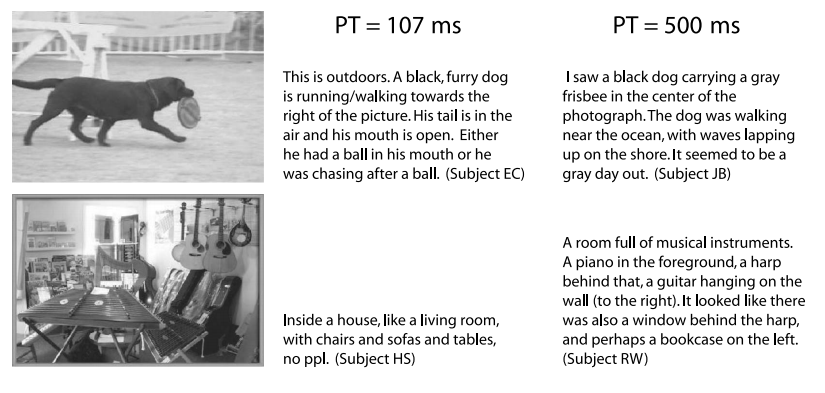
\includegraphics[scale=0.5]{./Imgs/fei2007we_res2.png}
\caption[نمونه توصیف‌های افراد برای تصاویر]{نمونه‌ توصیف‌های افراد برای تصاویر\cite{fei2007we}}
\label{fig:f2007we1}
\end{figure}



\item در این مرحله، آزمایش روی افراد متفاوتی انجام شده‌است. این گروه افراد موظفند پس از دیدن تصاویر، به بهترین شکل ممکن آن‌ها را دسته‌بندی کنند. برخلاف افراد شرکت‌کننده در آزمایش قبلی  که می‌توانستند به هر شکلی اطلاعات استخراج شده را بنویسند، به افراد حاضر در این گروه یک فرم مشخص از دسته‌اطلاعات مطلوب داده شده است که افراد موظفند آن را براساس محتوای تصویری که دیده‌اند، پر کنند. شکل\ref{fig:f2007we2}
ساختار مطلوب پاسخ افراد را در این آزمایش نمایش می‌دهد.

\begin{figure}[H]
\center
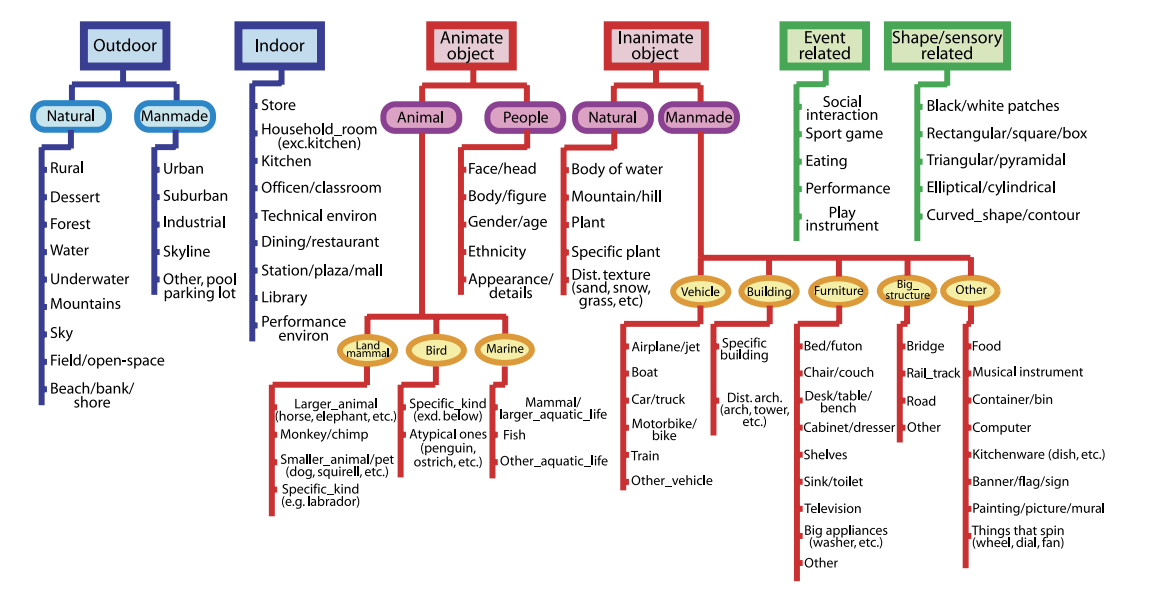
\includegraphics[scale=0.4]{./Imgs/fei2007we_exp1.png}
\caption{ساختار مطلوب اطلاعات استخراج‌شده از تصاویر\cite{fei2007we}}
\label{fig:f2007we2}
\end{figure}

این ساختار با تحلیل پاسخ‌های جمع‌آوری شده از آزمایش اول استخراج شده است و شامل انواع مختلفی از اطلاعات است که افراد در آزمایش اول به آن اشاره‌کرده‌اند.





\end{enumerate}


شکل\ref{fig:f2007wd}
چند نمونه از تصاویر مورد استفاده در آزمایشات این پژوهش را نمایش می‌دهد. این تصاویر از اینترنت استخراج شده‌اند. برای استخراج این تصاویر از فضای اینترنت، از یک گروه افراد شامل ۱۰ نفر که با موضوع پژوهش آشنا نبوده‌اند خواسته‌شده تا هر یک، نام ۵ دسته صحنه مختلف را به طور تصادفی بنویسند. پس از حذف نام‌های تکراری، ۲۵ الی ۳۰ نام منحصربه‌فرد باقی مانده‌است. سپس تصاویر مربوط به هریک از این نام‌ها توسط موتور جستجوی گوگل استخراج شده و ۳ الی ۶ تصویر از صفحات اولیه نتایج به عنوان تصاویر نمونه انتخاب شده‌اند.

\begin{figure}[H]
\centering
	\subfigure[چند نمونه از تصاویر در محیط باز]{
		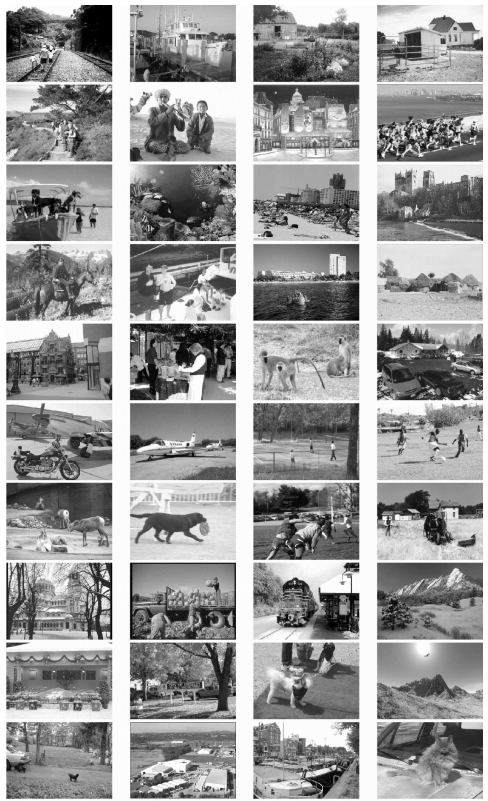
\includegraphics[scale=0.4]{./Imgs/fei2007we_data1.png}
	}	
	\hspace*{1mm}
	\subfigure[چند نمونه از تصاویر در محیط بسته]{
		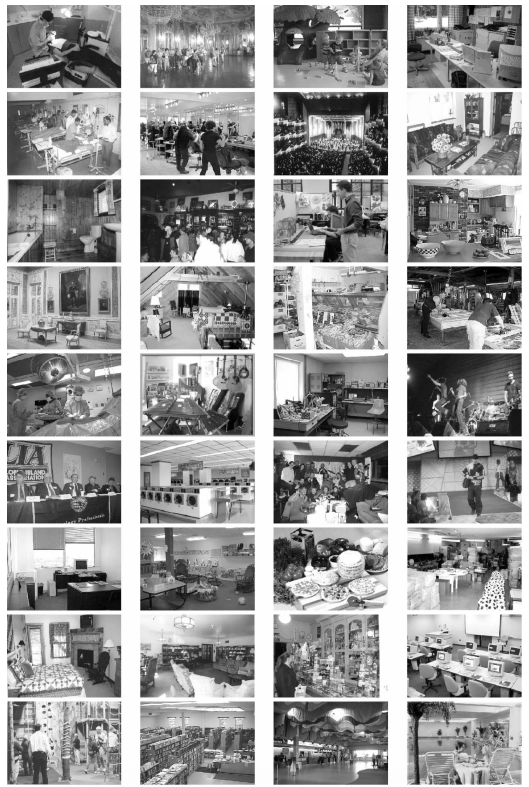
\includegraphics[scale=0.4]{./Imgs/fei2007we_data2.png}
	}
\caption{تصاویر دنیای واقعی مورد استفاده در آزمایشات\cite{fei2007we}}
\label{fig:f2007wd}
\end{figure}


ارزشمندترین نکته درباره پژوهش انجام‌شده، یافته‌های آن است. این پژوهش نکاتی را در مورد توانایی مغز انسان در توصیف صحنه روشن می‌کند که حائز اهمیت هستند. در ادامه این نتایج را بررسی خواهیم کرد.
\subsubsection{نتایج به‌دست‌ آمده از آزمایشات}
\begin{enumerate}
\item
حداکثر زمان لازم برای مغز انسان به منظور درک صحنه، برابر با 500 میلی‌ثانیه است.
\item
این مدت زمان، برای صحنه‌های ساده‌ و بدون پیچیدگی، به حدود ۱۰۰ میلی‌ثانیه می‌رسد. به عنوان نمونه در شکل\ref{fig:f2007we1} تصویر اول که دارای پیچیدگی‌های کمتری نسبت به تصویر دوم است در مدت زمان ۱۰۷ میلی‌ثانیه، به‌طور کامل توصیف شده‌است در صورتی‌که تصویر دوم که به نسبت، پیچیده‌تر است، مدت‌زمان بیشتری برای توصیف نیاز داشته‌است.
\item
با استفاده از ساختارمندسازی پاسخ‌های افراد در آزمایش دوم و اطلاعات جمع‌آوری شده در درخت پاسخ‌ها (که در شکل\ref{fig:f2007we2} نمایش‌ داده شده است) و میانگین‌گیری روی تمام تصاویر، نمودارهای مقایسه‌ای برای مدت زمان 107 میلی‌ثانیه و 500 میلی‌ثانیه ایجاد شده‌ است. شکل\ref{fig:f2007res3}
نمودارهای مقایسه‌ای را نمایش‌ می‌دهد. در این نمودارها، میله‌های قرمز نشان‌دهنده نتایج برای زمان ۵۰۰ میلی‌ثانیه و میله‌های آبی نمایش‌دهنده نتایج برای حالت ۱۰۷ میلی‌ثانیه هستند.
در دو نمودار اول (نمودارهای بالا سمت راست و بالا سمت چپ) تشخیص و استخراج اطلاعات مربوط به اجسام مختلف بسته به متحرک بودن\enfootnote{Animated} یا متحرک نبودن\enfootnote{Inanimated} آن‌ها، در نمودار سوم (نمودار پایین سمت چپ) تشخیص و استخراج اطلاعات مربوط به صحنه موجود در تصویر و در نمودار چهارم‌ (نمودار پایین سمت راست) تشخیص و استخراج اطلاعات مربوط به رخداد موجود در تصویر، مورد بررسی قرار گرفته‌اند.


\begin{figure}[H]
\center
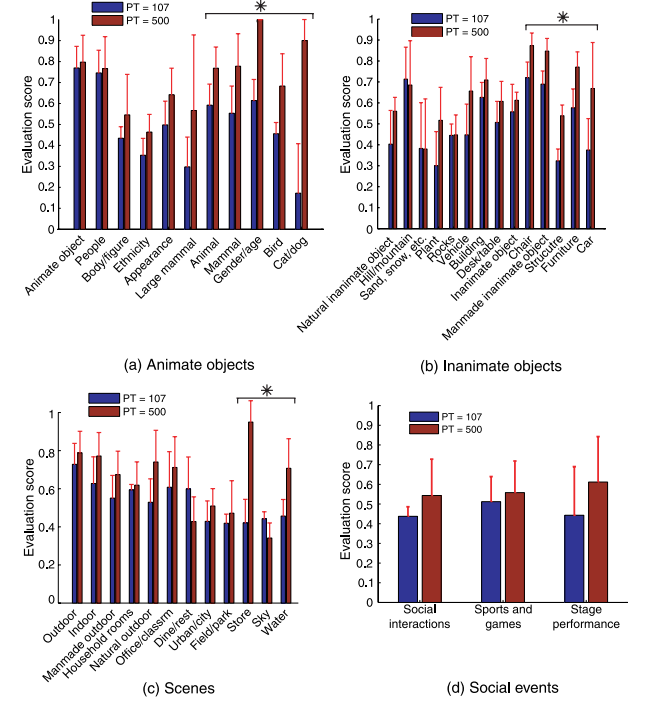
\includegraphics[scale=0.6]{./Imgs/fei2007we_res3.png}
\caption[نمودار مقایسه‌ای عملکرد مغز در درک صحنه]{نمودارهای مقایسه‌ای عملکرد مغز انسان در درک صحنه در بازه‌های زمانی ۱۰۷ و ۵۰۰ میلی‌ثانیه\cite{fei2007we}}
\label{fig:f2007res3}
\end{figure}

همان‌طور که مشخص است، مدت زمان ۱۰۷ میلی‌ثانیه برای مغز انسان، زمان بهینه برای توصیف صحنه است. تفاوت‌های بین نتایج در اکثر موارد، جزئی و در مقابل تفاوت زمانی موجود، بسیار کوچک هستند.
به علاوه، در تمام مواردی که نیاز به اطلاعات کلی از تصویر وجود دارد، تفاوت بین دو بازه زمانی چندان چشم‌گیر نیست، اما در مواردی که برای تشخیص نیاز به دانستن جزئیات بیشتر از تصویر وجود دارد (مانند سن، جنسیت و نوع حیوان) تفاوت بین دو زمان، قابل ملاحظه است.
\\
همین‌طور با مقایسه تفاوت عملکرد بین حالات متحرک بودن و متحرک نبودن اجسام، فواصل موجود در نمودارها قابل ملاحظه می‌شود. در حالت کلی، تفاوت بین عملکرد مغز در دو بازه، در حالتی‌که اجسام ساکن در تصویر وجود دارند به مراتب کمتر از حالتی است که اجسام موجود در تصویر، متحرک باشند.
\end{enumerate}

شکل\ref{fig:f2007res4} نمونه دیگری از نتایج به‌دست‌آمده از آزمایشات را در مدت‌زمان‌های مختلف نمایش ‌می‌دهد.



\begin{figure}[H]
\center
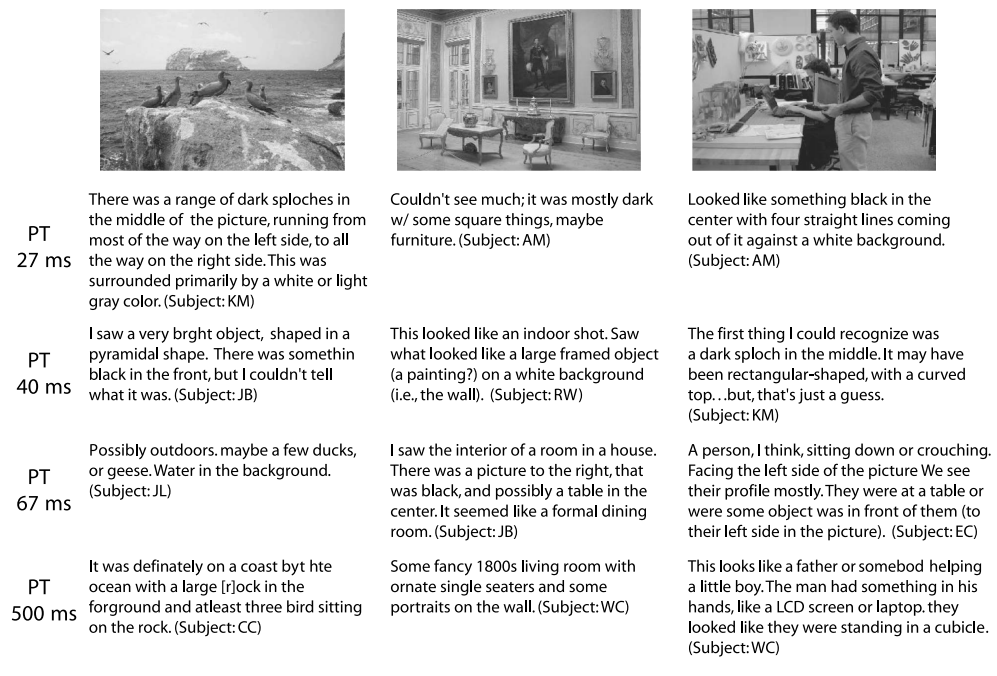
\includegraphics[scale=0.4]{./Imgs/fei2007we_res4.png}
\caption{نمونه‌ای از نتایج به‌دست‌آمده از آزمایشات\cite{fei2007we}}
\label{fig:f2007res4}
\end{figure}
%%%%%%%%%%%%%%%%%%%%%%%%%%%%%%%%%5

\subsection{جمع‌بندی}
‫با توجه به افزایش چشم‌گیر تعداد تصاویر مورد استفاده کاربران در فضاهای مجازی و همین‌طور با در نظر گرفتن گرایش روزافزون کاربران به ذخیره‌سازی تصاویر در رایانه‌های شخصی، مساله مدیریت این تصاویر و یافتن تصاویر خاص بین مجموعه تصاویر موجود، به یکی از مسائل مهم و پرکاربرد در زمینه بینایی ماشین تبدیل شده‌ است. گام اساسی در این راستا، دست‌یابی به سامانه‌ای است که قادر به تولید خودکار شرح برای تصاویر باشد. شرح این تصاویر که در قالب جملات زبان طبیعی ارائه می­شود باید علاوه بر سازگاری با موضوع تصویر و توصیف صحیح صحنه، به لحاظ دستور زبان و معنا صحیح و کامل باشد. 
\\
فرایند تولید خودکار شرح برای تصاویر، از دو مرحله اصلی تشکیل می‌شود:
\begin{enumerate}
\item نگاشت تصویر ورودی به فضای بردار ویژگی‌ها (درک صحنه)
\item تولید جملات زبان طبیعی مبتنی بر محتوای بردار ویژگی‌ها 
\end{enumerate}

مساله درک صحنه، یکی از چالش‌ بر‌انگیزتزین مسائل در زمینه بینایی ماشین است. با این وجود، تا کنون تعریف دقیق و کاملی از این مفهوم ارائه نشده است. به طور کلی می‌توان درک صحنه را فرایندی دانست که طی آن اطلاعات بصری موجود در تصویر استخراج شده و در قالب خاصی بازنمایی می‌شوند. میزان و نوع این اطلاعات را نمی‌توان به طور کلی تعریف کرد. حوزه تعریف اطلاعات و کیفیت مطلوب آن‌ها بسته به کاربرد در هر حوزه تعریف می‌شود.
\\
در بین پژوهش‌های مربوط به تولید خودکار شرح برای تصاویر، انواع اطلاعات مطلوب، عموما شامل موارد زیر می‌شود:


\begin{enumerate}
\item دسته‌ صحنه
\item دسته‌ اجسام
\item ارتباط مکانی بین اجسام موجود
\item رخدادی که در صحنه در حال اتفاق است
\end{enumerate}

پژوهش‌گران از گذشته بر این عقیده بوده‌اند که مغز انسان در اولین لحظات مشاهده یک تصویر، قادر است اطلاعات کافی و مفید برای درک صحنه را استخراج کند. پژوهش‌های متعددی در این زمینه انجام شده‌اند که هریک به بررسی جوانب خاصی از این فرضیه پرداخته‌اند. به عنوان نمونه، پژوهش\cite{potter1976short}
و 
\cite{potter2002recognition} 
با استفاده از دنباله‌های تصاویر، مدت زمان مورد نیاز برای مغز انسان به جهت درک صحنه را کمتر از 200 میلی‌ثانیه تخمین زده‌اند.
\\
در پژوهش\cite{fei2007we}، یک آزمایش دو مرحله‌ای برای بررسی تاثیر مدت زمان مشاهده تصاویر بر عملکرد مغز در توصیف صحنه، انجام شده است. در این آزمایش که در دو مرحله انجام شده، ابتدا گروهی از افراد با دیدن تصاویر در مدت‌زمان بین 27 تا 500 میلی‌ثانیه، موظف به توصیف تصویر بوده‌اند. سپس گروه دیگری از افراد با دیدن تصاویر در مدت‌زمان‌های مختلف، ملزم به پر کردن فرم از پیش تعیین‌شده‌ای بودند که با توجه به پاسخ‌های به‌دست‌آمده از آزمایش اول، تدوین شده است.
\\
نتایج این آزمایشات نشان می‌دهد، مدت زمان ۱۰۷ میلی‌ثانیه برای تشخیص و بخش قابل توجهی از اطلاعات موجود در تصویر کافیست؛ اگرچه، در مواردی که دق به جزئیات ضروری است‌ (مانند تشخیص سن، جنسیت، نوع حیوان) و برای تشخیص و استخراج اطلاعات اجسام متحرک، مدت‌زمان 500 میلی‌ثانیه، بهبود قابل توجهی در عملکرد مغز ایجاد می‌کند.

%\createTitlePage{فصل دوم}{درک صحنه}
\createTitlePage{فصل دوم}{درک صحنه}
\subsection{درک صحنه}
درک صحنه یکی از چالش‌های اساسی در زمینه بینایی ماشین است که روش‌های مختلفی برای دست‌یابی به آن ارائه شده است. با وجود تعدد پژوهش‌های موجود در این مورد، ارائه تعریف جامع و شامل برای این مفهوم کاری بسیار دشوار است. عموما این مفهوم، بسته به مورد کاربرد و هدف پژوهش، به استخراج مجموعه مشخصی از اطلاعات در مورد صحنه که برای پژوهش، کافی و مفید باشد محدود می‌شود. به همین دلیل، مجموعه اطلاعات مطلوب از تصویر که باید استخراج شود در هر پژوهش به طور خاص تعریف می‌شود.
\\
درک صحنه در زمینه تولید خودکار شرح بر تصاویر، به طور عام شامل موارد زیر می‌شود:
\begin{enumerate}
\item تشخیص اجسام موجود در صحنه و دسته‌بندی آن‌ها (مانند توپ، تلویزیون)
\item تشخیص ارتباط مکانی بین اجسام موجود در صحنه (مانند پشت، بالا)
\item دسته‌بندی محیط (مانند جنگل، دریا)
\item دسته‌بندی فعالیت به تصویر کشیده شده (مانند راه‌رفتن، خوابیدن)
\end{enumerate}

%%%%%%%%%%%%%%%%%%%%%%%%%%%%%%%%%%%%%%%%%
\subsection{روش‌های مختلف موجود}
فعالیت‌های متعددی برای تشخیص هر یک از موارد بالا انجام شده است. به طور عام می‌توان روش‌های مورد استفاده در استخراج اطلاعات مطلوب صحنه را در زمینه تولید خودکار شرح بر تصاویر به دو دسته عمده زیر تقسیم‌بندی نمود:

\begin{enumerate}
\item استفاده از مدل‌های گرافی احتمالی\enfootnote{Probabilistic Graphical Models (PGMs)} \\

در این دسته از روش‌ها، با استفاده از مدل‌های گرافی احتمالی در مورد حضور یا عدم حضور اجسام مختلف در صحنه و رابطه بین اجسام موجود استنتاج نمود. همین‌طور فرایند‌هایی مانند قطعه‌بندی تصویر\enfootnote{Image Segmentation}
در این روش‌ها با استفاده از مدل‌های گرافی احتمالی انجام می‌شوند. به عنوان نمونه، در مقاله
\cite{fidler2013sentence}
 یک مدل میدان تصادفی شرطی\enfootnote{Conditional Random Field (CRF) }
  برای تجزیه معنایی\enfootnote{Semantic Parsin
  g} تصویر ارائه شده است که با استفاده از آن می­‌توان در مورد حضور یا عدم حضور اجسام مختلف به طور توام در صحنه تصمیم­گیری کرد.
\item استفاده از شبکه‌های عصبی کانولوشنی عمیق
در این دسته از روش‌ها، با استفاده از شبکه‌های عصبی کانولوشنی عمیق، پس از قطعه‌بندی تصاویر، اقدام به تفکیک اجسام مختلف در صحنه و برچسب‌گذاری هر جسم، بسته به یادگیری انجام شده، می‌شود. به عنوان نمونه در مقاله
\cite{karpathy2015deep}
 یک شبکه عصبی کانولوشنی عمیق معرفی شده است که قادر به برچسب‌گذاری اجسام مختلف در صحنه است. برچسب‌های مورد استفاده در این پژوهش، عبارات مختلف موجود در جملات توصیف‌گر هر تصویر در مجموعه‌دادگان هستند.

\end{enumerate}

نمونه‌های متعددی از این دست پژوهش‌ها، در هر دسته، انجام شده است که در ادامه چند مورد از آن‌ها بررسی خواهد شد.

%%%%%%%%%%%%%%%%%%%%%%%%%%%%%%%%%%%%%%%%%
\subsection{روش‌های مبتنی بر مدل‌های گرافی احتمالی}

همان‌طور که قبلا ذکر شد، روش‌های مبتنی بر استفاده از مدل‌های گرافی احتمالی، از جمله پرکاربردترین روش‌ها در مرحله درک صحنه در زمینه تولید خودکار شرح بر تصاویر هستند. این روش‌ها با استفاده از نظریه گراف، آمار و احتمالات اقدام به ارائه یک توزیع احتمالی برای پارامتر مورد بررسی، با توجه به داده‌های موجود در مجموعه آموزشی می‌کنند. مدل‌های استاندارد مختلفی در پژوهش‌ها مورد استفاده قرار می‌گیرند که تعدادی از آن‌ها به عنوان نمونه در این بخش مورد بررسی قرار خواهند گرفت.
\subsubsection[استفاده از مدل میدان تصادفی مارکف]{استفاده از مدل میدان تصادفی مارکف\enfootnote{Markov Random Field (MRF)}\cite{Farhadi2010every}}
مقاله
\cite{Farhadi2010every}
با استفاده از یک مدل ساده میدان تصادفی مارکف، فرایند درک صحنه را انجام می‌دهد و با استفاده از همین مدل، اقدام به تولید جملات توصیف‌گر تصویر می‌نماید. در این فصل به بررسی فرایند درک صحنه در این مقاله می‌پردازیم و بررسی فرایند تولید جمله را به فصل بعدی موکول می‌نماییم.
\\
درک صحنه در این پژوهش محدود به ارتباط بین سه مفهوم در هر تصویر شده است؛ به این معنی که به ازای هر تصویر، یک سه‌تایی «جسم، فعالیت، صحنه»\enfootnote{<Object, Activity, Scene>}
ایجاد می‌شود که بیان‌کننده اطلاعات مطلوب موجود در تصویر است. میدان\enfootnote{Field} «جسم»، دربر دارنده‌ برچسب حاصل از دسته‌بندی اجسام موجود در صحنه، میدان «فعالیت»، دربر دارنده اطلاعات مربوط به فعالیت در حال انجام و میدان «صحنه» دربردارنده اطلاعات مربوط به محیط تصویر هستند. به فضای سه‌تایی‌های ایجاد شده برای اطلاعات مطلوب در درک صحنه، فضای معنا\enfootnote{Meaning Space} می‌گویند.
\\
شکل
\ref{fig:F2010EF1}
نمایی از نگاشت اطلاعات از فضای تصاویر و جملات به فضای معنایی، نمایش می‌دهد. همان‌طور که در شکل مشخص است، به ازای هر تصویر، یک سه‌تایی معنایی ایجاد می‌شود. همین‌طور به ازای هر جمله در فضای جملات، یک سه‌تایی ایجاد می‌شود به‌طوری‌که جملات و تصاویر متناظرشان، به یک سه‌تایی یکسان، نگاشت شوند. همان‌طور که مشخص است، با داشتن نگاشت‌هایی  که خواص مذکور را داشته‌باشند، می‌توان با استفاده از سه‌تایی‌های فضای معنا، تصاویر را مدیریت کرد.

\begin{figure}[h]
\center
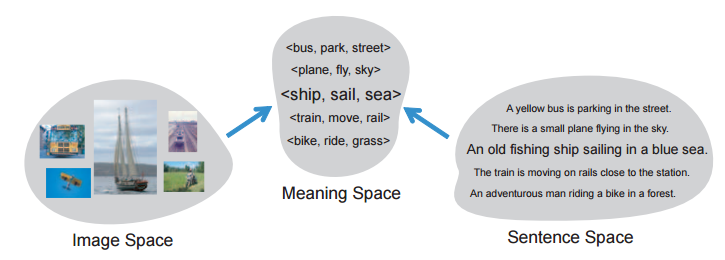
\includegraphics[scale=0.7]{./Imgs/farhadi2010every_fig1.png}
\caption[نگاشت تصویر به فضای معنایی]{
نگاشت تصویر به فضای معنایی. فضای معنایی شامل اطلاعات مطلوب برای استخراج در فرایند درک صحنه است. به ازای هر تصویر، یک سه‌تایی ایجاد می‌شود
\cite{Farhadi2010every}.
}
\label{fig:F2010EF1}
\end{figure}

مدل میدان تصادفی مارکف مورد استفاده در این پژوهش، یک مدل کوچک و ساده، شامل ۳ گره است. شکل \ref{fig:F2010EF2}
طرح‌واره‌ای از مدل میدان تصادفی مارکف مورد استفاده در این پژوهش را نمایش می‌دهد. همان‌طور که در شکل مشخص است،  به ازای هر کدام از میدان‌های تعریف شده در فضای معنایی، یک گره در این مدل وجود دارد. مقادیر مختلف در هر گره، برابر است با مقادیر مختلف موجود در میدان متناظر، در فضای معنا که با توجه به داده‌های مجموعه‌‌ ‌آموزشی مشخص می‌شوند. همین‌طور به ازای هر دو گره موجود در این مدل، یک یال بیان‌کننده ارتباط بین دو میدان در فضای معنایی وجود دارد.

برای استنتاج در این مدل، لازم است ابتدا فاکتور‌های مورد استفاده در مدل را شناخته و مقادیر آن‌ها را مشخص نماییم. در مدل پیشنهادی، دو نوع فاکتور تعریف شده است:

\begin{enumerate}
\item فاکتورهای گره\\
این فاکتورها، برای مشخص کردن میزان شباهت مقادیر مختلف گره با تصویر ورودی، تعریف شده‌‌اند. ویژگی‌‌های مورد استفاده برای مقداردهی این فاکتورها، شامل موارد زیر هستند:
\begin{enumerate}
	\item	 استفاده از آشکارکننده‌های\enfootnote{Detector}
	فلزنسوالب\enfootnote{Felzenszwaalb}، 
	به منظور محاسبه امتیاز اطمینان\enfootnote{Confidence Score} برای هر دسته از اجسام موجود در مجموعه‌داده\cite{felzenszwalb2008discriminatively}.\\
	پس از محاسبه امتیاز اطمینان همه دسته‌های موجود، دسته‌ای که بیشترین امتیاز را دارد می‌تواند به عنوان دسته‌ منتخب در میدان متناظر گره، انتخاب شود. در فرایند مقداردهی این ویژگی، قبل از انجام محاسبات، اطمینان حاصل می‌شود که از هر دسته موجود، حداقل یک تصویر در مجموعه‌داده وجود داشته باشد.
	\item استفاده از پاسخ دسته‌بندی‌کننده دیوالا\enfootnote{divvala}، ارائه شده در مقاله\cite{divvala2009empirical}
	\item استفاده از دسته‌بندی‌کننده مبتنی بر گیست\enfootnote{Gist-based classification response}
\end{enumerate}

\begin{figure}[h]
\center
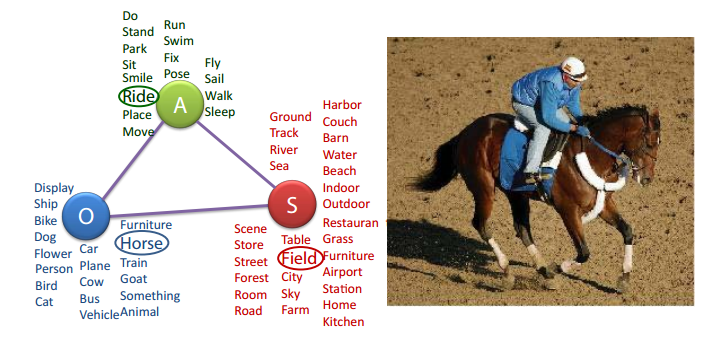
\includegraphics[scale=0.7]{./Imgs/farhadi2010every_fig2.png}
\caption[مدل میدان تصادفی مارکف در درک صحنه]{
طرح‌واره مدل میدان تصادفی مارکف ارائه شده در پژوهش \cite{Farhadi2010every} که شامل ۳ گره است. در این مدل، به ازای هر میدان از فضای معنا، یک گره وجود دارد و بین هر سه گره‌، به طور دو به دو، یک یال موجود است\cite{Farhadi2010every}.
}
\label{fig:F2010EF2}
\end{figure}

بر اساس مقادیر محاسبه شده برای ویژگی‌های بالا و با استفاده از الگوریتم ماشین بردار پشتیبان\enfootnote{Support Vector Machine (SVM)}، یک دسته‌بندی برای هر گره ارائه می‌شود که بیان‌کننده دسته‌ویژگی‌های مربوط به مقادیر مختلف گره است. با استفاده از این دسته‌بندی، با ورود هر تصویر، می‌توان برای هر مقدار در هر گره، یک امتیاز شباهت محاسبه نمود. استفاده از الگوریتم یافتن نزدیک‌ترین همسایه‌های موجود برای هر تصویر ورودی، بر اساس امتیاز شباهت محاسبه‌شده و میانگین‌گیری روی همسایه‌های استخراج شده، معیار خوبی از تخمین مقدار هر گره، به ازای هر تصویر ورودی ایجاد می‌کند. به این ترتیب، با ورود هر تصویر می‌توان برای هر کدام از گره‌های موجود در مدل، یک مقدار محتمل مشخص نمود. سه‌تایی شامل مقادیر محتمل بدست‌آمده در هر گره، سه‌تایی متناظر تصویر ورودی در فضای معنا را مشخص می‌کند.
\item فاکتورِ یال\\
این فاکتور، برای مشخص کردن میزان ارتباط مقادیر مختلف دو گره با یکدیگر در تصویر ورودی مورد استفاده قرار می‌گیرند.
\end{enumerate}

%%%%%%%%%%%%%%%%%%%%%%%%%%%%%%%%%%%%%%%%%
\subsubsection[استفاده از مدل میدان تصادفی شرطی]{استفاده از مدل میدان تصادفی شرطی\enfootnote{Conditional Random Field (CRF)}}
در این پژوهش، مساله درک صحنه در قالب یک مساله استنتاج با استفاده از مدل میدان تصادفی شرطی بیان شده است. مدل میدان تصادفی شرطی، یکی از پرکاربردترین مدل‌های گرافی احتمالی در زمینه درک صحنه است که پژوهش‌های متعددی از آن به عنوان مدل اصلی در درک صحنه استفاده کرده‌اند. به عنوان نمونه، در مقاله‌های 
\cite{Lin_2013_ICCV}
و
\cite{ladicky2010and}
از مدل میدان تصادفی شرطی به منظور توصیف صحنه استفاده شده است.\\

 پژوهش \cite{Lin_2013_ICCV} سعی در توصیف اجسام سه‌بعدی با استفاده از قطعه‌بندی تصاویر دوبعدی، هندسه سه‌بعدی و روابط بین صحنه و اجسام موجود، دارد. در این پژوهش، پس از استخراج ویژگی‌ها و اطلاعات بدست‌آمده از منابع مختلف، عمل استنتاج توسط یک مدل تصادفی شرطی انجام می‌شود که منجر به نگاشت تصویر ورودی به فضای معنایی می‌شود. همین‌طور در پژوهش \cite{ladicky2010and}، یک چارچوب کاری\enfootnote{Framework} احتمالی برای استنتاج درباره نواحی مختلف تصویر، اجسام موجود و ویژگی‌های مختلف آن‌ها مانند دسته‌بندی، موقعیت مکانی و ابعاد، مبتنی بر مدل میدان تصادفی شرطی، ارائه شده است. با توجه به وسعت و تعدد فعالیت‌های انجام شده، در این بخش، مرحله درک صحنه یک پژوهش انجام شده در زمینه تولید خودکار شرح بر تصاویر را مورد بررسی قرار می‌دهیم. لازم به ذکر است، مرحله تولید جملات توصیف‌کننده پژوهش مورد بحث، در فصل تولید جملات زبان طبیعی مورد بررسی قرار خواهد گرفت.
\\
در پژوهش\cite{fidler2013sentence}
از مدل میدان تصادفی شرطی برای توصیف صحنه و اجسام موجود در آن استفاده شده است. میدان‌های تصادفی در این مدل، شامل متغیرهای زیر هستند:
\begin{enumerate}
\item  متغیرهای تصادفی بیان‌کننده برچسب دسته متناظر قطعات مختلف هر تصویر به شیوه سلسله مراتبی دارای دو سطح
\item متغیرهای تصادفی باینری بیان‌کننده صحت دسته‌ تشخیص داده‌شده برای هر جسم
\end{enumerate}

شکل
\ref{fig:F2013SF1}
 طرح‌واره مدل سلسله‌مراتبی ارائه شده در پژوهش \cite{fidler2013sentence} را نمایش می‌دهد. همان‌طور که مشاهده می‌شود این مدل از دو سطح انتزاع، یکی برای برچسب قطعات مختلف تصویر و دیگری برای حضور یا عدم حضور هر دسته از اجسام در تصویر، تشکیل شده است.

\begin{figure}[h]
\center
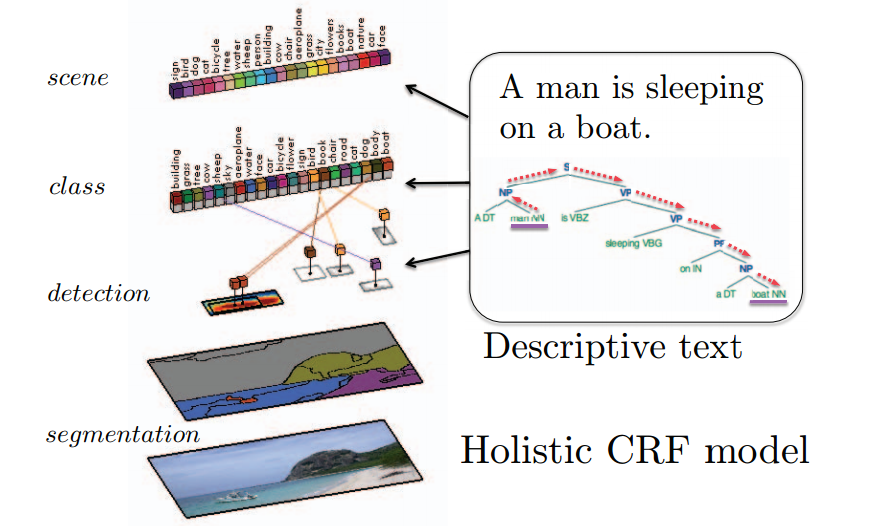
\includegraphics[scale=0.5]{./Imgs/fidler2013sentence_f1.png}
\caption[مدل سلسله‌مراتبی میدان تصادفی شرطی در درک صحنه]{طرح‌واره مدل سلسله مراتبی مبتنی بر میدان تصادفی شرطی که بر اساس اطلاعات بصری و اطلاعات جملات توصیف‌کننده شرح محتمل تصویر را تولید می‌نماید\cite{fidler2013sentence}.}
\label{fig:F2013SF1}
\end{figure}

دو دسته متغیر تصادفی مختلف، که هر یک نماینده متغیرهای تصادفی موجود در یکی از این سطوح انتزاع هستند، تعریف شده‌اند؛ 
متغیرهای تصادفی $X_i \in {1, \cdots,C}$ بیان‌کننده دسته قطعه $i$ام از سطح پایین سلسله مراتب و متغیرهای تصادفی $Y_j \in {1, \cdots,C}$ بیان‌کننده دسته قطعه $j$ام از سطح بالای سلسله مراتب.
به علاوه، دو دسته متغیر تصادفی دیگر به نام‌های $b_l$ و $z_k$ به ترتیب برای نمایش حضور یا عدم حضور یک تشخیص کاندید\enfootnote{Candidate Detection} و حضور یا عدم حضور جسم با دسته $k$ در تصویر، تعریف شده‌اند. با توجه به متغیرهای تعریف شده، مدل کلی میدان تصادفی شرطی را می‌توان معادل رابطه\ref{eq:crffidler} تعریف کرد. در این رابطه $\Psi_\alpha^{type}(a_\alpha)$ نماینده تابع پتانسیل تعریف شده روی متغیرهای مختلف است. با این تعریف، یافتن تخمین \lr{MAP}\enfootnote{MAP Estimation}، منجر به یافتن پاسخ مورد نظر می‌شود.
در ادامه، توابع پتانسیل مختلف که در این پژوهش تعریف شده‌اند، ارائه خواهد شد. لازم به ذکر است در تمام این موارد، برای سهولت، توابع پتانسیل به شکل لگاریتمی تعریف شده‌اند.
\begin{equation}
P(X,Y,b,z) = \frac{1}{Z} \mathlarger{\mathlarger{\Pi}}_{type} \mathlarger{\mathlarger{\Pi}}_\alpha \Psi_\alpha^{type}(a_\alpha)
\label{eq:crffidler}
\end{equation}

توابع پتانسیل مختلف تعریف شده در این پژوهش عبارتند از:

\begin{enumerate}
\item پتانسیل قطعه‌بندی یگانی\enfootnote{Unary Segmentation Potential}\\
پتانسیل قطعه‌بندی یگانی در هر قطعه و هر ابرقطعه\enfootnote{Supersegment} از تصویر، با استفاده از میانگین‌گیری روی امتیاز افزایش تکستون\enfootnote{Texton Boost} که در پژوهش \cite{ladicky2010graph} ارائه شده است، انجام می‌شود.
\item انطباق بین متغیرهای دو سطح انتزاع با یک‌دیگر\\
یک مقدار جریمه به ازای دسته‌های مخالف بین دو سطح در نظر گرفته‌ می‌شود تا در حد امکان، دسته‌های منتخب از بین سطوح مختلف، با یک‌دیگر انطباق داشته باشند. پتانسیل تعریف شده در این بخش معادل رابطه\ref{eq:phiijf} 
تعریف می‌شود.
	\begin{equation}
		\phi_{ij}(X_i, Y_j)=
			\left\{
				\begin{array}{ll}
					- \gamma		&	X_i \neq Y_j \\
					0			&	X_i	=	Y_j
				\end{array}							
			\right.
		\label{eq:phiijf}
	\end{equation}
در رابطه\ref{eq:phiijf}، پارامتر $\gamma$ در فرآیند یادگیری که منجر به بهینه‌سازی پارامترهای مختلف مدل می‌شود، به‌دست می‌آید.
\item پتانسیل انطباق تصویر و دسته جسم\\
برای اندازه‌گیری میزان انطباق هر کدام از دسته‌های موجود برای اجسام با تصویر ورودی، از معیار انطباق ارائه شده در پژوهش\cite{felzenszwalb2010object}
 توسط فلزنسوالب که به روش دی پی ام\enfootnote{DPM} مشهور است، استفاده شده است. برای کاهش تعداد پارامترها و افزایش کارایی مدل استفاده شده، برای هر تصویر حداکثر ۳ دسته جسم، به عنوان دسته‌های منتخب کاندید، در نظر گرفته می‌شوند.
\end{enumerate}


%%%%%%%%%%%%%%%%%%%%%%%%%%%%%%%%%%%%%%%%%
\subsubsection{استفاده از سایر مدل‌های گرافی احتمالی}
در بین پژوهش‌های موجود در زمینه درک صحنه با استفاده از روش‌های احتمالاتی، علاوه بر مدل‌های استاندارد، از مدل‌های مولد دیگر در پژوهش‌های متعددی استفاده شده است. در ادامه این بخش، به بررسی چند‌ نمونه از این مدل‌ها خواهیم پرداخت.

\begin{enumerate}
\item دسته‌بندی تصاویر بر اساس صحنه و اجسام موجود به طور توام\cite{li2007and}

مدل استفاده شده در این پژوهش، از تصاویر در سطح صحنه و سطح اجسام استفاده کرده و با یکپارچه‌سازی و تجمیع اطلاعات موجود در این دو سطح، اقدام به دسته‌بندی تصویر می‌نماید. شکل\ref{fig:l2007af1} 
مدل استفاده شده در این پژوهش را به منظور یکپارچه‌سازی و تجمیع اطلاعات حاصل از تحلیل صحنه و تشخیص اجسام موجود در آن، ارائه می‌دهد.


\begin{figure}[H]
\center
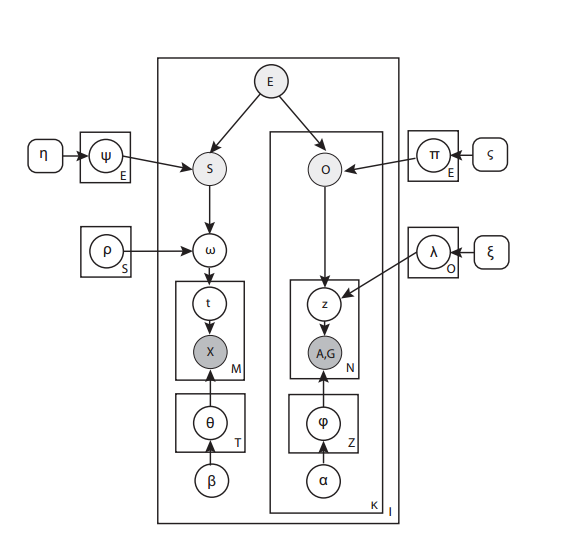
\includegraphics[scale=0.5]{./Imgs/li2007and_model.png}
\caption[مدل گرافی احتمالی مورد استفاده در پژوهش\cite{li2007and}]{مدل استفاده شده به منظور تجمیع اطلاعات صحنه و اجسام موجود در آن به منظور دسته‌بندی تصاویر\cite{li2007and}}
\label{fig:l2007af1}
\end{figure}

یکی از اهدافی که در این پژوهش دنبال می‌شود، برچسب‌گذاری معنایی\enfootnote{Semantic Labelling} تمام پیکسل‌های موجود در تصویر است. به همین منظور، تمام تصاویر مورد استفاده، به نواحی $10 * 10$ تقسیم شده و مورد استفاده قرار می‌گیرند. برای بررسی بهتر مدل، ابتدا متغیرهای تصادفی مورد استفاده را تعریف کرده و سپس به بررسی روند یادگیری و استنتاج مدل می‌پردازیم.
\\
متغیر تصادفی $X$ که حاوی اطلاعاتی مبتنی بر حضور یا عدم حضور دسته‌های مختلف صحنه است، در بخش تشخیص صحنه به‌کار می‌رود. اطلاعات این متغیر با استفاده از توصیف‌کننده سیفت\enfootnote{SIFT Descriptor} و به ازای هر ناحیه از تصویر، به‌دست می‌آید. برای بخش تشخیص اجسام موجود در صحنه، از دو منبع اطلاعاتی مختلف استفاده می‌شود. اطلاعات مربوط به حضور یا عدم حضور دسته‌های مختلف اجسام در متغیر تصادفی $A$ و اطلاعات مربوط به شکل کلی آن‌ها در متغیر تصادفی $G$ نمایش داده‌ می‌شود.
\\
هر گره از مدل ارائه شده، نماینده یک متغیر تصادفی است. گره‌هایی که با رنگ تیره مشخص شده‌اند، نماینده متغیرهایی هستند که در فرایند آموزش دیده می‌شوند و بقیه متغیرها، متغیرهای مخفی\enfootnote{Latent} هستند. گره‌های خاکستری روشن‌تر، متغیرهایی هستند که فقط در فرایند آموزش دیده‌ می‌شوند در حالی‌که متغیرهای تیره‌تر در هر دو فرایند آموزش و آزمون مشاهده می‌شوند.
\\
متغیر تصادفی $E$، نماینده یک دسته‌ از رخداد
\enfootnote{Event}
های ممکن است. توزیع احتمال اولیه این متغیر  تصادفی، یک توزیع یکنواخت فرض شده است که به هر تصویر ورودی، بر اساس همین توزیع، یک مقدار خاص از این متغیر تصادفی اختصاص داده می‌شود. با دانستن دسته رخداد موجود در تصویر، یک تصویر صحنه\enfootnote{Scene Image} متناظر با تصویر ورودی تولید می‌شود. با فرض وجود $S$ دسته صحنه مختلف در مجموعه‌داده، به هر تصویر، تنها یک دسته صحنه اختصاص داده می‌شود. روند اختصاص دسته صحنه به تصویر مطابق زیر است:
\begin{itemize}
\item[*]
ابتدا یک دسته اولیه مطابق با توزیع احتمال شرطی 
$P(S|E, \psi)$
به تصویر اختصاص داده می‌شود. $\psi$ یک پارامتر چندجمله‌ای
\enfootnote{Multinomial}
 حاکم بر توزیع احتمالاتی $S$ به شرط داشتن $E$ است. به علاوه، $\psi$ یک ماتریس به ابعاد $E * S$ و پارامتر $\eta$ یک بردار $S$ بعدی در نقش مقدار اولیه دیریکله
\enfootnote{Dirichlet prior}
 برای پارمتر $\psi$ است.
\item[*]
در قدم بعدی با داشتن مقدار $S$، پارامترهای $\omega$ را بر اساس احتمال 
$P(\omega|S, \rho)$
تولید می‌کنیم. از آن‌جا که $\omega$ پارامتر چندجمله‌ای گره‌های مخفی $t$ هستند، باید مجموع همه آن‌ها برابر با یک باشد. به علاوه، $\rho$ یک ماتریس به ابعاد $S * T$ و مقدار اولیه دیریکله برای پارامتر $\omega$ است که در آن $T$ تعداد کل $t$ها است.
\item[*] 
برای تولید هر یک از $M$ ناحیه تصویر (مقادیر متغیر تصادفی $X$) به شکل زیر عملی می‌کنیم:
\begin{itemize}
\item[-]
یک مقدار $t$ از توزیع احتمال $Mult(\omega)$ تولید می‌شود که مشخص‌کننده موضوعی\enfootnote{Topic} است که این ناحیه از تصویر مطابق با آن تولید شده است.
\item[-]
متغیر تصادفی $X$ از توزیع احتمالی 
$P(X|t,\theta)$ تولید می‌شود.
$\theta$ یک ماتریس به ابعاد
$T * V_s$ است که در آن
$V_s$ تعداد کلمات موجود در پایگاه داده مربوط به صحنه $s$  است.
به علاوه، $\theta$ یک پارامتر چندجمله‌ای برای $X$ است و $\beta$ مقدار اولیه دیریکله برای $\theta$.
\end{itemize}
\end{itemize}

همانند فرایندی که طی آن، تصویر صحنه به تصویر ورودی اختصاص داده می‌شود، فرایندی وجود دارد که طی آن تصویر اجسام\enfootnote{Object Image} به تصویر ورودی اختصاص داده می‌شود. بر خلاف صحنه، هر تصویر می‌تواند بیش از یک جسم داشته باشد. تعداد کل اجسام موجود در یک تصویر را با $K$ و تعداد کل دسته‌های موجود برای اجسام در مجموعه‌داده را با $O$ نمایش می‌دهیم. فرایند زیر برای هر یک از $K$ جسم موجود در تصویر اجرا می‌شود:

\begin{itemize}
\item[*]
ابتدا یک دسته جسم با توزیع احتمالی  
$P(O|E, \pi)$
به تصویر اختصاص داده می‌شود که در آن، $\pi$ یک ماتریس به ابعاد $E * O$ و $\zeta$ یک بردار به طول $O$ و مقدار اولیه دیریکله پارامتر $\pi$ است.
\item[*]
سپس با داشتن $O$ می‌توان تمام نواحی $A$ و $G$ مرتبط با دسته جسم را تولید نمود. فرایند تولید این نواحی به شکل زیر است:
	\begin{itemize}
	\item[-]
	متغیر تصادفی مخفی $z$ که مشخص کننده موضوع است، از توزیع احتمالی $Mutl(\lambda,|O)$ تولید می‌شود. متغیر $\lambda$ یک ماتریس به ابعاد $O * Z$ است که در آن  $Z$ تعداد کل مقادیر مختلف متغیر $z$ است. به علاوه $\xi$ مقدار اولیه دیریکله برای پارامتر $\lambda$ است.
	\item[-]
	نواحی مطلوب از توزیع احتمال $P(A,G|t, \phi)$ تولید می‌شوند که در آن، $\phi$ یک ماتریس به ابعاد $Z * V_o$ است. $V_o$ تعداد کل کلمات موجود در مجموعه‌داده، به ازای نواحی $A$ و $G$ است. پارامتر $\alpha$ مقدار اولیه دیریکله برای پارامتر $\phi$
است. 	
	\end{itemize}
\end{itemize}

با توجه به متغیرهای تصادفی توضیح داده شده در بالا، توزیع احتمالی توام کل سیستم را می‌توان مطابق با رابطه 
\ref{eq:liJP}
تعریف کرد.

\begin{equation}
\label{eq:liJP}\begin{split}
P(E,S,O,X,A,G,t,z,\omega |\rho ,\phi ,\lambda ,\psi ,\pi \theta) &= P(E)\cdot P(S|E,\psi)\cdot P(\omega|S,\rho) \\ 
&\cdot \mathlarger{\mathlarger{\Pi}}_{m=1}^M P(X_m|t_m,\theta)\cdot P(t_m|\omega) \\
&\cdot \mathlarger{\mathlarger{\Pi}}_{k=1}^K P(O_k|E,\pi)\\
&\cdot \mathlarger{\mathlarger{\Pi}}_{n=1}^N P(A_n,G_n|z_n,\phi)\cdot P(z_n|\lambda,O_k)
\end{split}
\end{equation}

به علاوه، با توجه به توضیحات ارائه شده در بالا، هر کدام از عبارات موجود در رابطه \ref{eq:liJP} را می‌توان با عبارات معادل آن‌ها که در روابط
\ref{eq:liSF}
تا
\ref{eq:liSL}
آمده، جایگزین نمود.

\begin{align}
&P(S|E,\psi) = Mult(S|E,\psi)
\label{eq:liSF}
\\
&P(\omega|S,\rho) = Dir(\omega|\rho_{j.}), S = j
\\
&P(t_m|\omega) = Mult(t_m|\omega)
\\
&P(X_m|t_m,\theta) = P(X_m|\theta_{j.}), t_m = j
\\
&P(O_k|E,\pi) = Mult(O_k|E,\pi)
\\
&P(z_n|\lambda,O_k) = Mult(z_n|\lambda,O_k)
\\
&P(A_n,G_n|z_n,\phi) = P(A_n,G_n|\phi_{j.}), z_n = j
\label{eq:liSL}
\end{align}

درک صحنه در این پژوهش، محدود به استخراج سه دسته اطلاعات زیر از تصویر است:

\begin{enumerate}
\item رخدادی که در تصویر به نمایش گذاشته شده است.
\item صحنه‌ای که تصویر در آن ایجاد شده است.
\item اجسامی که در تصویر حضور دارند.
\end{enumerate}

با توجه به این محدودیت و با در نظر گرفتن مدل ارائه شده، استفاده از تخمین بیشینه احتمال\enfootnote{Maximum Likelihood}، می‌تواند برای استخراج اطلاعات مطلوب مفید باشد. از همین رو، تخمین بیشینه احتمال، در سه سطح مختلف (هر سطح برای یک دسته از اطلاعات مطلوب) اعمال می‌شود. در سطح اجسام، احتمال رخداد تصویر ورودی به شرط اجسام موجود مطابق با رابطه 
\ref{eq:liPIO}، احتمال رخداد تصویر ورودی به شرط صحنه، مطابق با رابطه 
\ref{eq:liPIS}
و احتمال رخداد تصویر ورودی به شرط دسته رخداد به نمایش‌گذاشته شده در تصویر، مطابق با رابطه 
\ref{eq:liPIE}
محاسبه می‌شوند.
\begin{align}
&P(I|O) = \ML{\Pi}_{n=1}^N \ML{\Sigma}_j P(A_n,G_n|z_j,O) P(z_j|O)
\label{eq:liPIO}
\\
&P(I|S,\rho,\theta) = \int P(\omega|\rho,S)(\ML{\Pi}_{m=1}^M \ML{\Sigma}_{t_m} P(t_m|\omega) P(X_m|t_m, \theta) ) d\omega
\label{eq:liPIS}
\\
&P(I|E) \propto \ML{\Sigma}_j P(I|O_j) P(O_j|E) P(I|S) P(S|E)
\label{eq:liPIE}
\end{align}

فرایند یادگیری این مدل، شامل یافتن بهترین مقادیر برای پارامترهای 
$\{\psi,\rho,\pi,\lambda,\theta,\beta\}$
است.
این فرایند برای سه پارامتر 
$\{\psi,\rho,\theta\}$ 
با استفاده از روش انتقال پیام متغیر\enfootnote{Variational Message Passing} و برای سه پارامتر
$\{\pi,\lambda,\beta\}$
با استفاده از نمونه‌برداری گیبس\enfootnote{Gibbs Sampling} انجام می‌شود.
\\
آزمایشات انجام شده در این پژوهش، بر روی یک مجموعه‌داده شامل تصاویر از ۸ دسته ورزشی مختلف که در هر دسته، بین 137 تا 250 تصویر مختلف وجود دارد، انجام شده‌اند. از جمله چالش‌های موجود در این مجموعه‌داده می‌توان به وجود زمینه‌های متنوع و پیچیده در تصاویر، تنوع دسته‌های مختلف اجسام موجود، تنوع اندازه اجسام موجود از یک دسته، تنوع حالت اجسام، تنوع تعداد نمونه‌های یک جسم در یک تصویر و کوچک بودن بیش از اندازه ابعاد اجسام در تصویر اشاره کرد. شکل
\ref{fig:lid}
نمونه‌ای از تصاویر موجود در این مجموعه‌داده را نمایش می‌دهد.

\begin{figure}[H]
\center
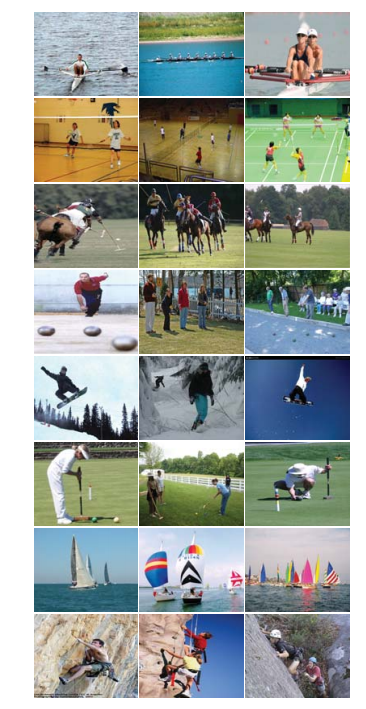
\includegraphics[scale=0.7]{./Imgs/li2007and_dataset.png}
\caption{نمونه تصاویر موجود در مجموعه‌داده مورد استفاده \cite{li2007and}}
\label{fig:lid}
\end{figure}

استفاده از مدل کامل ارائه شده در این پژوهش، منجر به تشخیص صحیح 73.4\% از تصاویر شده است. شکل
\ref{fig:liCM}
 ماتریس درهم‌ریختگی
\enfootnote{Confusion Matrix}
 مربوط به این مدل را نمایش می‌دهد. همان‌طور که در این ماتریس مشخص است، کمترین نرخ تشخیص در بین دسته‌های ورزشی موجود در این مدل، 52\% و بیشترین نرخ تشخیص 92\% است.

\begin{figure}[H]
\center
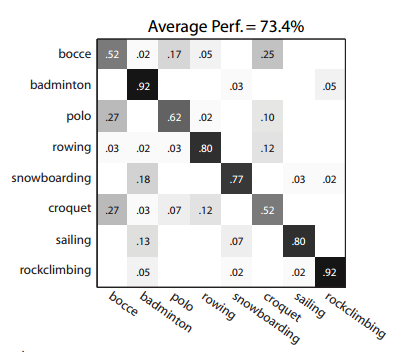
\includegraphics[scale=0.8]{./Imgs/li2007and_confmat.png}
\caption[ماتریس درهم‌ریختگی مدل کامل ارائه شده در \cite{li2007and}]{ماتریس درهم‌ریختگی مدل کامل ارائه شده برای مجموعه‌داده شامل ۸ دسته تصویر ورزشی. \cite{li2007and}}
\label{fig:liCM}
\end{figure}

بسته به میزان استفاده از اطلاعات مختلف استخراج شده برای استنتاج، مدل‌های مختلفی به‌وجود می‌آیند که در شکل
\ref{fig:liCMP}
نتایج عملکرد هریک از این مدل‌ها با مدل‌های دیگر مقایسه شده است.
همان‌طور که در شکل \ref{fig:liCMP}
مشخص است، بهترین کارایی مربوط به مدل کامل است. در صورتی‌که در مدل، فقط از اطلاعات مربوط به صحنه استفاده شود، نتایج بدست‌آمده اگرچه با نتایج مدل کامل قابل مقایسه نیست، از نتایج مدل مبتنی بر اطلاعات جسم بهتر است.

\begin{figure}[H]
\center
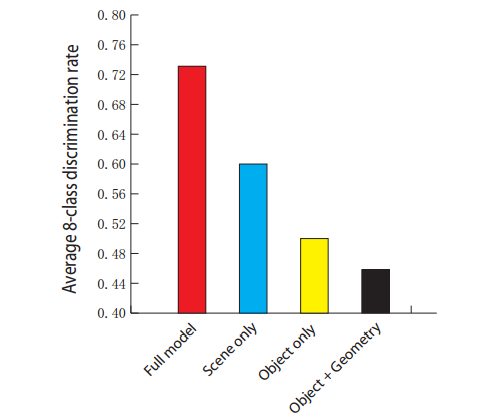
\includegraphics[scale=0.4]{./Imgs/li2007and_compar.png}
\caption[نتیجه مقایسه مدل‌های مختلف در \cite{li2007and}]{نتیجه مقایسه مدل‌های مختلف به‌وجود آمده بسته به سطح اطلاعات مورد استفاده برای استنتاج. \cite{li2007and}}
\label{fig:liCMP}
\end{figure}

شکل
\ref{fig:liR}
نتایج نهایی به‌دست آمده از مدل را نمایش می‌دهد. در این شکل، تصاویر موجود در هر سطر نماینده تصاویر موجود در یکی از دسته‌های ورزشی هستند. ستون اول برچسب به‌دست آمده از رخداد موجود در تصویر، ستون دوم برچسب‌های تشخیص داده شده مربوط به اجسام موجود، ستون سوم برچسب اختصاص داده‌شده مربوط به دسته صحنه و ستون چهارم توزیع مرتب شده اجسام به شرط رخداد را به نمایش می‌گذارند. در نمودارهای موجود در ستون چهارم، محور افقی شامل نام اجسام و محور عمودی مقدار توزیع را نمایش می‌دهد.

\begin{figure}[H]
\center
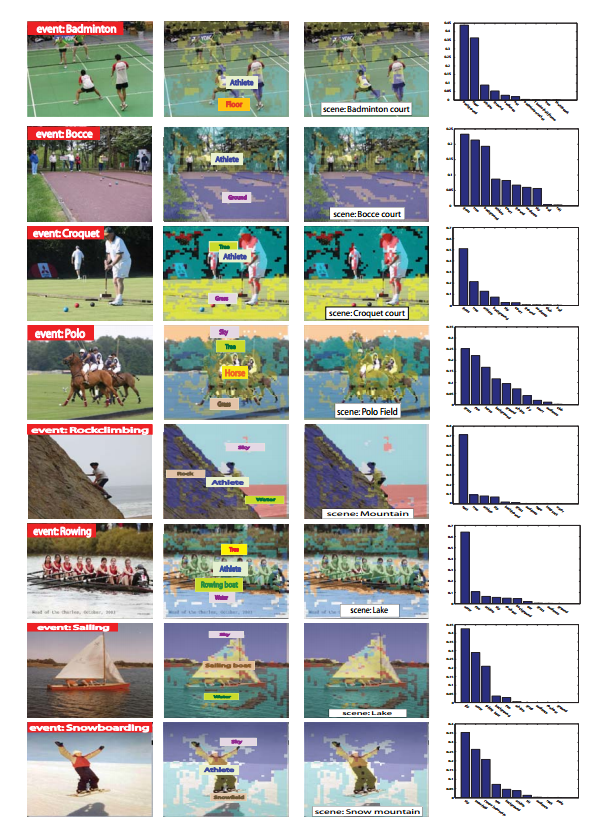
\includegraphics[height=0.8\textheight]{./Imgs/li2007and_res1.png}
\caption{نتایج نهایی به‌دست آمده از مدل بر روی تصاویر. \cite{li2007and}}
\label{fig:liR}
\end{figure}



%%%%%%%%%%%%%%%%%%%%%%%%%%%%%%%%%%%%%%%%%%%%%%%%%%%%
%\item حاشیه‌نویسی تصویر\enfootnote{Image Annotation} با استفاده از قطعه‌بندی و دسته‌بندی صحنه و اجسام موجود\cite{li2009towards}
%
%
%
%
%
%\item درک صحنه بر اساس نواحی مختلف تصویر، اجسام موجود و روابط سه‌بعدی بین ‌آن‌ها\cite{gould2009decomposing}
\end{enumerate}

%%%%%%%%%%%%%%%%%%%%%%%%%%%%%%%%%%%%%%%%%
\subsection{روش‌های مبتنی بر شبکه‌های عصبی کانولوشنی عمیق}

علاوه بر فعالیت‌هایی که در زمینه تولید خودکار شرح بر تصاویر با رویکرد احتمالاتی انجام شده‌اند، تعداد زیادی از پژوهش‌گران تلاش می‌کنند تا با استفاده از روش‌‌های مبتنی بر شبکه‌های عصبی با این چالش روبرو شوند. در این بخش تعدادی از پژوهش‌هایی را که با استفاده از شبکه‌های عصبی سعی در درک صحنه‌های موجود در تصاویر دارند را مورد بررسی قرار می‌دهیم. شایان ذکر است، در این بخش تنها به بررسی بخشی از پژوهش‌ها که مربوط به درک صحنه است می‌پردازیم و بخش‌هایی از این پژوهش‌ها که مربوط به تولید جملات زبان طبیعی متناسب با تصویر و صحنه درک شده است را در فصل تولید جملات زبان طبیعی بررسی خواهیم نمود.
\\
یکی از مهم‌ترین عملیات‌هایی که به نحوی در تمام پژوهش‌های قبلی وجود داشت، اختصاص یک معنا به قطعه‌های مختلف یک تصویر است. این چالش، در پژوهش‌های مرتبط با تولید خودکار شرح بر تصاویر که با استفاده از روش‌های مبتنی بر شبکه‌های عصبی به دنبال حل مشکل هستند نیز مطرح است. در ابتدا به بررسی یکی از روش‌های اختصاص معنا به هر قطعه ازتصویر می‌پردازیم.

\subsubsection[اختصاص معنا به قطعه‌های مختلف تصویر]{اختصاص معنا به قطعه‌های مختلف تصویر\cite{Girshick_2014_CVPR}}
در پژوهش 
\cite{Girshick_2014_CVPR}
روشی ارائه شده است که با استفاده از یک شبکه عصبی کانولوشنی عمیق، علاوه بر این که می‌تواند یک تصویر را به شکل پایین به بالا، در قالب نواحی سلسله‌مراتبی قطعه‌بندی کند، قادر به استفاده به عنوان یک شبکه از پیش آموزش  دیده‌شده در پژوهش‌های مرتبط دیگر باشد.
\\
فرایند تشخیص اجسام در این پژوهش از سه بخش اصلی تشکیل شده است:
\begin{enumerate}
\item
طرح پیشنهاداتی برای نواحی به طور مستقل از دسته‌بندی\enfootnote{Category-independent region proposals}
\item 
یک شبکه عصبی عمیق کانولوشنی که وظیفه استخراج ویژگی برای هر ناحیه را بر عهده دارد (طول بردار ويژگی استخراج شده برای تمام نواحی یکسان است).
\item
مجموعه‌ای از ماشین‌های بردار پشتیبان خطی مخصوص هر دسته
\end{enumerate}
در ادامه به بررسی نحوه پیشنهاد نواحی و شبکه عصبی کانولوشنی عمیق مورد استفاده در ای پژوهش می‌پردازیم.

\begin{enumerate}
\item طرح پیشنهاد نواحی\\
روش‌های مختلفی برای پیشنهاد نواحی ارائه شده‌اند که در اینجا از روشی موسوم به جستجوی انتخابی\enfootnote{Selective Search} استفاده می‌شود. نسخه‌های مختلفی از این روش ارائه شده است. نسخه ارائه شده در پژوهش
\cite{uijlings2013selective}،
یکی از سریع‌ترین نسخه‌های ارائه شده است که در این بخش از همین روش استفاده می‌شود.
\\
در پژوهش 
\cite{uijlings2013selective}
دو ویژگی‌ مطرح شده است که یک جستجوی انتخابی برای ارائه نواحی معنایی تصویر باید آن‌ها را داشته باشد. ویژگی اول این است که اجسام موجود در فضا می‌توانند در هر اندازه‌ای باشند و در نتیجه نواحی ارائه شده باید بتوانند ابعاد مختلف داشته باشند. این ویژگی عموما با روش‌های سلسله‌مراتبی قابل دست‌یابی است. ویژگی دوم این است که نواحی مختلف باید براساس  ویژگی‌های مختلفی تولید شوند. در صورتی‌که یک ویژگی مثل رنگ، بافت، روشنایی یا مواردی از این دست، به عنوان تنها ویژگی برای تشخیص نواحی به کار گرفته شود، الگوریتم قادر به ارائه نواحی مناسب در شرایط مختلف نخواهد بود. بنابراین ترکیب چند معیار و ویژگی باید برای تشخیص نواحی مورد استفاده قرار بگیرد. 
\\
برای دست‌یابی به ویژگی اول، ابتدا نواحی اولیه کوچکی روی تصویر ایجاد می‌شود. سپس با اتخاذ یک روش حریصانه و تعریف یک معیار شباهت بین نواحی همسایه، ناحیه‌هایی که شباهت زیادی با یک‌دیگر دارند و همسایه هستند، با هم ترکیب شده و یک ناحیه بزرگ‌تر ساخته می‌شود. به این ترتیب یک روش سلسله‌مراتبی برای ساخت نواحی با ابعاد مختلف به‌دست ‌می‌آید.برای دست‌یابی به ویژگی دوم، از فضاهای رنگی مختلف، معیارهای شباهت مختلف و نواحی اولیه متفاوت و ترکیب پاسخ این ویژگی‌ها با هم برای ارائه نواحی و ترکیب نواحی کوچک‌تر استفاده می‌شود.

\item شبکه عصبی کانولوشنی عمیق (استخراج ویژگی‌ها)\\
در این بخش از یک شبکه عصبی کانولوشنی عمیق از پیش‌آموزش‌دیده‌ برای استخراج ویژگی ‌از هر ناحیه ارائه شده در قسمت قبل، استفاده می‌شود. بردار ویژگی استخراج شده برای هر ناحیه یک بردار شامل 4096 مولفه است که خروجی شبکه کریشفسکی\enfootnote{Krizhevsky}
آزمایش شده در چالش دسته‌بندی اجسام مسابقه  \lr{ImageNet} است. اطلاعات دقیق درباره این شبکه عصبی در پژوهش 
\cite{krizhevsky2012imagenet}
در دسترس است.

\end{enumerate}

شبکه عصبی کانولوشنی عمیق ارائه شده در این پژوهش با استفاده از یک مجموعه‌داده\enfootnote{ILSVRC 2012} آموزش دیده شده است. از این شبکه عصبی که تحت عنوان \lr{RCNN}\enfootnote{Regional Convolutional Neural Network} شناخته می‌شود می‌توان به عنوان یک شبکه از پیش‌آموزش‌دیده استفاده کرد.

\subsubsection[ناحیه‌بندی عمیق تصاویر به منظور نگاشت دوطرفه جملات و تصاویر]{ناحیه‌بندی عمیق تصاویر به منظور نگاشت دوطرفه جملات و تصاویر\cite{karpathy2014deep}}

مدل ارائه شده در این پژوهش، مدلی است که قادر به نگاشت دوطرفه تصاویر و جملات به یک‌دیگر است. شکل\ref{fig:k2014DM} طرح‌واره‌ای از این مدل را نمایش می‌دهد. ورودی مدل در سمت چپ، تصاویر و در سمت راست، جملات هستند. در این مدل، ابتدا تصاویر ورودی با استفاده از یک شبکه عصبی \lr{RCNN} تبدیل به نواحی مختلف شده و برای هر ناحیه یک بردار ویژگی 4096 بعدی استخراج می‌شود. سپس با اعمال روش خاصی روی جملات ورودی از سمت راست (که در بخش تولید جملات زبان طبیعی به بررسی آن خواهیم پرداخت) قطعات مختلف موجود در جملات نیز استخراج شده و بین هر قطعه از جمله با تمام نواحی استخراج شده از تصویر یک معیار شباهت محاسبه می‌شود و شبیه‌ترین قطعه جمله با ناحیه مربوط به خود در تصویر، جفت می‌شوند.

\begin{figure}[H]
\center
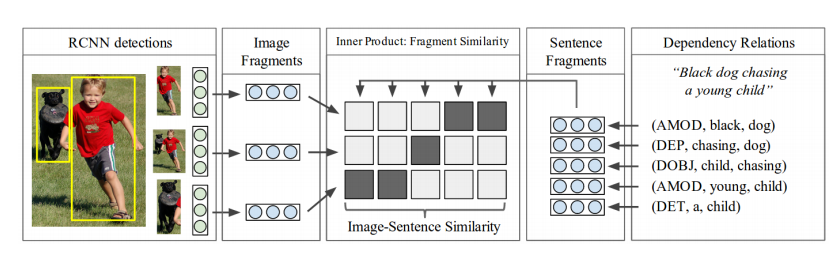
\includegraphics[scale=0.6]{./Imgs/karpathy2014deep_model.png}
\caption[طرح‌واره عملکرد روش \lr{RCNN}]{مدل استفاده شده برای نگاشت دو‌طرفه تصاویر و جملات به یک‌دیگر با استفاده از شکبه‌ عصبی عمیق کانولوشنی.\cite{karpathy2014deep}}
\label{fig:k2014DM}
\end{figure}

در این پژوهش پس از ناحیه‌بندی تصویر توسط شبکه \lr{RCNN}، برای هر تصویر ۱۹ ناحیه استخراج می‌شود. این ۱۹ ناحیه در کنار تصویر اصلی، یک مجموعه شامل ۲۰ تصویر ایجاد می‌کنند که در پردازش‌های بعدی مورد استفاده قرار خواهند گرفت. در این مرحله باید تمام تصاویر موجود را با استفاده از یک نگاشت به فضای برداری ویژگی‌ها تبدیل نمود. برای این کار از رابطه\ref{eq:k2014ISV}
استفاده می‌شود. در این رابطه، $I_b$ مجموعه تمام پیکسل‌های موجود در ناحیه $b$،
$RCNN_{\theta_c}$
شبکه عصبی آموزش‌دیده است که در آن $\theta_c$ مجموعه پارامترهای بهینه موجود در شبکه است. بردار حاصل $\nu_i$ برای تصویر $i$ام، بردار نگاشت تصویر به فضای معنایی خواهد بود که محاسبه مقادیر آن مبتنی بر پیشنهاد نواحی معنایی مختلف و محاسبه ويژگی‌های مختلف روی هر ناحیه است.

\begin{equation}
\nu = W_m[RCNN_{\theta_c}(I_b)] + b_m
\label{eq:k2014ISV}
\end{equation}

از طرفی با در نظر گرفتن بردار $s_j$ به عنوان بردار حاصل از نگاشت جمله $j$ام به فضای معنایی و در نظر گرفتن ضرب داخلی به عنوان شباهت، $\nu_i^T \cdot s_j$
معیار شباهت بین یک تصویر و یک جمله را تعریف می‌کند.
با توجه به توضیحات ارائه شده، می‌توان تابع هدف را برای شبکه کلی معادل سیستم ارائه داد. دو هدف اصلی در این شبکه قابل تعریف است:
\begin{enumerate}
\item رتبه‌بندی سراسری\\
 تصاویر و جملاتی که در فرایند محاسبات شبکه عصبی بیشترین شباهت را با یک‌دیگر دارند باید در واقعیت هم بیشترین شباهت و ارتباط را داشته باشند.
\item هم‌ترازسازی ناحیه‌ای\enfootnote{Fragment Alignment}\\
نواحی استخراج شده تصویر و عبارات استخراج شده جملات که در محاسبات شبکه عصبی بیشترین شباهت را با یک‌دیگر دارند، باید در واقعیت هم بیشترین شباهت و ارتباط را داشته باشند.
\end{enumerate}

با توجه به مطالب گفته شده، می‌توان تابع هدف کلی را مطابق با رابطه\ref{eq:k2014Obj}
تعریف کرد.
در این رابطه، $\Theta$ مجموعه پارامترهای شبکه عصبی شامل 
$\{W_m,b_m,\theta_c,W_e,W_R\}$
است (پارامترهای $W_e$ و‌ $W_R$ مربوط به بخش تحلیل جمله هستند که در فصل مربوطه بررسی خواهند شد). $C_F$ تابع هدف هم‌ترازسازی ناحیه‌ای، $C_G$ تابع هدف سراسری، $\alpha$ و $\beta$ دو ابرپارامتر\enfootnote{Hyperparameter} (با آزمون و خطا تعیین می‌شوند) و $||\Theta||_2^2$ یک عبارت تنظیم‌کننده\enfootnote{Regularization Term} هستند.

\begin{equation}
C(\Theta) = C_F(\Theta) + \beta C_G(\Theta) + \alpha ||\Theta||_2^2
\label{eq:k2014Obj}
\end{equation}

در ادامه به تعریف هریک از اهداف بیان‌شده می‌پردازیم.

\begin{enumerate}
\item هم‌ترازسازی ناحیه‌ای 

هدف از هم‌ترازسازی ناحیه‌ای این است که اگر عبارتی از یک جمله با یک تصویر شباهت زیادی پیدا کرد، حداقل یک ناحیه از تصویر وجود داشته باشد که نمایش‌دهنده این عبارت باشد و بقیه نواحی تصویر، ارتباط کمی با این عبارت داشته باشند. به عبارت بهتر، در صورتی‌که شباهت یک عبارت از یک جمله با یک تصویر از حدی بیشتر شد، شباهت حداقل یکی از نواحی موجود در تصویر با این عبارت زیاد شده و شباهت بقیه نواحی تصویر با آن کم شود. این فرض در سه حالت، رد می‌شود. اولین حالت، حالتی است که در آن ناحیه‌ای که در واقه نمایش‌دهنده عبارت است، توسط \lr{RCNN} تشخیص داده نشده باشد. دومین حالت، حالتی است که عبارت موجود به هیچ بخشی از ویژگی‌های بصری تصویر اشاره نکند و آخرین حالت، حالتی است که عبارت توصیف‌کننده، در هیچ یک از تصاویر دیگر تکرار نشده باشد در صورتی‌که ممکن است تصاویر دیگری هم وجود داشته باشند که شامل ویژگی‌های بصری متناظر با عبارت باشند. با توجه به شرایطی که فرض در آن‌ها نقض می‌شود، می‌توان آن را یک فرض خوب تلقی کرد که در اکثر موارد عملکرد خوبی دارد.
\\
رابطه\ref{eq:k2014C0}
تابع هدف هم‌ترازسازی ناحیه‌ای را تعریف‌ می‌کند. در این رابطه، $y_{ij}$ برای تصویر $i$ام و جمله $j$ام در صورتی‌که با هم در مجموعه‌داده حضور داشته باشند، +1 و در غیر این‌ صورت، -1 خواهد شد.

\begin{equation}
C_0(\Theta) = \ML{\Sigma}_i \ML{\Sigma}_j max(0 , 1 - y_{ij} \nu_i^T \cdot s_j)
\label{eq:k2014C0}
\end{equation}

تابع $C_0$ تعریف شده، باعث می‌شود در حالاتی که تصویر و عبارت، در مجموعه‌داده، با یک‌دیگر وارد شده باشند امتیاز تابع هدف بیشتر از +1 شود و در غیر این‌صورت از -۱ کمتر شود. شکل\ref{fig:k2014dCFG}،
 دو نمونه از تصاویر و جملات موجود در مجموعه‌داده را نمایش می‌دهد. 
 $C_0$ 
 در سلول‌هایی که با رنگ قرمز مشخص شده‌اند، امتیاز را به سمت کمتر از -1 حرکت می‌دهد و در بقیه سلول‌ها به سمت بیشتر از +1.

به عبارت بهتر، $C_0$ یک امتیاز برای مجموع تفاوت‌های نواحی مختلف از تصاویر با عبارات مختلف جملات است. به دلیل این‌که این معیار، باعث دیده نشدن موارد کم‌یاب می‌شود، با متغیر گرفتن پارامتر $y_{ij}$ سعی در یافتن کمترین مقدار آن می‌کنیم. رابطه 
\ref{eq:k2014CF}
معیار متناظر با هدف کلی هم‌ترازسازی ناحیه‌ای را بیان می‌کند.

\begin{align}
&C_F(\Theta) = min_{y_{ij}} C_0(\Theta)
\nonumber
\\
&s.t. \ML{\Sigma}_{i \in p_j} \frac{y_{ij} + 1}{2} \geq 1 \land
&y_{ij} = -1, \forall i,j ; m_\nu(i) \neq m_s(j) \land y_{ij} \in \{+1, -1\}
\label{eq:k2014CF}
\end{align}

در این رابطه، $p_j$ مجموعه تصاویر موجود در کیسه‌ مثبت\enfootnote{Positive Bag} مربوط به عبارت $j$ام است. شایان ذکر است، تنها تصاویری که در مجموعه‌داده همراه با عبارت $j$ام مشاهده شده‌اند در کیسه‌ مثبت مربوط به این عبارت قرار می‌گیرند و بقیه تصاویر در کیسه منفی\enfootnote{Negative Bag} این عبارت قرار می‌گیرند. $m_\nu(i)$ و $m_s(j)$ به ترتیب، شماره تصویر و عبارت را در مجموعه‌داده مشخص می‌کنند. 

\begin{figure}[H]
\center
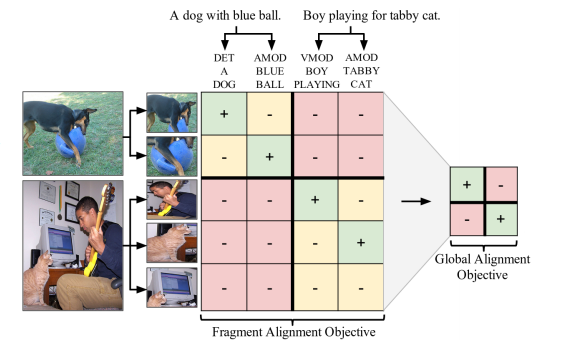
\includegraphics[scale=0.7]{./Imgs/karpathy20014deep_CFG.png}
\caption[نتایج عملکرد اهداف تعریف‌شده در روش \lr{RCNN} برای هم‌ترازسازی تصاویر و جملات]{دو نمونه از تصاویر و جملات مرتبط با آن‌ها و نتایج  عملکرد اهداف تعریف‌شده روی آن‌ها. سطرها نمایش‌دهنده نواحی مختلف تصویر و ستون‌ها نمایش ‌دهنده قطعه‌های مختلف جملات هستند. سلول‌های قرمز رنگ حالاتی هستند که در آن‌ها $y_{ij} = -1$، سلول‌های زرد نمایش‌دهنده اعضای کیسه‌های مثبت هستند که در آن‌ها $y_{ij} = -1$ است. \cite{karpathy2014deep}}
\label{fig:k2014dCFG}

\end{figure}

\item رتبه‌بندی سراسری

هدف از رتبه‌بندی سراسری این است که شباهت بین یک تصویر و یک جمله، بیشینه شود اگر و تنها اگر تصویر و جمله در واقعیت نیز بیشترین شباهت را به یک‌دیگر داشته باشند. برای این منظور، ابتدا یک امتیاز شباهت بین یک تصویر و یک جمله تعریف می‌شود. این امتیاز مطابق با رابطه\ref{eq:k2014CGS}
تعریف شده و برابر است با میانگین امتیاز شباهت دوبه‌دوی نواحی مختلف تصویر با عبارات مختلف جمله.

\begin{equation}
S_{kl} = \frac{1}{|g_k| (|g_l| + n)} \ML{\Sigma}_{i \in g_k}\ML{\Sigma}_{j\in g_l}max(0,\nu_i^T\cdot s_j)
\label{eq:k2014CGS}
\end{equation}

از آن‌جا که برای دسته‌بندی از روش \lr{mi\_SVM} استفاده می‌شود، تمام امتیازها به صفر محدود می‌شوند. مقدار $n$ که در مخرج کسر اضافه شده است، به صورت تجربی و با آزمون و خطا به‌دست آمده که نتایج را بهبود می‌بخشد. مقدار پیشنهاد شده در پژوهش، $n = 5$ است. تابع کلی هدف سراسری مطابق با رابطه \ref{eq:k2014CG}
تعریف می‌شود.

\begin{equation}
C_G(\Theta) = \ML{\Sigma}_k(
\ML{\Sigma}_l max(0, S_{kl} - S{kk} + \Delta) + 
\ML{\Sigma}_l max(0, S_{lk} - S{kk} + \Delta) 
)
\label{eq:k2014CG}
\end{equation}

در رابطه ارائه شده، $\Delta$ یک ابرپارامتر است که با آزمون و خطا به‌دست می‌آید. عبارت اول درون پرانتز بیان‌کننده امتیاز تصویر و عبارت دوم بیان‌کننده امتیاز جمله هستند.
\end{enumerate}


شکل\ref{fig:k2014res1}
نتایج روش پیشنهاد شده در این پژوهش را ارائه می‌دهد. همان‌طور که در شکل مشخص است، این شبکه قادر به تشخیص اجسام مختلف در تصویر و تولید یک سه‌تایی متناظر هر جسم (ناحیه معنایی) مبتنی بر جملات موجود در مجموعه‌داده مورد استفاده است.

\begin{figure}[H]
\center
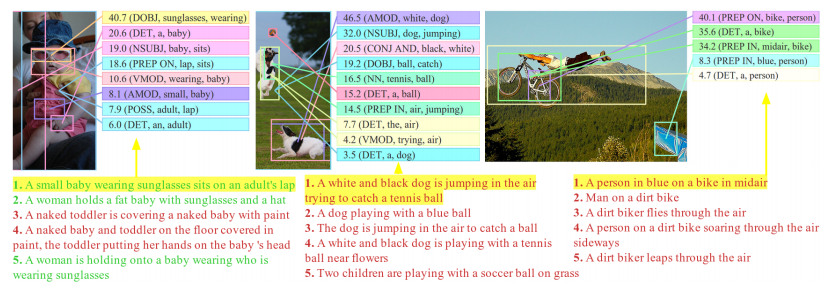
\includegraphics[scale=0.5]{./Imgs/karpathy2014deep_res1.png}
\caption[نتایج نهایی روش \lr{RCNN}]
{نتایج نهایی شبکه عصبی ارائه شده. برای هر ناحیه معنایی از تصویر، یک سه‌تایی مبتنی بر جملات موجود در مجموعه‌داده تولید شده است. همین‌طور 5 جمله تولید شده برای هر تصویر به ترتیب امتیاز، درج شده‌اند.\cite{karpathy2014deep}}
\label{fig:k2014res1}
\end{figure}

به علاوه، با توجه به مدل ارائه شده و نگاشت دوطرفه موجود بین تصاویر و جملات، می‌توان با ورودی دادن یک جمله، تصاویر مربوط به آن جمله را استخراج نمود. شکل\ref{fig:k2014res2}
با ثابت در نظر گرفتن جملات، تصاویر مربوط به هر جمله را استخراج و نمایش داده است. هر سطر از این شکل، نمایش‌دهنده تصاویر استخراج شده مرتبط با جمله موجود در آن سطر است.



\begin{figure}[H]
\center
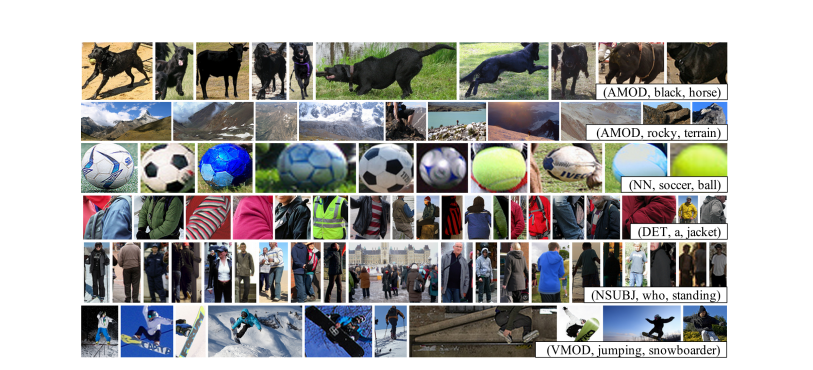
\includegraphics[scale=0.6]{./Imgs/karpathy2014deep_res2.png}
\caption[نتایج حاصل از جستجوی جملات در روش \lr{RCNN}]{نتایج حاصل از جستجوی جملات. با ورودی دادن یک جمله، شبکه عصبی ارائه شده در این پژوهش، قادر به استخراج تصاویر مربوط به آن جمله است.\cite{karpathy2014deep}}
\label{fig:k2014res2}
\end{figure}

روش ارائه شده در این پژوهش، به طور کامل و دقیق در پژوهش \cite{Karpathy_2015_CVPR} هم مورد استفاده قرار گرفته است، با این تفاوت که در فرایند تحلیل جمله، تغییراتی ایجاد شده است. جزئیات این روش در فصل تولید جملات زبان طبیعی مورد بررسی قرار خواهد گرفت.

%%%%%%%%%%%%%%%%%%%%%%%%%%%%%%%%%%%%5
\subsection{جمع‌بندی}

اولین مرحله از فرایند تولید خودکار شرح برای تصاویر، مرحله درک صحنه است. در این مرحله، تصاویر ورودی تحت عملیات مختلفی به فضای معنایی نگاشت می‌شوند. فضای معنایی در این‌جا، می‌تواند فضای شامل میدان‌های اطلاعاتی از پیش تعیین شده (مانند فضای سه‌تایی‌های «جسم، رخداد، صحنه») یا فضای بردار ویژگی‌ها باشد.
\\
روش‌های مختلفی برای نگاشت تصویر ورودی به فضای معنایی ارائه شده است که به طور کلی می‌توان عموم آن‌ها را به دو بخش تقسیم کرد:
\begin{enumerate}
\item
روش‌های مبتنی بر مدل‌های گرافی احتمالاتی\\
در این روش‌ها با استفاده از مدل‌های استاندارد گرافی احتمالاتی موجود یا با ارائه یک مدل گرافی احتمالاتی، تصویر ورودی به فضای معنایی نگاشت می‌شود. در روش‌های مبتنی بر این مدل‌ها، با ارائه یک توزیع احتمال برای نقاط مختلف در فضای معنایی، محتمل‌ترین نقطه برای تصویر به عنوان نقطه نظیر تصویر، انتخاب می‌شود.
\\
	\begin{enumerate}
		\item مدل میدان تصادفی مارکف\\

یک نمونه از روش‌های مبتنی بر مدل میدان تصادفی مارکف که برای درک صحنه از آن استفاده شده است، در پژوهش\cite{Farhadi2010every} 
ارائه شده است. درک صحنه در این پژوهش با ارائه یک سه‌تایی «جسم، فعالیت، صحنه» به‌ازای هر تصویر، تعریف شده است. مبتنی بر همین تعریف، یک مدل میدان تصادفی مارکف شامل سه گره که دو‌به‌دو به هم متصل هستند، تعریف شده است. هر یک از گره‌های موجود در این مدل، نماینده یکی از میدان‌های سه‌گانه تعریف شده در فضای معنایی هستند. با تعریف توابع پتانسیل مختلف روی هر گره و توابع پتانسیل مختلف روی هر یال، یک تابع توزیع توام برای تمام متغیرهای تصادفی موجود در مدل ارائه شده است.
\\
با محاسبه مقادیر پتانسیل برای تصاویر مختلف موجود در مجموعه‌آموزشی و با استفاده از یک ماشین بردار پشتیبان، بردارهای ویژگی شاخص برای هر گره محاسبه می‌شوند. از این بردارهای ویژگی بعدا برای انطباق تصاویر با مقادیر مختلف در هر گره استفاده می‌شود.
\\
در این پژوهش،‌ با یافتن نزدیک‌ترین همسایه‌های یک تصویر بر حسب معیار شباهت با بردارهای ویژگی شاخص  و میانگین‌گیری روی مقادیر هر گره، بهترین انطباق تصویر و نقاط فضای معنایی به‌دست می‌آید. به این ترتیب، برای هر تصویر ورودی، می‌توان نقطه نظیر در فضای معنایی را مشخص کرد.
		
		\item مدل میدان تصادفی شرطی\\
		در پژوهش\cite{fidler2013sentence} 
		یک مدل میدان تصادفی شرطی سلسله‌مراتبی برای درک صحنه ارائه شده است که شامل دو سطح انتزاع است. برای گره‌های موجود در هریک از سطوح انتزاع مدل، یک دسته متغیر تصادفی تعریف شده و برای کل مدل سه نوع تابع پتانسیل مختلف معرفی شده است.
		\\
		اولین دسته از توابع پتانسیل معرفی شده در این بخش، توابع پتانسیل قطعه‌بندی یگانی هستند که به منظور یکپارچه‌سازی نقاط داخل یک قطعه تعریف شده‌اند. توابع پتانسیل دیگری برای انطباق بین متغیرهای تصادفی موجود در بین دو سطح انتزاع تعریف شده‌اند که در صورت مغایرت مقادیر اختصاص داده‌شده به متغیرهای موجود بین دو سطح، مقدار $-\lambda$ و در غیر این صورت مقدار صفر دارند. این توابع در شرایطی که مقادیر متغیرهای موجود در دو سطح با هم یکسان نباشد، یک مقدار جریمه به تابع هدف اضافه می‌کنند. آخرین دسته از توابع پتانسیل مورد استفاده، برای انطباق تصویر با دسته تشخیص داده‌شده اجسام تعریف شده است که توسط فلزنسوالب ارائه شده و به روش دی پی ام مشهور است.
		
		\item سایر مدل‌های گرافی احتمالی
در پژوهش\cite{li2007and}، یک مدل گرافی احتمالی مولد برای نگاشت تصویر به فضای معنایی ارائه شده است. در این مدل، از دو سطح تصویر استفاده شده است؛ تصویر سطح جسم و تصویر سطح صحنه. برای تصویر سطح صحنه، یک متغیر تصادفی، بیان‌کننده دسته صحنه و برای تصویر سطح جسم دو متغیر تصادفی، بیان‌کننده دسته و شکل جسم، ارائه شده است. روابط بین متغیرهای تصادفی در این پژوهش، براساس نحوه تولید متغیرهای تصادفی و روابط منطقی موجود بین آن‌ها طراحی شده‌اند.
\\
تصویر ورودی در این پژوهش، ابتدا به نواحی کوچک 10*10 تقسیم می‌شود و مطابق با روش توضیح داده شده، مقدار توابع پتانسیل مختلف برای هر کدام از متغیرهای تصادفی، در هر ناحیه، محاسبه می‌شود. در این پژوهش، یک تابع احتمال شرطی برای متغیرهای تصادفی ارائه شده است که در مرحله استنتاج، با استفاده از روش تخمین بیشترین احتمال، برچسب‌های هر تصویر مشخص می‌شوند.
	\end{enumerate}

\item
روش‌های مبتنی بر استفاده از شبکه‌های عصبی کانولوشنی عمیق\\
در این روش‌ها، با ارائه یک شبکه عصبی کانولوشنی عمیق و تعریف کردن تابع هدف برای شبکه، تابع نگاشت تصویر و فضای معنا تشکیل می‌شود. پس از ارائه توابع هدف برای هر شبکه، با بهینه‌سازی آن تابع، پارامترهای موجود در شبکه آموزش داده می‌شوند.
\\
در پژوهش\cite{Girshick_2014_CVPR}، روشی ارائه شده است که طی آن یک تصویر، به نواحی کوچک‌تر تقسیم می‌شود به طوری‌که هر ناحیه به‌وجودآمده، به طور یکپارچه، حاوی یک جسم باشد و هر جسم تنها در یک ناحیه قرار بگیرد. این روش موسوم به روش \lr{RCNN} است. در این روش، دو ویژگی برای یک ناحیه‌بندی خوب در تصاویر ارائه شده است و پیرو این ویژگی‌ها، روشی برای طرح نواحی پیشنهادی در یک تصویر که دارای این دو ویژگی باشد، ارائه شده است.
\\
ویژگی مطرح شده اول برای ناحیه‌بندی تصاویر این است که، ناحیه‌های ایجاد شده در هر تصویر، می‌توانند در ابعاد مختلف وجود داشته باشند زیرا اجسام موجود در تصاویر، ممکن است اندازه و تعداد متفاوتی داشته باشند. دومین ویژگی برای یک ناحیه‌بندی خوب، این است که معیار انتخاب نواحی نباید برای تمام تصاویر، یکسان در نظر گرفته شود؛ زیرا معیارهای مختلف برای ناحیه‌بندی تصاویر در شرایط مختلف، رفتارهای متفاوتی از خود نشان می‌دهند. بنابراین باید از معیارهای مختلف برای تعیین نواحی استفاده نمود.
\\
در این پژوهش، ابتدا تصاویر مطابق با یک معیار اولیه، به مجموعه‌ای از نواحی اولیه تقسیم می‌شوند. سپس با استفاده از معیارهای مختلف مانند فضاهای رنگی مختلف،‌ معیارهای شباهت مختلف و نقاط اولیه متفاوت، با پیروی از یک روش حریصانه، نواحی کوچکتر که به یک‌دیگر شبیه‌تر هستند با هم ترکیب شده و نواحی بزرگتر را می‌سازند. نواحی ایجاد شده در این روش، سپس به یک شبکه عصبی کانولوشنی عمیق داده می‌شوند و برای هر ناحیه، یک بردار ویژگی 4096 بعدی ایجاد می‌شود که هر ناحیه با آن بازنمایی شود.
\\
در پژوهش \cite{karpathy2014deep} با استفاده از روش \lr{RCNN} و تعریف دو تابع هدف دیگر برای شبکه، روشی ارائه شده است که طی آن بتوان تصاویر و جملات را به طور دوطرفه به یک‌دیگر نگاشت کرد. توابع هدف تعریف شده در این پژوهش، دو تابع مختلف هستند. اولین تابع هدف، یک تابع هدف سراسری است. این تابع به این منظور تعریف شده است که تصاویر و جملاتی که مطابق با محاسبات شبکه عصبی ارائه شده، بیشترین شباهت را با یک‌دیگر دارند، در واقعیت هم شبیه‌ترین تصاویر و جملات به یک‌دیگر باشند. تابع هدف دوم برای این شبکه به این شکل تعریف شده است که نواحی استخراج شده از تصویر و عبارات استخراج شده از جملات که در روش ارائه شده، بیشترین شباهت را به یک‌دیگر دارند،‌ در واقعیت هم بیشترین شباهت و ارتباط را با یک‌دیگر داشته باشند.
\\
در این پژوهش، تصاویر ورودی با استفاده از روش \lr{RCNN} به نواحی مختلف تقسیم شده و ۱۹ ناحیه با بیشترین اطمینان از بین این نواحی انتخاب می‌شود. این ۱۹ ناحیه به همراه خود تصویر به عنوان ۲۰ تصویر مختلف مورد استفاده قرار می‌گیرند. جملات ورودی با استفاده از روشی که در فصل تولید جملات زبان طبیعی توضیح داده خواهد شد، به عبارات مختلف تقسیم می‌شوند و بین هر عبارت استخراج شده و هر یک از ۲۰ تصویر موجود، یک معیار شباهت محاسبه شده و بیشترین شباهت‌ها با هم درنظر گرفته می‌شوند. معیار شباهت مورد استفاده در این روش، ضرب داخلی بین بردارهای ویژگی عبارات و نواحی است. عبارات و نواحی که بیشترین شباهت را با یک‌دیگر دارند برای تولید جمله به مرحله بعد، ارسال می‌شوند.
\end{enumerate}

%\createTitlePage{فصل سوم}{تولید شرح متناظر صحنه}
\subsection{تولید جمله}
در این بخش، به بررسی چالش تولید جمله و روش‌های پیشنهاد شده برای حل این چالش، در طول زمان، خواهیم پرداخت. در ابتدا ایده‌های اولیه در این مسیر را بیان نموده و به طور خلاصه مورد بحث قرار خواهیم داد و در ادامه به بررسی تفصیلی روش‌های مبتنی بر استفاده از شبکه‌های عصبی بازگشتی در تولید جملات زبان طبیعی، می‌پردازیم.
\\
 چالش تولید جمله، متوجه ساخت جملاتی به زبان طبیعی است، به طوری‌که از لحاظ دستور زبان، املا و معنا صحیح باشند. از طرفی با توجه به هدف اصلی ما که تولید شرح بر تصاویر است، جملات تولید شده باید علاوه بر این‌که شرط صحت مذکور را ارضا می‌کنند، با تصویر ورودی، صحنه توصیف شده در تصویر و رخ‌داد به نمایش کشیده شده، هم‌خوانی داشته باشند. تضمین این هم‌خوانی از جمله معضلات دیگری است که باید برای آن چاره‌ای اندیشید.
\\
مساله تولید خودکار جملات زبان طبیعی، یکی از مسائلی است که از دیرباز در هوش مصنوعی مطرح بوده و دارای کاربردهای فراوانی است. به عنوان یک تعریف دقیق از این مساله، می‌توان به «فرایند تولید جملات زبان طبیعی با استفاده از داده‌های غیر قابل تفسیر برای کاربران عادی در جهت افزایش قابلیت تفهیم داده‌ به آن‌ها \cite{reiter1997building}» اشاره کرد. داده‌های اولیه که جملات با استفاده از آن‌ها تولید می‌شوند، می‌توانند شامل انواع داده‌های غیر متنی از جمله نمودارها، تصاویر، اعداد و مواردی از این دست باشند.
\\
در ادامه، ابتدا کاربردهای مساله تولید خودکار جملات زبان طبیعی\enfootnote{Natural Language Generation (NLG)}، خواهیم پرداخت.


\subsection[کاربردها]{کاربردها \cite{reiter1997building}}
کاربردهای بسیار زیاد و متنوعی برای تولید خودکار جملات زبان طبیعی با استفاده از داده‌های غیر متنی، ارائه شده است. در این بخش، برای روشن شدن اهمیت این مساله، تعدادی از این کاربردها را بیان خواهیم نمود.
\\
\begin{enumerate}
\item
تولید خودکار شرح بر پیش‌بینی وضع آب و هوا با استفاده از نقشه‌های گرافیکی آب و هوا
\item 
تولید خلاصه‌ای در باره داده‌های آماری استخراج شده از یک پایگاه داده 
\item
توصیف یک زنجیره استدلالی، منتج از فرایند تصمیم‌گیری یک سیستم خبره
\item
تولید پاسخ برای پرسش‌ها در مورد یک جسم در یک سامانه مبتنی بر دانش
\end{enumerate}

موارد ذکر شده در بالا، تنها نمونه‌ای از کاربردهای وسیع این مساله در زندگی‌های روزمره را نمایش می‌دهد.

%%%%%%%%%%%%%%%%%%%%%%%%%%%%%%%%%%%%%%%%%%%%%%%%%%%%%%%%%%%
%\subsection{روش‌های مختلف موجود}


%%%%%%%%%%%%%%%%%%%%%%%%%%%%%%%%%%%%%%%%%%%%%%%%%%%%%%%%%%
\subsection{روش‌ تولید زبان طبیعی}

یکی از حوزه‌های پویا در زمینه هوش مصنوعی و پردازش متن، حوزه تولید زبان طبیعی است. این حوزه شامل فعالیت‌هایی است که به تولید جمله زبان طبیعی متناظر با داده‌های قابل تفسیر برای ماشین مانند پایگاه‌های دانش 
\enfootnote{Knowledge Bases}
و یا قالب‌های منطقی\enfootnote{Logical Forms}
و مواردی از این دست، می‌‌پردازد. روش‌های کلی که در چارچوب کاری\enfootnote{Framework}  پژوهش‌های این زمینه مورد استفاده قرار می‌گیرد، به ‌طور کلی شامل مراحل زیر است\cite{reiter1997building}.

\begin{enumerate}
\item برنامه‌ریزی متن\enfootnote{Text Planning}
\\
در این مرحله، ابتدا محتوای مورد نیاز، انتخاب می‌‌شود و چارچوب کلی برای کل متن، طرح‌ریزی می‌شود. انتخاب محتوا و طرح‌ریزی چارچوب کلی متن، با تکیه بر کاربرد مورد نظر در پژوهش و داده‌هایی که نیاز به تفسیر زبانی دارند، انجام می‌شود.
\item برنامه‌ریزی جمله\enfootnote{Sentence Planning}
\\
در این مرحله، کلمات مورد نیاز انتخاب می‌شوند، عبارات زبانی مناسب تولید می‌شوند و به طور دقیق کنارهم قرار می‌گیرند تا جملات را تشکیل دهند. انتخاب کلمات و ساخت عبارات در این بخش، بر اساس طرح کلی پی‌ریزی شده برای متن در مرحله قبل، انجام می‌شود. کنارهم قرار دادن عبارات زبانی مورد نیاز نیز، با استفاده از قواعد دستور زبان که عموما به شکل پایگاه دانش موجود است، انجام می‌گردد.
\item تحقق زبانی\enfootnote{Linguistic Realisation}
\\
در این مرحله، که مرحله نهایی است، پردازش‌های شامل پردازش‌های نحوی\enfootnote{Syntactic} برای صیقل‌دادن جملات تولید شده و تصحیح نهایی آن‌ها،‌ صورت می‌گیرد.
\end{enumerate}


اولین روش‌های ارائه شده در این حوزه، عموما محدود به کاربردهای خاص بودند. در عموم این روش‌ها، مراحل مورد نیاز برای اجرای فرایند تولید جمله به ترتیب زیر، اجرا می‌شدند.
\\
\begin{enumerate}
\item استخراج لغات متناظر با داده از طریق جدول نگاشت ثابت\enfootnote{Hardcoded Mapping Table}
\item استخراج عبارات مناسب زبانی برای تولید جمله
\item اعمال قوانین دستور زبان برای ساخت جمله
\end{enumerate}

 در \cite{reiter1997building}، روشی برای تولید جملات زبان طبیعی، بیان‌کننده وضعیت حرکت قطارها در یک ترمینال مسافربری، ارائه داده است. در این پژوهش، اطلاعات مختلف موجود در پایگاه داده، به دو دسته پیام‌های «حرکت از مبدا» و «رسیدن به مقصد» تقسیم می‌شوند و اطلاعات زمانی و شماره هر قطار در هر پیام، استخراج می‌شود. سپس با استفاده از یک جدول از پیش تعیین شده ثابت\enfootnote{Hardcoded Mapping Table}، هر پیام به یک مجموعه از لغات، نگاشت می‌شود. در ادامه، عبارات زبانی مناسب جهت تولید جملات استخراج شده و با اعمال کلیشه‌های ثابت\enfootnote{Fixed Templates} ، جملات نهایی تولید می‌شوند.

 
%%%%%%%%%%%%%%%%%%%%%%%%%%%%%%%%%%%%%%%%%%%%%%%%%%%%%%%%%%
\subsection{روش نزدیک‌ترین همسایه}

یکی از پرکاربردترین روش‌ها در این زمینه، استفاده از روش نزدیک‌ترین همسایه است. در این روش، با استفاده از بردار ویژگی‌های به دست‌آمده از داده‌های مورد تفسیر، و استخراج بردار ویژگی‌های متناظر از جملات موجود در پایگاه داده، نزدیک‌ترین جمله به بردار ویژگی حاصل، به عنوان جمله توصیف‌کننده انتخاب شده و اعلام می‌شود.
\\
پژوهش‌های زیادی با استفاده از روش نزدیک‌ترین همسایه، پردازش‌های مختلفی بر روی داده‌های متنی انجام داده‌اند. به عنوان مثال در پژوهش \cite{lawrence1995natural} با استفاده از این روش، مدلی جهت تشخیص صحت یا عدم صحت یک جمله به لحاظ دستور زبانی، ارائه شده است. در این پژوهش با استفاده از دو معیار فاصله اقلیدسی و معیار فاصله ویرایش\enfootnote{Edit Distance}، ارائه شده است. معیار فاصله ویرایش در اصل، میزان هزینه حذف، درج یا تغییر کاراکترها را در یک دنباله کاراکتری برای رسیدن به یک جمله جدید محاسبه می‌کند. مطابق با گزارش این پژوهش، بالاترین دقت به دست آمده از این مدل برای تشخیص صحت یک جمله به لحاظ دستور زبانی، برابر با $55\%$ بوده است.
\\
فعالیت‌های متعدد دیگری نیز با استفاده از این روش، سعی در شرح تصویر داشته‌اند. برای مثال در پژوهش 
\cite{hodosh2013framing}،
 ایده اصلی در تولید شرح بر تصاویر، استفاده از نزدیک‌ترین جمله به تصویر است. روش‌های مختلف و متعدد محاسبه شباهت در این پژوهش مورد بحث و بررسی قرار گرفته‌اند که به اختصار به بیان آن‌ها خواهیم پرداخت. فرض می‌شود یک مجموعه
$S_{cond}$
شامل تمام جملات موجود در مجموعه‌داده که هر کدام شرحی بر یک تصویر هستند و یک مجموعه 
$I_{cand}$
شامل تمام جملات موجود در مجموعه‌داده که هر کدام مربوط به یکی از جملات هستند، وجود دارند.

 در این پژوهش، دو هدف به طور کلی مورد نظر قرار گرفته است (در هر دو تعریف، تابع 
 $f(s,i)$
  میزان شباهت جمله $s$  و تصویر $i$ را محاسبه می‌کند). 

\begin{enumerate}
\item پیدا کردن بهترین جمله توصیف‌کننده یک تصویر
\\
در این مرحله، به دنبال یافتن $s^*$ به گونه‌ای هستیم که مقدار 
$f(s^*, i)$ 
به ازای تصویر ورودی $i$ بیشینه شود.
\item پیدا کردن بهترین تصویر توصیف‌کننده یک جمله
\\
در این مرحله به دنبال یافتن $i^*$ به گونه‌ای هستیم که مقدار 
$f(s,i^*)$
به ازای جمله ورودی $s$ بیشینه شود.
\end{enumerate}

ایده اصلی در این پژوهش، این است که با ورود یک تصویر جدید $i$ به سیستم، ابتدا نزدیک‌ترین تصویر موجود در مجموعه‌داده را نسبت به این تصویر پیدا کرده ($i^{NN}$) و سپس نزدیک‌ترین جمله به تصویر بازیابی شده ($s^{NN}$) را به عنوان جمله خروجی انتخاب می‌کنیم. برای پیدا کردن تصویر مرتبط با یک جمله نیز به همین منوال عمل می‌شود.
\\

شکل\ref{fig:knn1}
نتایج اختصاص تصاویر و جملات را توسط این روش نمایش می‌دهد. در این شکل، نتایج بصری به طور کیفی و براساس میزان خطای جمله تولیدی، به چهار دسته تقسیم شده‌اند. 


\begin{figure}[h]
\center
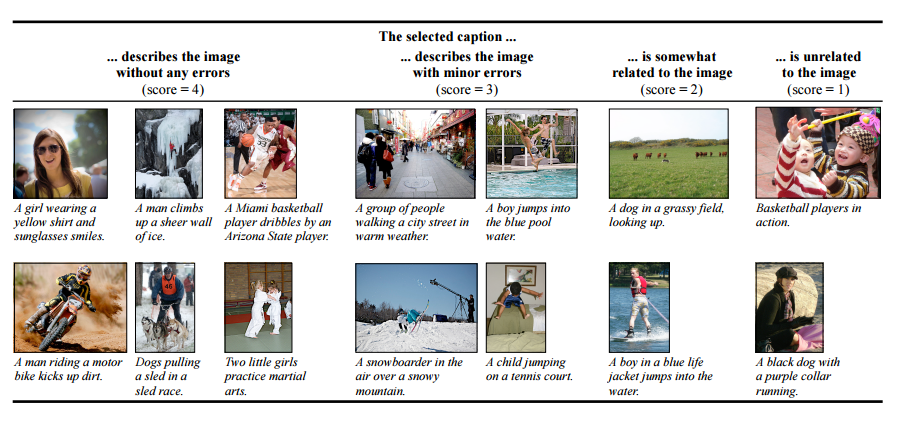
\includegraphics[scale=0.55]{Imgs/sentence_knn1.png}
\caption{نتایج کیفی اختصاص جملات و تصاویر به یک‌دیگر با استفاده از روش نزدیک‌ترین همسایه \cite{hodosh2013framing}}
\label{fig:knn1}
\end{figure}

به علاوه، جدول 
\ref{tbl:knn1}
نتایج ارزیابی روش نزدیک‌ترین همسایه را در اختصاص جملات و تصاویر به یک‌دیگر بر اساس سه معیار نمایش می‌دهد. معیار اول، میانگین امتیازی که افراد خبره به 1000 جملات تولید شده برای هر عکس داده‌اند را نمایش می‌دهد. این امتیازها اعداد صحیح بین ۱ تا ۴ را شامل می‌شوند و بیشینه ممکن برای این معیار، ۴ است. امتیاز بالاتر نشان‌دهنده مناسب‌تر بودن جملات تولید شده هستند. معیارهای \lr{BLUE} و \lr{ROUGE} معیارهایی هیتند که در پژوهش‌های ترجمه ماشین به عنوان محکی برای میزان خوب بودن ترجمه تولید شده، استفاده می‌شوند. مقادیر بالاتر در این معیارها، مناسب بودن عملکرد را نمایش می‌دهد. 

\begin{table}[h]
\center
\caption{نتایج استفاده از روش نزدیک‌ترین همسایه در اختصاص جملات و تصاویر \cite{hodosh2013framing}}
\label{tbl:knn1}
\begin{tabular}{c | c | c }
امتیاز افراد خبره & \lr{BLUE} & \lr{ROUGE}
\\
\hline
\hline
1.57 & 0.35 & 0.11\\
\end{tabular}
\end{table}

به عنوان یکی دیگر از روش‌های مورد استفاده در تولید خودکار شرح بر تصاویر، می‌توان به پژوهش ارائه شده در \cite{kuznetsova2012collective} اشاره کرد. در این پژوهش، تصاویر موجود در مجموعه‌داده، هر کدام با تعدادی عبارت زبانی که توسط کاربران انسانی نوشته شده‌اند، توصیف شده‌اند. در این پژوهش، هدف اصلی این است که با استخراج شبیه‌ترین عبارات موجود در مجموعه‌داده به تصویر ورودی و با کنارهم قرار دادن این عبارات و ساخت جمله با استفاده از چارچوب کاری مورد استفاده در پژوهش‌های تولید زبان طبیعی، جمله متناسب، تولید و نمایش داده‌شود.
\\
علاوه بر استفاده از روش نزدیک‌ترین همسایه برای انتخاب بهترین عبارات زبانی توصیف‌کننده تصویر، می‌توان از استفاده هوشمندانه از مرحله «برنامه‌ریزی محتوا»\enfootnote{Content Planning} در این پژوهش، به عنوان یکی از نقاط قوت آن، یاد کرد. این کار باعث می‌شود علاوه بر تولید جملات سازگار با یک‌دیگر، از تولید جملات تکراری در یک شرح بر یک تصویر، خودداری شود که از نقاط قوت این روش است. این مرحله با استفاده از روش‌های بهینه‌سازی انجام می‌شود. روش برنامه‌سازی خطی صحیح\enfootnote{Integer Linear Programming (ILP)}، به عنوان چارچوب کاری در این مرحله مورد استفاده قرار گرفته است.
\\
در این پژوهش، 89 کلاس از اجسام و 26 کلاس صحنه برای تشخیص محتوا انتخاب شده و تصاویر ورودی، با استفاده از آشکارکننده‌های فلزنسوالب، به این دسته‌ها اختصاص داده می‌شوند. این ‌کار، تخمین مناسبی از محتوای جملات ارائه می‌دهد. همین‌طور با استفاده از روش برچسب‌گذاری نقش کلمات در جمله\enfootnote{Part of Speech Tagging (POS Tagging)}، محتوای عبارات زبانی متناظر با جملات، به طریق مشابه، دسته‌بندی می‌شود.
\\
چهار دسته از عبارات برای هر تصویر ورودی، به این روش، استخراج می‌شود.

\begin{enumerate}
\item عبارات اسمی
\\
جستجوی عبارات اسمی موجود در مجموعه‌داده با استفاده از ویژگی بافت و رنگ به عنوان معیارهای محاسبه شباهت.
\\
مانند:
\begin{center}
\lr{
"The brown cow"
}
\end{center}
\item عبارات فعلی
\\
استفاده از معیارهای مشابه با عبارات اسمی در بین عبارات فعلی موجود در مجموعه‌داده
\\
مانند:
\begin{center}
\lr{
"boy running"
}
\end{center}
\item \enfootnote{Region/Stuff Prepositional Phrases}عبارات اضافی نواحی و اجسام
\\
جستجوی عبارات با استفاده از معیارهای شباهت رنگ، بافت، هیستوگرام گرادیان\enfootnote{Histogram of Gradient (HOG)} و همین‌طور با درنظر گرفتن ویژگی‌های هندسی اجسام
\\
مانند:
\begin{center}
\lr{
"in the sky" , "on the road"
}
\end{center}
\item عبارات اضافی صحنه\enfootnote{Scene Prepositional Pharases}
\\
جستجوی عبارات با استفاده از نتیجه دسته‌بندی صحنه با معیار $L^2$
\\
مانند:
\begin{center}
\lr{
"at the market" , "on hot summer day" , "in Sweden"
}
\end{center}
\end{enumerate}

 هر جمله شامل یک عبارت اسمی، بیان‌کننده مفعول جمله و یک یا چند نمونه از عبارتت دیگر بیان‌کننده مفهوم تصویر هستند. چهار نوع عملیات انتزاعی زیر برای ساخت جمله، در نظر گرفته شده است. هر یک از اعمال زیر با استفاده از روش برنامه‌سازی خطی صحیح، انجام می‌شوند.
 
\begin{enumerate}
 \item انتخاب مجموعه مفعولی که نیاز به توصیف دارند (هر مفعول برای یک جمله)
 \item بازچینی و ترتیب‌دهی به مفعول‌ها
 \item انتخاب مجموعه‌ عبارات مورد نیاز برای هر جمله
 \item بازچینی و ترتیب‌دهی عبارات در هر جمله
\end{enumerate}

در شکل \ref{fig:knn2}، نتایج عملکرد الگوریتم را در مقایسه با جملات تولید شده توسط انسان، مشاهده می‌نمایید. مواردی که با عبارت \lr{ILP} مشخص شده‌اند، خروجی‌های روش برنامه‌سازی خطی صحیح و مواردی که با عبارت \lr{HMM} نمایش داده شده‌اند، جملات تولید شده توسط انسان را نمایش می‌دهند.

\begin{figure}[H]
\center
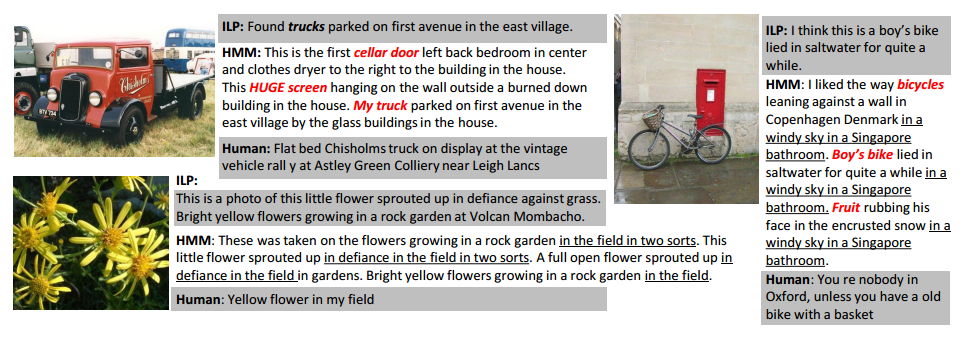
\includegraphics[scale=0.5]{Imgs/sentence_knn2.png}
\caption{نتایج برنامه‌سازی خطی صحیح در مقایسه با جملات تولید شده انسان \cite{kuznetsova2012collective}}
\label{fig:knn2}
\end{figure}

به علاوه، در شکل \ref{fig:knn3}، مواردی را مشاهده می‌نمایید که در آن‌ها، خروجی الگورتیم نسبت به جملات تولید شده توسط انسان، برتری دارد.


\begin{figure}[H]
\center
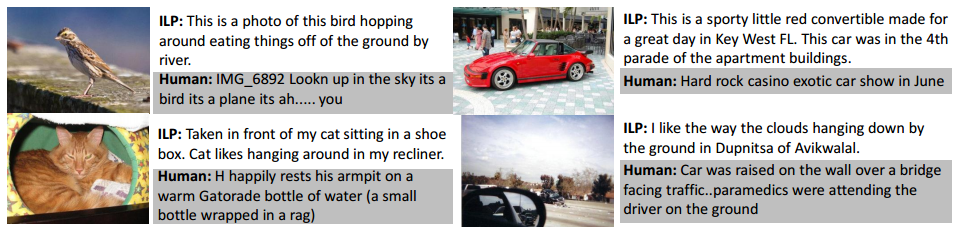
\includegraphics[scale=0.5]{Imgs/sentence_knn3.png}
\caption{مواردی از خروجی برنامه‌سازی خطی صحیح که نسبت به جملات انسان، برتری دارد \cite{kuznetsova2012collective}.}
\label{fig:knn3}
\end{figure}

با وجود این‌که الگوریتم در برخی موارد کارایی بهتری از خود نشان داده‌ است، جملاتی نیز وجود دارند که به لحاظ دستور زبان، عدم شناخت صحیح یا ناسازگاری محتوایی دچار مشکل شده‌اند. شکل \ref{fig:knn4}، نمونه‌هایی از این دست را نمایش می‌دهد.


\begin{figure}[H]
\center
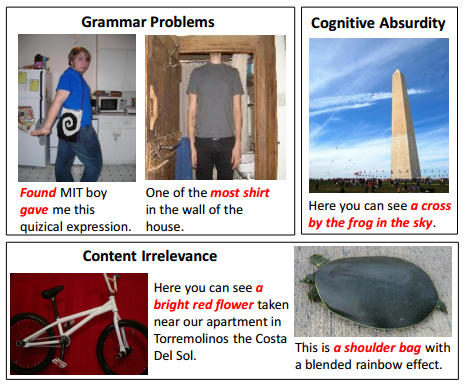
\includegraphics[scale=0.6]{Imgs/sentence_knn4.png}
\caption{نتایج برنامه‌سازی خطی صحیح که به لحاظ‌های مختلف دچار مشکل شده‌اند \cite{kuznetsova2012collective}.}
\label{fig:knn4}
\end{figure}

%%%%%%%%%%%%%%%%%%%%%%%%%%%%%%%%%%%%%%%%%%%%%%%%%%%%%%%%%%
\subsection{استفاده از قالب‌های آماده زبانی}

یکی دیگر از روش‌هایی که برای تولید جمله متناظر با یک تصویر مورد استفاده قرار می‌گیرد، روش استفاده از قالب‌های آماده زبانی است. پژوهش‌هایی که از این روش برای تولید جملات زبانی استفاده کرده‌اند، غالبا پژوهش‌های وظیفه‌‌محور\enfootnote{Task-Based} هستند. حملات تولید شده در این پژوهش‌ها عموما به طور هدف‌مند برای پاسخ دادن به موارد معینی تولید می‌شوند و قابلیت تعمیم‌پذیری کم‌تری نسبت به روش‌های دیگر دارند.
\\
به عنوان مثال در پژوهش \cite{gupta2012image}، یک روش مبتنی بر استفاده از قالب‌های آماده زبانی برای تولید خودکار شرح بر تصاویر ارائه شده است. جملاتی که در این پژوهش تولید می‌شوند، باید قادر به مشخص کردن اطلاعات زیر برای هر تصویر باشند:
\begin{enumerate}
\item اجسامی که در تصویر مشاهده می‌شوند
\item ويژگی‌های اجسام شامل رنگ، اندازه و موارد مشابه
\item فاعل
\item فعل
\item حروف اضافه
\end{enumerate}

در این پژوهش، هدف اصلی این است که پس از برجسب‌زدن تصویر با استفاده از روش‌‌های موجود در حاشیه‌نویسی تصویر\enfootnote{Image Annotation}، که در آن‌ها هر تصویر با یک یا چند برچسب زبانی حاشیه نویسی می‌شود، بتوان جمله‌های بیان‌کننده موارد فوق را در تصویر با استفاده از برچسب‌های تولید شده، تولید نمود.
در این پژوهش از مجموعه‌داده \lr{PASCAL}\enfootnote{\url{http://vision.cs.uiuc.edu/pascal-sentences/}{http://vision.cs.uiuc.edu/pascal-sentences/}} استفاده شده است که شامل 1000 تصویر و برای هر تصویر، ۵ جمله تولید شده توسط انسان است. 
\\
ابتدا با استفاده از یک ابزار برچسب‌زنی نقش کلمات در جملات، تمام کلمات موجود در جملات مجموعه‌داده، برچسب‌ زده می‌شوند. سپس برای هر تصویر، ۲ مفعول از بین ۵ جمله متناظر آن و برای هر مفعول، یک ویژگی استخراج می‌شود. به علاوه با استفاده از نرم‌افزار \lr{WordNet}، مترادف‌های هر یک از کلمات استخراج شده، تا ۳ سطح، یافت می‌شوند.
\\
در مرحله بعدی برای یافتن فاعل جمله، کافیست تعداد دفعاتی را که هر یک از ۲ مفعول استخراج شده، در بین 5 جمله موجود، در نقش فاعل بوده‌اند شمرده و کلمه‌ای را که بیشترین تعداد تکرار به عنوان فاعل را داشته است، به عنوان فاعل جمله در نظر بگیریم. با مشخص شدن فاعل و مفعول جمله، کافیست فعل مورد نظر را با شمارش تعداد دفعات تکرار افعال مختلف در جملاتی که فاعل و مفعولشان برابر با مورد در حال بررسی است، فعل با بیشترین تکرار را انتخاب کنیم. اگر چنین فعلی یافت نشد، از فعل در قالب آماده استفاده نخواهد شد.
\\
موارد مورد نیاز دیگر نیز به همین ترتیب استخراج می‌شوند. در انتها، با توجه به پیدا شدن یا نشدن فعل و همین‌طور نوع فعل استخراج شده، از یکی از قالب‌های زیر برای ساخت جمله استفاده می‌شود.
\begin{enumerate}
\item فعل اصلی استخراج شده است:
\begin{center}
(معرف ۱ - ویژگی ۱ - فاعل) - فعل - حرف اضافه - (معرف ۲ - ویژگی ۲ - مفعول)
\end{center}
\item فعل گذرا استخراج شده است:
\begin{center}
(معرف ۱ - ویژگی ۱ - فاعل) - فعل - (معرف ۲ - ویژگی ۲ - مفعول)
\end{center}
\item فعلی یافت نشده است:
\begin{center}
(معرف ۱ - ویژگی ۱ - فاعل) - حرف اضافه - (معرف ۲ - ویژگی ۲ - مفعول)
\end{center}
\end{enumerate}

شکل \ref{fig:temp1} مواردی از جملات تولید شده برای تصاویر موجود در مجموعه‌داده را نمایش می‌دهد. نمونه‌هایی که در این شکل مشاهده می‌شود، نمونه‌هایی هستند که به لحاظ معنایی صحیح بوده و با تصویر مربوطه سازگاری دارند.

\begin{figure}[H]
\center
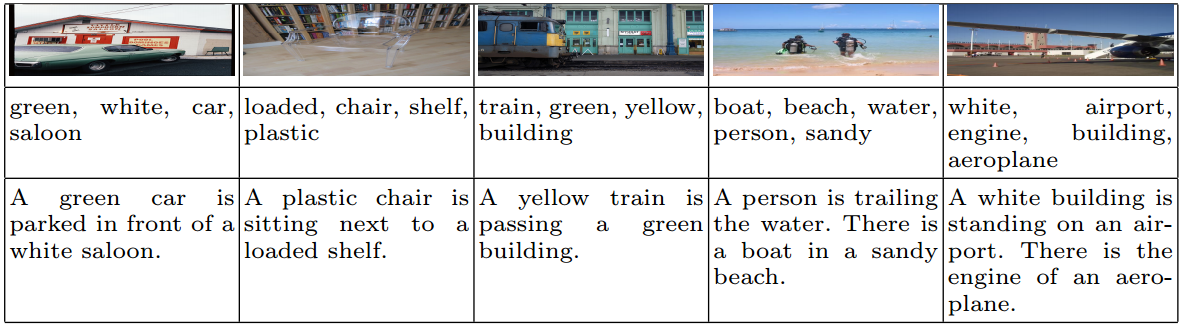
\includegraphics[scale=0.4]{Imgs/sentence_template1.png}
\caption{نمونه‌های صحیح از جملات تولید شده توسط قالب‌های آماده زبانی\cite{gupta2012image}}
\label{fig:temp1}
\end{figure}

به علاوه در شکل \ref{fig:temp2}، نمونه‌هایی از خروجی الگوریتم را در حالاتی که جملات تولید شده به لحاظ شناخت صحیح فاعل، ویژگی، فعل، حروف اضافه و همین‌طور تکرار کلمات در جمله دچار مشکل شده‌اند، نمایش می‌دهد.

\begin{figure}[H]
\center
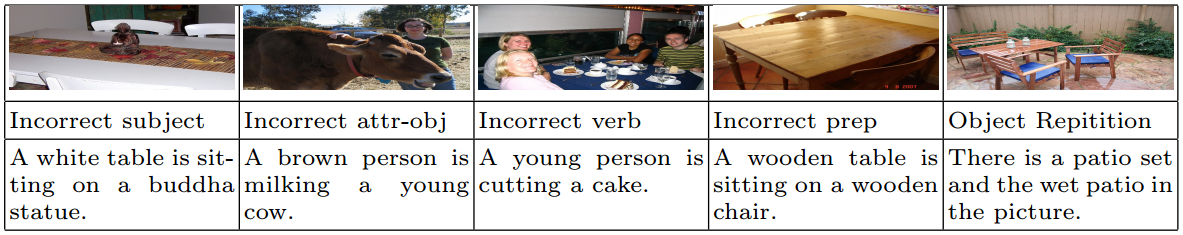
\includegraphics[scale=0.4]{Imgs/sentence_template2.png}
\caption{نمونه‌های اشتباه تولید شده توسط قالب‌های آماده زبانی\cite{gupta2012image}}
\label{fig:temp2}
\end{figure}

علاوه بر این، جدول \ref{tbl:temp1}، نتایج معیار \lr{BLUE} را در حالات مختلف (استفاده از ترکیبات چندتایی کلمات\enfootnote{n-grams}) نمایش می‌دهد. همان‌طور که مشاهده می‌شود، مقادیر به‌دست آمده از این معیارها، قابل قبول بودن دقت جملات تولید شده توسط این روش را نمایش می‌دهند. در ستون‌هایی از جدول که از حرف \lr{s} استفاده شده، تطابق بین کلمات هم‌معنی نیز در نظر گرفته شده است در صورتی‌که در بقیه ستون‌ها، کلمات دقیق با هم مقایسه شده‌اند. همان‌طور که مشخص است، استفاده از کلمات هم‌معنی نتایج بهتری را ارائه داده است.

\begin{table}[H]
\center
\caption{نتایج معیارهای \lr{BLUE} و \lr{ROUGE} درحالات مختلف \cite{gupta2012image}}
\label{tbl:temp1}
\begin{tabular}{c | c | c | c | c | c | c | c}
\lr{BLUE-1} & \lr{BLUE-1-s} & \lr{BLUE-2} & \lr{BLUE-2-s} & \lr{BLUE-3} & \lr{BLUE-3-s} & \lr{ROUGE-1} & \lr{ROUGE-1-s} 
\\
\hline
\hline
0.74 & 0.79 & 0.55 & 0.61 & 0.35 & 0.42 & 0.55 & 0.60 \\
\end{tabular}
\end{table}

%%%%%%%%%%%%%%%%%%%%%%%%%%%%%%%%%%%%%%%%%%%%%%%%%%%%%%%%%%%
%\subsection{روش‌های مبتنی بر مدل‌های آماری}
%
%%%%%%%%%%%%%%%%%%%%%%%%%%%%%%%%%%%%%%%%%%%%%%%%%%%%%%%%%%%
%\subsection{روش‌های صوری}
%
%%%%%%%%%%%%%%%%%%%%%%%%%%%%%%%%%%%%%%%%%%%%%%%%%%%%%%%%%%
\subsection{روش‌های مبتنی بر شبکه‌های عصبی بازگشتی}
اخیرا، استفاده از شبکه‌های عصبی بازگشتی برای تولید جمله، توجه تعداد زیادی از پژوهش‌گران را به خود جلب کرده است. شبکه‌های عصبی بازگشتی، ضمن اثبات قدرت خود در پیش‌بینی سری‌های زمانی، در کاربردهای متعدد و متنوعی مورد استفاده قرار می‌گیرند. از جمله این کاربردها می‌توان به تولید تصاویر، تولید متن، تولید برنامه، تولید موسیقی و مواردی از این دست اشاره نمود. با توجه به ظرفیت بالا و توان یادگیری بالای این مدل‌ها، استفاده از آن‌ها در تولید جملات زبان طبیعی مرتبط با مفهوم یا مفاهیمی خاص، نظر بسیاری را به خود جلب کرده است.
\\
شبکه‌های عصبی بازگشتی در اواخر دهه 1990، ارائه شدند و فعالیت‌های محدودی بر روی مدل‌های کوچکی از ‌آن‌ها مانند مدل \lr{Elman} انجام شد. به دلیل زمان بالای مورد نیاز برای آموزش این نوع از شبکه‌های عصبی، تا سال 2011، عموم فعالیت‌ها در این زمینه، محدود به استفاده از مدل‌های کوچک از این شبکه‌ها بودند. در سال 2011، آقای هینتون\enfootnote{Hinton} و همکارانش در پژوهش \cite{sutskever2011generating}، با بهره‌گیری از پیشرفت‌های جدید در بهینه‌سازی روش بدون هسین\enfootnote{Hessian Free (HF)} و اعمال این روش‌ها به فرایند تولید جمله در سطح حروف\enfootnote{Character Level Sentence Generation} قادر به آموزش یک شبکه عصبی بازگشتی در 5 روز شدند و نتایج بهتری نسبت به مدل‌های ارائه شده تا آن زمان، حاصل کردند.
\\
در پژوهش \cite{sutskever2011generating}، علاوه بر ارائه یک روش برای آموزش شبکه‌های عصبی بازگشتی عمیق بر مبنای روش بهینه‌سازی بدون هسین، نشان داده شده است که شبکه‌های عصبی بازگشتی استاندارد، عملکرد خوبی در تولید جملات در سطح حروف از خود نشان نمی‌دهند. برای حل این مساله، نوع خاصی از این شبکه‌ها موسوم به شبکه‌های عصبی بازگشتی عمیق ضربی\enfootnote{Multiplicative Recurrent Neural Networks (MRNN)} ارائه شده‌اند.
\\
نکات جالبی که در نتایج شبکه عصبی بازگشتی ارائه شده در این پژوهش به چشم می‌خورد، عبارتند از:
\begin{enumerate}
\item تولید ساختارهای زبانی سطح بالا\enfootnote{High level linguistic structures}
\item پشتیبانی از دایره لغات بسیار وسیع
\item یادگیری تعداد قابل توجهی از دستورات زبانی
\item تولید تعداد زیادی اسم محتمل که در بین لغات مجموعه‌داده وجود ندارند
\item توانایی باز و بسته کردن صحیح پرانتزها و نقل قول‌ها در فواصل طولانی بیشا ز 30 حرف
\end{enumerate}

یک شبکه عصبی بازگشتی را که دنباله زمانی $(x-1 \cdots x_T)$ را به عنوان ورودی گرفته و دنباله $(h_1 \cdots h_T)$ و دنباله $(o_1 \cdots o_T)$ را به ترتیب به عنوان حالات مخفی و خروجی، تولید می‌کند می‌توان مطابق با رابطه 
\ref{eq:rnn1}
بیان کرد. در این رابطه، $W_{hx}$ ماتریس وزن‌های لایه ورودی به لایه مخفی، $W_{hh}$ ماتریس وزن‌های لایه مخفی به لایه مخفی (وزن‌های بازگشتی) و $W_{oh}$ ماتریس وزن‌های لایه مخفی به لایه خروجی است. بردارهای $b$، بردارهای بایاس هستند و مقدار $W_{hh}h_{t-1}$ در نقطه $t = 1$ با یک مقدار اولیه جایگزین می‌شود.

\begin{align*}
h_t &= tanh(W_{hx}x_t + W_{hh}h_{t-1} + b_h) 
\\
o_t &= W_{oh}h_t + b_o
\numberthis
\label{eq:rnn1}
\end{align*}

از آنجا که مشتقات رابطه \ref{eq:rnn1} قابل محاسبه هستند، به راحتی می‌توان رابطه به‌روزرسانی وزن‌ها را بر اساس روش نزول در امتداد گرادیان، برای شبکه عصبی بازگشتی، محاسبه کرد. با این وجود، به دلیل رابطه بین پارامترها و دینامیک شبکه، روش نزول در امتداد گرادیان کارایی خوبی در آموزش شبکه برای پیش‌بینی دنباله‌های زمانی در بازه‌های زمانی بزرگ، ارائه نمی‌دهد. به همین دلیل، تا سال 2011 و ارائه روش بهینه‌سازی بدون هسین در \cite{sutskever2011generating} برای آموزش شبکه عصبی بازگشتی، پژوهش‌های زیادی در این زمینه انجام نمی‌شد.
\\
برای رفع مشکل روش پس‌انتشار خطا\enfootnote{Backpropagation} در آموزش شبکه‌های عصبی بازگشتی، سه روش زیر پیشنهاد شده است:
\begin{enumerate}
\item استفاده از شبکه‌های عصبی حالت پژواک\enfootnote{Echo State Network}
\\
در این شبکه‌ها، فقط وزن‌های پیش‌رو\enfootnote{Feed forward}‌ به روزرسانی می‌شوند. مقادیر اولیه برای وزن‌های بازگشتی باید به طور مناسب انتخاب شوند.
\item شبکه‌های حافظه کوتاه‌مدت بلند\enfootnote{Long Short Term Memory (LSTM)}
\\
در این شبکه‌ها، گره‌هایی برای به‌خاطر سپاری ورودی‌های قدیمی تعبیه می‌شود که باعث افزایش قدرت این شبکه‌ها در پیش‌بینی بلندمدت دنباله‌های زمانی می‌شود.
\item استفاده از بهینه‌سازی بدون هسین در آموزش شبکه‌های عصبی بازگشتی ضربی
\\
این مدل، تاکنون توانسته کارایی بهتری از هر دو مدل قبلی از خود نشان دهد \cite{sutskever2011generating}.
\end{enumerate}

در ادامه به بررسی شبکه عصبی ارائه شده در پژوهش \cite{sutskever2011generating} می‌پردازیم.

\subsubsection[شبکه عصبی بازگشتی ضربی]{شبکه عصبی بازگشتی ضربی\cite{sutskever2011ge3nerating}}

ایده اصلی در طراحی این شبکه این است که به جای استفاده و آموزش یک ماتریس یکسان از وزن‌های لایه مخفی به ازای تمام ورودی‌های ممکن، به ازای هر ورودی ممکن، یک ماتریس وزن داشته باشیم. به عبارت دیگر، هر حرفی که به عنوان ورودی به شبکه وارد شد، مشخص کننده ماتریسی باشد که به عنوان وزن‌های لایه مخفی در آموزش شبکه شرکت می‌کند. با این ایده، رابطه \eqref{eq:rnn1} به شکل رابطه \eqref{eq:rnn2} تبدیل می‌شود. 

\begin{align*}
h_t &= tanh(W_{hx}x_t + W_{hh}^{(x_t)}h_{t-1} + b_h) 
\\
o_t &= W_{oh}h_t + b_o
\numberthis
\label{eq:rnn2}
\end{align*}

همان‌طور که ملاحظه می‌شود، تنها تفاوت رابطه 
\eqref{eq:rnn1}
 و رابطه 
 \eqref{eq:rnn2}
  در بالانویس پارامتر 
 $W_{hh}$
  است. پارامتر جدید را می‌توان به شکل رابطه 
 \eqref{eq:rnn3}
  تعریف کرد که در آن، 
  $x_t^{(m)}$
   مولفه
   $m$
   ام از ورودی
  $x_t$
   و 
  $W_{hh}^{(m)}$
   است. لازم به ذکر است در رابطه
    \eqref{eq:rnn3}
     برای تعریف 
   $W_{hh}^{(x_t)}$ 
   از تنسور
   \enfootnote{Tensor}
    استفاده شده است. در این میان،
     $M$
      تعداد ابعاد ورودی 
     $x_t$
      و ماتریس‌های 
     $W_{hh}^{(1)}$
      تا 
     $W_{hh}^{(M)}$
      ماتریس‌های 
مربوط به هریک از ابعاد ورودی هستند.

\begin{equation}
W_{hh}^{(x_t)} = \ML{\Sigma}_{m = 1}^M x_t^{(m)}W_{hh}^{(m)}
\label{eq:rnn3}
\end{equation}

مدل ارائه شده از آنجا که به طور کامل عمومی است، در حالاتی که ابعاد ورودی و تعداد گره‌های مخفی زیاد باشد، دچار مشکل می‌شود زیرا حجم زیادی حافظه نیاز خواهد داشت. برای حل این مشکل، سعی در فاکتورگیری از پارامتر $W_{hh}^{(x_t)}$ خواهیم داشت.
\\
با تعریف سه ماتریس 
$W_{hf}$
، $W_{fh}$ و $W_{fx}$ و تغییر رابطه \eqref{eq:rnn3} به شکل رابطه \eqref{eq:rnn4}، می‌توان این فاکتورگیری را تعریف کرد.

\begin{equation}
W_{hh}^{(x_t)} = W_{hf} \cdot diag(W_{fx}x_t) \cdot W_{fh}
\label{eq:rnn4}
\end{equation}

در صورتی‌که ابعاد ماتریس $W_{fx}x_t$ که آن را $F$ خواهیم نامید، بزرگ باشد، رابطه \eqref{eq:rnn4} به همان اندازه رابطه \eqref{eq:rnn3} پیچیده خواهد بود اما در صورتی‌که این ابعاد کوچک باشد، رابطه \eqref{eq:rnn4} نسبت به رابطه \eqref{eq:rnn3} به مراتب ساده‌تر خواهد بود. با جای‌گذاری رابطه \eqref{eq:rnn4} در رابطه \eqref{eq:rnn2}، شبکه عصبی بازگشتی ضربی به‌دست خواهد آمد. رابطه نهایی را می‌توان به شکل رابطه \eqref{eq:rnn5} نمایش داد.

\begin{align*}
f_t &= diag(W_{fx}x_t) \cdot W_{fh}h_{t-1}
\\
h_t &= tanh(W_{hf}f_t + W_{hx}x_t)
\\
o_t &= W_{oh}h_t + b_o
\numberthis
\label{eq:rnn5}
\end{align*}

شکل \ref{fig:rnn1}
طرح‌واره‌ای از مدل کلی شبکه عصبی بازگشتی ضربی را که توسط رابطه \eqref{eq:rnn5} مدل شده است، نمایش می‌دهد. علامت مثلث که در شکل نشان داده شده است، نمایش‌دهنده یک گیت\enfootnote{Gate} را نمایش می‌دهد که در آن، وزن لایه مخفی با استفاده از ورودی، انتخاب می‌شود.

\begin{figure}[H]
\center
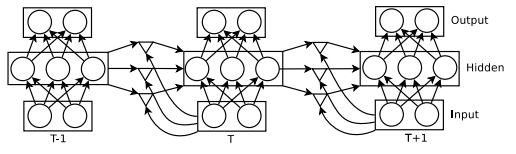
\includegraphics[scale=0.8]{Imgs/sentence_rnn1.png}
\caption{طرح‌واره شبکه عصبی بازگشتی ضربی \cite{sutskever2011generating}}
\label{fig:rnn1}
\end{figure}

نکته‌ای که هم‌چنان مبهم باقی می‌ماند، نحوه محاسبه وزن‌های مخفی است. رابطه \eqref{eq:rnn6} نحوه محاسبه $W_{hh}^{(x_t) ij}$ را نمایش می‌دهد. در این حاصل‌ضرب، اگر به عنوان مثال پارامتر $W_{hh if}$ خیلی کوچک باشد و $W_{hh fj}$ خیلی بزرگ باشد یا برعکس، حاصل مشتق، برای وزن‌های بسیار کوچک، بسیار بزرگ می‌شود و برای وزن‌های بسیار بزرگ، بسیار کوچک. این باعث می‌شود روش نزول در امتداد گرادیان، به حالت پایداری نرسد.

\begin{equation}
W_{hh}^{(x_t) ij} = \ML{\Sigma}_f W_{hh if}W_{hh fx^t}W_{hh fj}
\label{eq:rnn6}
\end{equation}

به دلیل همین عدم پایداری ایجاد شده، حاصل از رابطه \eqref{eq:rnn6}، روش نزول در امتداد گرادیان، گزینه‌ مناسبی برای آموزش این شبکه نخواهد بود. لذا لزوم استفاده از روش‌های مرتبه دوم مانند روش بدون هسین، مشهود می‌شود.

\subsubsection{تولید جمله با مفهوم مشخص}
استفاده از شبکه عصبی بازگشتی ضربی منجر به فراهم‌سازی بستری مناسب جهت تولید جمله در سطح حروف می‌شود. با این وجود برای تولید خودکار شرح بر تصاویر، نیازمند آن‌ هستیم که محتوای جملات را به طور مشخص و از پیش تعیین شده داشته باشیم. به همین دلیل نیاز به ارائه روش که طی آن بتوانیم معنا و محتوای جملات تولید شده توسط شبکه عصبی بازگشتی را کنترل کنیم، مشهود می‌شود.
\\
در پژوهش \cite{karpathy2015deep} روش جدیدی برا تولید شرح خودکار بر تصاویر ارائه شده است که در مرحله تولید جمله، از نوع خاصی از شبکه‌های عصبی بازگشتی موسوم به شبکه عصبی بازگشتی دوطرفه\enfootnote{Bidirectional RNN}، استفاده  شده است. در این روش، ابتدا از یک شبکه عصبی کانولوشنی عمیق بر روی نواحی استخراج شده از تصاویر برای استخراج ویژگی و درک صحنه استفاده شده است. از سوی دیگر، با اعمال یک شبکه عصبی بازگشتی دوطرفه بر جملات و ارائه یک تابع هدف ساختارمند، روشی برای هم‌ترازسازی جمله و اطلاعات بصری نهفته در تصویر ارائه شده است.
\\

شکل \ref{fig:deep1}، نمونه‌ای از هم‌ترازسازی ارائه شده در این پژوهش برای یک تصویر را نشان می‌دهد.
\begin{figure}[H]
\center
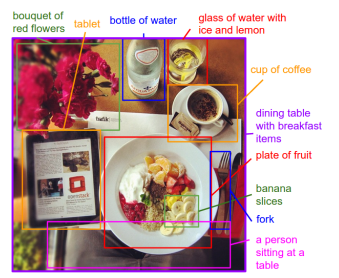
\includegraphics[scale=0.6]{Imgs/sentence_deep1.png}
\caption{هم‌ترازسازی تصویر و جمله\cite{karpathy2015deep}}
\label{fig:deep1}
\end{figure}

در مدل هم‌ترازسازی ارائه شده در این پژوهش، فرض بر این است که یک مجموعه‌داده شامل تعداد زیادی تصویر و جملات متناظر با هر تصویر وجود دارد. همین‌طور فرض دیگری وجود دارد مبنی بر این‌که بخش‌های مختلف هر جمله، به نواحی خاصی از تصویر اشاره‌ می‌کنند که موقعیت این نواحی مجهول است. از طرف دیگر اشاره این بخش‌ها به نواحی مرتبط خود در تصاویر، در بین تمام مجمو‌‌عه‌داده، تکرار می‌شود. به عنوان مثال، عبارات زبانی شامل کلمه «توپ» در تمام تصاویر موجود در مجموعه‌داده، به نواحی از تصویر اشاره می‌کنند که دارای ويژگی‌های «توپ» هستند.
\\
در شکل \ref{fig:deep2} ارتباط بین بخش‌های مختلف یک جمله و نواحی متفاوت از تصویر را مشاهده می‌نمایید. همان‌طور که در شکل مشاهده می‌شود، ابتدا برای تصاویر موجود در مجموعه‌داده و شرح متناظر با هر یک از این تصاویر، ارتباطات بین عبارات مختلف از جملات و نواحی تصاویر استخراج و یادگرفته می‌شود. در ادامه، با ورود یک  تصویر جدید و براساس ارتباطات یادگرفته شده، شرح جدید برای تصویر تولید می‌شود.

\begin{figure}[H]
\center
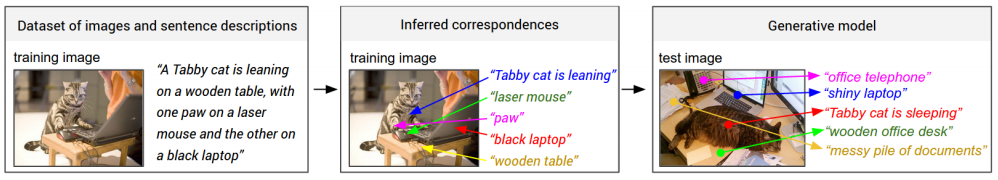
\includegraphics[scale=0.45]{Imgs/sentence_deep2.png}
\caption{ارتباط بین نواحی مختلف یک تصویر و عبارات جمله\cite{karpathy2015deep}}
\label{fig:deep2}
\end{figure}

برای تبدیل تصویر به فضای ویژگی، مطابق با آن‌چه در فصل درک صحنه ذکر شد، ابتدا با استفاده از روش شبکه‌های عصبی کانولوشنی ناحیه‌ای،‌ ۱۹ ناحیه از تصویر استخراج شده و برای ۲۰ تصویر موجود، با اعمال یک بهینه‌سازی و تخمین پارامتر و اعمال یک شبکه عصبی، بردار ویژگی استخراج می‌شود. پس از استخراج بردار ویژگی از نواحی تصویر، نیازمند آن هستیم که بتوانیم از عبارات مختلف جمله، بردار ویژگی هم‌اندازه با بردار ویژگی حاصل از تصویر، استخراج کنیم. برای این کار، در این پژوهش از شبکه‌ عصبی بازگشتی دوطرفه استفاده شده است. 
\\
این شبکه عصبی، یک دنباله از $N$ کلمه را به عنوان ورودی دریافت کرده و هر یک را به یک بردار در فضای $h$ بعدی، که $h$ اندازه بردار ویژگی حاصل از نواحی تصویر است، نگاشت می‌کند. رابطه \eqref{eq:deep1}، رابطه مربوط به پارامترهای این شبکه عصبی را نمایش می‌دهد.
در این رابطه، $I$ یک بردار ستونی اندیکاتور\enfootnote{Indicator} است که در اندیس کلمه $t$ام خود یک و در بقیه اندیس‌ها صفر دارد. $W_w$ یک ماتریس وزن ثابت برای هر کلمه $w$ است که برای جلوگیری از بیش‌برازش بر داده‌ها، مورد استفاده قرار می‌گیرد.

\begin{align*}
x_t &= W_{w} I_t 
\\
e_t &= f(W_ex_t + b_e)
\\
h_t^f &= f(e_t + W_fh_{t-1}^f + b_f)
\\
h_t^b &= f(e_t + W_bh_{t-1}^b + b_b)
\\
s_t &= f(W_d(h_t^f + h_t^b) + b_d)
\numberthis
\label{eq:deep1}
\end{align*}

 در این شبکه، دو جریان داده وجود دارد. جریان اول، جریان داده بین گر‌ه‌های مخفی شبکه از چپ به راست و دیگری جریان داده بین نود‌های مخفی شبکه از راست به چپ است که به ترتیب با $h_t^f$ و $h_t^b$ نمایش داده می‌شوند. بردار نهایی $s_t$، بردار حاصل از نگاشت کلمات به فضای ویژگی‌ها است که با استفاده از خود کلمه و محتوای مورد استفاده در اطراف کلمه در جمله، تولید می‌شود.
\\
شکل \ref{fig:deep3} طرح‌واره‌ای از معماری این شبکه را نمایش می‌دهد. همان‌طور که در این شکل مشخص است، در لایه مخفی این شبکه، دو جریان داده، یکی از راست به چپ و دیگری از چپ به راست برای محاسبه تاثیر کلمات اطراف کلمه جاری بر نگاشت کلمه به فضای ویژگی‌ها، وجود دارد.

\begin{figure}[H]
\center
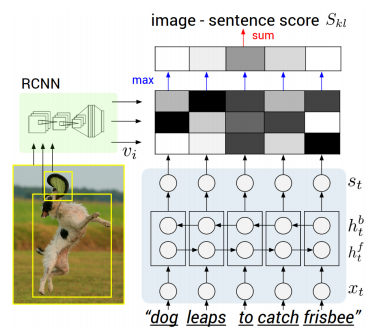
\includegraphics[scale=0.8]{Imgs/sentence_deep3.png}
\caption{طرح‌واره شبکه عصبی بازگشتی دوطرفه\cite{karpathy2015deep}}
\label{fig:deep3}
\end{figure}

 در ادامه با بهره‌گیری از روش نگاشت دوطرفه تصاویر و جملات که در بخش درک صحنه ارائه شد، توابع هم‌ترازسازی و تابع هدف ارائه شده را مورد استفاده قرار داده و با استفاده از روش یادگیری چند نمونه‌ای، اقدام به یادگیری انتساب‌های بین نواحی مختلف تصاویر و عبارات مختلف زبانی می‌شود.
 \\
 با استفاده از این روش، می‌توان برای هر ناحیه از تصویر، کلمات مناسب را تعیین کرد. اما برای تولید خودکار شرح بر تصاویر، نیاز به تولید عبارات زبانی وجود دارد. برای حل این مشکل، با در نظر گرفتن رابطه ضرب داخلی بین بردارهای ویژگی حاصل از نواحی تصویر و عبارات زبانی یک جمله به عنوان معیار شباهت، روشی ارائه شده است که بتوان برای هر ناحیه از تصویر، عبارت زبانی مناسبی تولید کرد.
 \\
 در این روش، با تعریف یک تابع انرژی و استفاده از مدل میدان تصادفی مارکف، با بهینه‌سازی تابع انرژی ارائه شده، بهترین هم‌ترازسازی برای هر یک از عبارات موجود محاسبه شده و عبارت با بهترین مقدار، انتخاب می‌شود. رابطه \eqref{eq:deep2}، این تابع انرژی را محاسبه می‌کند.
 
 
 \begin{align*}
 E(a) =  \ML{\Sigma}_{j=1\cdots N}\Psi_j^U(a_j) &+ \ML{\Sigma}_{j=1\cdots M}\Psi_j^B(a_j, a_{j+1})
 \\
 \Psi_j^U(a_j) &= \nu_i^T \cdot s^t
 \\
 \Psi_j^B(a_j,a_{j+1}) &= \beta I(a_j = a_{j+1})
 \numberthis
 \label{eq:deep2}
 \end{align*}


می‌توان در شکل \ref{fig:deep7} نتایج استفاده از این شبکه و محاسبه میزان شباهت نواحی مختلف تصویر و عبارات مختلف از جملات را مشاهده نمود. این شکل، نتیجه آموزش اختصاص نواحی مختلف تصویر به عبارات زبانی را نمایش می‌دهد.

\begin{figure}[H]
\center
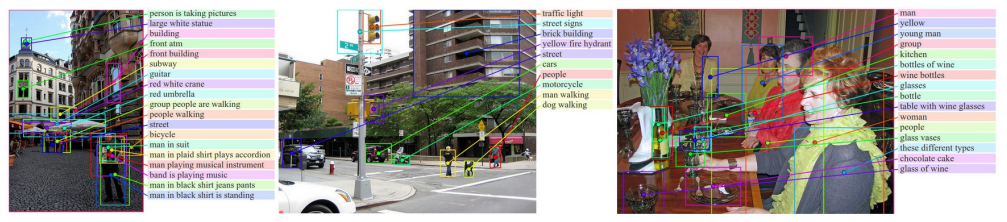
\includegraphics[scale=0.5]{Imgs/sentence_deep7}
\caption{انتساب نواحی مختلف تصویر به عبارات زبانی\cite{karpathy2015deep}}
\label{fig:deep7}
\end{figure}


تا این مرحله، با ورود یک تصویر، یا یک ناحیه از تصویر، عبارات زبانی متناظر، استخراج شده‌اند. هدف اصلی در این پژوهش تولید جمله برای هر تصویر است. بنابراین نیاز داریم تا با استفاده از مدل‌های ارائه شده برای تولید جمله، این کار را انجام دهیم. در پژوهش‌های زیادی، استفاده از شبکه‌های عصبی بازگشتی برای پیش‌بینی و محاسبه توزیع احتمال کلمه بعدی در یک جمله با در نظر داشتن کلمات قبلی و محتوای جمله، ارائه شده است. در این پژوهش با اعمال تغییرات کوچکی، از همین روش‌ها استفاده می‌شود. 
\\
رابطه ارائه شده برای شبکه عصبی بازگشتی که این کار را انجام می‌دهد، مطابق با رابطه \eqref{eq:deep3} است.
در این رابطه، $CNN_{\theta c}(IMAGE)$ بردار حاصل از اعمال آخرین لایه یک شبکه عصبی کانولوشنی بر تصویر را نشان می‌دهد و بقیه پارامترها، همگی قابل آموزش هستند. بردار $y_t$ بردار نماینده توزیع احتمالاتی تمام کلمات با در نظر گرفتن کلمات قبلی و محتوای هر ناحیه است که اندازه آن برابر است با تعداد تمام کلمات موجود در لغت‌نامه به علاوه یک نشانه خاص به عنوان «اتمام جمله».

\begin{align*}
b_\nu &= W_{hi}[CNN_{\theta c}(IMAGE)]
\\
h_t &= f(W_{hx}x_t + W_{hh}h_{t-1} + b_h + I(t = 1)\cdot b_\nu)
\\
y_t &= softmax(W_{oh}h_t + b_o)
\numberthis
\label{eq:deep3}
\end{align*}

شکل \ref{fig:deep4}، طرح‌واره‌ای از شبکه عصبی بازگشتی مالتی‌مودال\enfootnote{Multimodal} ارائه شده در این پژوهش برای تولید جمله را نمایش می‌دهد.

\begin{figure}[H]
\center
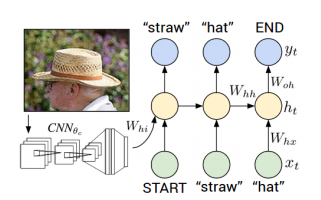
\includegraphics[scale=1]{Imgs/sentence_deep4.png}
\caption{طرح‌واره شبکه عصبی بازگشتی ارائه شده برا تولید جمله\cite{karpathy2015deep}}
\label{fig:deep4}
\end{figure}

جدول \ref{tbl:deep}
نتایج معیار \lr{BLUE} را برای روش ارائه شده بر روی سه مجموعه‌داده مختلف، نمایش می‌دهد. همان‌طور که در این جدول مشخص است، نتایج به دست آمده از این روش در مقایسه با دو روش دیگر، نتایج به نسبت بهتری بوده است.

\begin{table}[H]
\center
\caption{نتایج معیار \lr{BLUE} برای روش ارائه شده در \cite{karpathy2015deep} در مقایسه با دو روش دیگر}
\label{tbl:deep}
\begin{tabular}{c | c | c | c || c | c | c || c | c | c | c}
نام روش
&
\lr{B-1} &\lr{B-2} &\lr{B-3} &
\lr{B-1*} &\lr{B-2*} &\lr{B-3*} &
\lr{B-1**} &\lr{B-2**} &\lr{B-3**} &\lr{B-4**} 
\\
\hline
\hline
نزدیک‌ترین‌همسایه
&
ــ &ــ & ــ &
ــ &ــ & ــ &
45.0 &28.1 &16.6 &10.0
\\
روش \cite{mao2014explain}
&
58 & 28 & 23 &
55 & 24 & 20  &
ــ &ــ &ــ &ــ
\\
روش \cite{karpathy2015deep}
&
57.9 & 38.3 & 24.5 & 57.3 & 36.9 & 24.0 & 62.5 & 45.0 & 32.1 & 23.0 

\end{tabular}

\end{table}


شکل \ref{fig:deep5} نتایج رتبه‌بندی جملات و عبارات برای هر ناحیه از تصویر را نمایش می‌دهد.

\begin{figure}[H]
\center
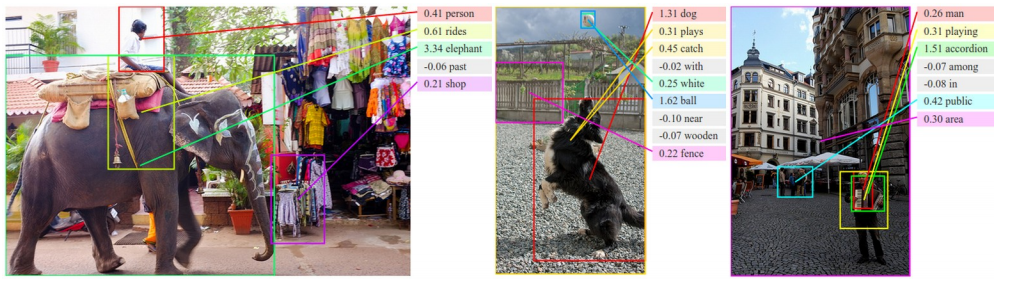
\includegraphics[scale=0.5]{Imgs/sentence_deep5.png}
\caption{نتایج رتبه‌بندی عبارات زبانی برای نواحی تصویر \cite{karpathy2015deep}}
\label{fig:deep5}
\end{figure}

به علاوه، در شکل \ref{fig:deep6} نتایج تولید شرح برای تصاویر، توسط شبکه عصبی بازگشتی ارائه شده در این پژوهش، به تصویر کشیده شده است.

\begin{figure}[H]
\center
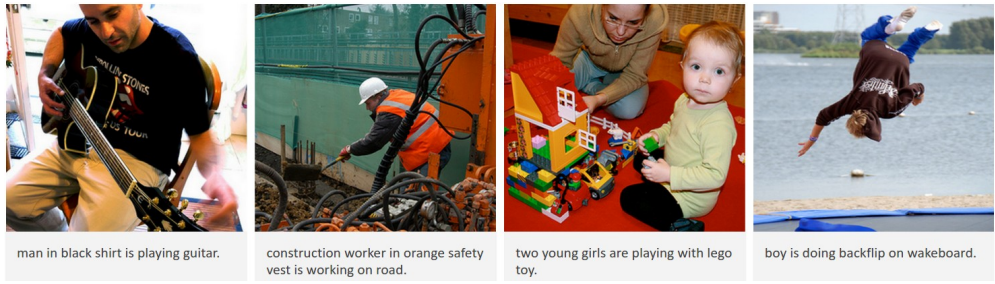
\includegraphics[scale=0.5]{Imgs/sentence_deep6}
\caption{نتایج تولید جمله برای تصاویر در \cite{karpathy2015deep}}
\label{fig:deep6}
\end{figure}



%%%%%%%%%%%%%%%%%%%%%%%%%%%%%%%%%%%%%%%%%%%%%%%%%%%%%%%%%%
\subsection{جمع‌بندی}

چالش تولید جمله یکی از قدیمی‌ترین و پویاترین حوزه‌های فعالیتی و پژوهشی در هوش مصنوعی است که از اواسط قدن بیستم، توجه پژوهش‌گران بسیاری را به خود جلب کرده است. روش‌های مختلفی برای حل این مساله ارائه شده‌اند. از جمله این روش‌ها می‌توان به موارد زیر اشاره کرد:

\begin{enumerate}
\item تولید زبان طبیعی
\\
در این دسته از روش‌ها که از اواخر دهه بیستم تا کنون مورد استفاده قرار می‌گیرند، با طی فرایند در یک چارچوب کلی، سعی در تولید جملات مناسب دارند. این دسته از روش‌ها عموما برای تفسیر خودکار داده‌هایی که برای کاربران انسانی غیر قابل تفسیر هستند یا تفسیر دشواری دارند، به‌کار می‌روند. در این روش‌ها ابتدا با استفاده از ویژگی‌های مختلفی که در داده‌های ماشینی (داده‌های قابل تفسیر برای ماشین) کلمات مناسب انتخاب شده و سپس با استفاده از کلمات منتخب، عبارات زبانی (با جایگشت دادن کلمات و حذف عبارات غیر محتمل) تولید می‌شوند. سپس با اعمال قواعد دستور زبان و چینش عبارات زبانی در کنارهم، جملات نهایی تولید می‌شوند.
\item نزدیک‌ترین همسایه
\\
در این دسته از روش‌ها سعی می‌شود با ورود یک تصویر و نگاشت آن به فضای ویژگی‌ها، جمله‌ای از میان تمام جملات موجود در مجموعه‌داده انتخاب شود که بیشترین مشابهت با بردار ویژگی تصویر را دارد. بزرگ‌ترین مشکل در این روش‌ها انتخاب معیار مناسب برای محاسبه فاصله بین یک جمله و بردار ویژگی حاصل از تصویر است. در این روش، علاوه بر این‌که نیاز به وجود مجموعه‌داده وسیع و پوشا وجود دارد، ممکن است جمله نهایی، در انتها گویا و بیان‌کننده تمام جوانب تصویر نباشد و یا حتی با تصویر ورودی سازگاری نداشته باشد.
\\
برای حل این مشکل، سعی شد به جای استخراج نزدیک‌ترین جمله به تصویر موجود، مشابه‌ترین عبارات زبانی را با شکستن جملات موجود به عبارات سازنده، انتخاب کرده و با بهره‌گیری از روش تولید زبان طبیعی و یا روش‌های دیگر، چینش مناسبی از این عبارات را که در قالب یک یا چند جمله بیان شوند، تولید و به عنوان شرح بر تصویر، نمایش داد.
\item استفاده از قالب‌های زبانی آماده
\\
با وجود فعالیت‌های گوناگون در این زمینه و استفاده از روش‌های مختلف، هم‌چنان تضمین صحت جمله خروجی، کار دشواری است. به همین دلیل، سعی شد با ارائه یک یا چند قالب زبانی آماده و از پیش تعیین شده برای جملات، مانند قالب‌های جملات خبری، صحت جملات نهایی را تضمین کرد. در این دسته از روش‌ها، ویژگی‌های مختلفی از تصویر استخراج می‌شود که هریک از این ویژگی‌ها یا همه آن‌ها در کنار هم قادر هستند نقش‌هایی مانند «فعل»، «فاعل»، «مفعول» و موارد مشابه را در جمله متناظر با تصویر مشخص کنند. با استخراج کلمات مناسب و شناخت نقش آن‌ها در جمله و جای‌گذاری هر یک از این کلمات در مکان مناسب نقشی خود در قالب از پیش تعیین شده، جمله متناظر با هر تصویر استخراج می‌شود.
\item استفاده از شبکه‌های عصبی بازگشتی
\\
اگر چه استفاده از قالب‌های آماده و از پیش تعیین شده، تا حدی مشکلات موجود را حل می‌کند اما هم‌چنان چالش بزرگ‌تری حل نشده باقی مانده است. تولید جملات جدید، استفاده از کلمات و عبارات جدید و ابتکاری به طوری‌که علاوه بر تضمین رعایت دستور زبان، بتوان معنای جمله را نیز متضمن شد، چالش بزرگی است که در این مسیر کماکان وجود دارد.
\\
استفاده از شبکه‌های عصبی بازگشتی یکی از بهترین راه‌کارهای موجود برای حل این مشکل و رویارویی با این چالش هستند. استفاده از این شبکه‌ها در اواخر قرن بیستم در بین پژوهش‌گران رواج پیدا کرد تا جایی که ناپایداری الگوریتم پس‌انتشار خطا در آموزش این شبکه، راه را برای پژوهش‌های بعدی بست. پس از ارائه یک روش مناسب برای بهینه‌سازی بدون هسین در سال 2010، روشی برای آموزش یک شبکه عصبی بازگشتی موسوم به شبکه عصبی بازگشتی ضربی بر مبنای بهینه‌سازهای بدون هسین ارائه شد و نتایج آن به طور چشم‌گیری از روش‌های موجود بیشتر بود.
\\
ارائه شبکه عصبی بازگشتی ضربی، نقطه عطفی در مسیر علم در راستای حل چالش تولید جمله به حساب می‌آید. از حدود سال 2011 به بعد، استفاده از شبکه‌های عصبی بازگشتی برای تولید جمله به پویاترین و پرفعالیت‌ترین حوزه در مسائل مربوط به تولید جمله، به حساب می‌آید.
\end{enumerate}

خانم لی و همکارانش در سال 2015، در پژوهش \cite{karpathy2015deep}، با استفاده از شبکه‌های عصبی کانولوشنی عمیق و دو نوع از شبکه‌های عصبی بازگشتی موسوم به شبکه‌های عصبی بازگشتی مالتی‌مودال و شبکه‌های عصبی بازگشتی دوطرفه، روش مناسبی برای تولید خودکار شرح بر تصاویر ارائه داده است.
\\
در این پژوهش، ابتدا با بهره‌گیری از روش شبکه عصبی کانولوشنی ناحیه‌ای، نواحی از تصویر که شامل تصویر اجسام است، استخراج شده و با استفاده از یک شبکه عصبی کریشفسکی، بردار ویژگی برای هر ناحیه محاسبه می‌شود. سپس با بهره‌گیری از یک شبکه عصبی بازگشتی دوطرفه، عبارات مختلف از جمله استخراج و بردارهای ویژگی برای هر عبارت محاسبه می‌شود. سپس با استفاده از یک تابع هدف و مدل میدان تصادفی مارکف، هم‌ترازسازی بین نواحی و عبارات زبانی صورت گرفته و مدل آموزش داده می‌شود.
\\
 در ادامه با تخمین بهینه پارامترهای موجود و با استفاده از شبکه عصبی بازگشتی مالتی‌مودال، توزیع احتمال بهترین کلمه بعدی در یک جمله با داشتن کلمات قبلی و محتوای حاصل از بردار ویژگی محاسبه شده روی نواحی تصویر، محاسبه شده و بهترین کلمه بعدی تولید می‌شود. این کار تا جایی ادامه می‌یابد که شبکه، نشانه مخصوص پایان جمله را تولید کند.
  
%
%\createTitlePage{فصل چهارم}{ارائه نتایج}
%\createTitlePage{فصل چهارم}{ارائه نتایج}
\subsection{ارائه نتایج}
این فصل در گزارش کامل، تکمیل خواهد شد.
%
\createTitlePage{فصل چهارم}{جمع‌بندی و نتیجه‌گیری}
\subsection{جمع‌بندی و نتیجه‌گیری}


%introduction
در این مستند، گزارش مختصری درباره مساله تولید خودکار شرح بر تصاویر و روش‌های پیشنهادی برای حل چالش‌های موجود در این مسیر را ارائه دادیم. مساله تولید خودکار شرح بر تصاویر، به معنای تولید جملات زبان طبیعی برای هر تصویر است به طوری‌که این جملات شامل سه شرط زیر باشند:
\begin{enumerate}
\item صحنه، اجسام موجود در تصویر، رابطه مکانی اجسام و اطلاعاتی از این دست که به درک تصویر کمک می‌کنند باید در جملات تولید شده وجود داشته باشند و دقیق و کامل باشند.
\item جملات تولید شده، خود، باید به لحاظ معنایی، دستور زبان و املایی صحیح بوده و نقصی نداشته باشند.\
\item جملات تولید شده باید با تصاویر مرتبط با خود، سازگاری داشته باشند.
\end{enumerate}

ایده‌های اولیه در این مسیر از پژوهش‌های موجود در زمینه ترجمه ماشین ایجاد شده است که در آن‌ها، ابتدا یک جمله ورودی از یک زبان مبدا، با استفاده از روش‌های مختلفی به یک بردار ویژگی تبدیل می‌شود و سپس در مرحله دوم، بردار ویژگی حاصل، با استفاده از روش‌های خاص دیگری به جملات زبان طبیعی به زبان مقصد، تبدیل می‌شوند. حال اگر به جای جمله از زبان مبدا، یک تصویر به این سامانه وارد شود و با روشی بتوان این تصویر را به همان بردار ویژگی نگاشت کرد، جمله نهایی معادل معنایی تصویر ورودی خواهد شد. با استفاده از این فرایند می‌توان به طور خودکار برای تصاویر، شرح مناسبی به زبان طبیعی تولید کرد.
\\
در این مسیر، دو چالش عمده در پیش رو وجود دارد که باید مرتفع شوند:

\begin{enumerate}
\item چالش درک صحنه
\\
فرایند استخراج اطلاعات بصری نهفته در تصویر و بازنمایی مناسب این اطلاعات را به گونه‌ای که بتواند برای پردازش‌های بعدی مناسب باشد، فرایند درک صحنه می‌نامند. روش‌های مختلف و متعددی برای حل این چالش، تاکنون مطرح شده‌اند. در این مساله‌، باید بتوان تصاویر ورودی را به نحوی موثر و مفید به فضای ویژگی‌ها نگاشت کرد به طوری‌که بازنمایی حاصل، بتواند در مرحله تولید جمله، منجر به تولید جملات معنادار و مناسب شود.
\item چالش تولید جمله
\\
تولید جملات به زبان طبیعی که علاوه بر صحت معنایی، دستور زبانی و املایی، قادر به توصیف و تفسیر اطلاعات غیر قابل تفسیر برای کاربران انسانی هستند، از جمله مهم‌ترین و پویاترین حوزه‌های پژوهشی در زمینه هوش مصنوعی است و توجه پژوهش‌گران بسیاری را به‌ خود جلب کرده است. در این مساله، باید بتوان بردار ویژگی حاصل از تصویر را که در مرحله درک صحنه تولید شده است، به نحوی کارا و موثر به یک جمله در زبان طبیعی نگاشت کرد.
\end{enumerate}




اولین مرحله از فرایند تولید خودکار شرح برای تصاویر، مرحله درک صحنه است. در این مرحله، تصاویر ورودی تحت عملیات مختلفی به فضای معنایی نگاشت می‌شوند. فضای معنایی در این‌جا، می‌تواند فضای شامل میدان‌های اطلاعاتی از پیش تعیین شده (مانند فضای سه‌تایی‌های «جسم، رخداد، صحنه») یا فضای بردار ویژگی‌ها باشد.
\\
روش‌های مختلفی برای نگاشت تصویر ورودی به فضای معنایی ارائه شده است که به طور کلی می‌توان عموم آن‌ها را به دو بخش تقسیم کرد:
\begin{enumerate}
\item
روش‌های مبتنی بر مدل‌های گرافی احتمالاتی\\
در این روش‌ها با استفاده از مدل‌های استاندارد گرافی احتمالاتی موجود یا با ارائه یک مدل گرافی احتمالاتی، تصویر ورودی به فضای معنایی نگاشت می‌شود. در روش‌های مبتنی بر این مدل‌ها، با ارائه یک توزیع احتمال برای نقاط مختلف در فضای معنایی، محتمل‌ترین نقطه برای تصویر به عنوان نقطه نظیر تصویر، انتخاب می‌شود.
	\begin{enumerate}
		\item مدل میدان تصادفی مارکف\\

یک نمونه از روش‌های مبتنی بر مدل میدان تصادفی مارکف که برای درک صحنه از آن استفاده شده است، در پژوهش\cite{Farhadi2010every} 
ارائه شده است. درک صحنه در این پژوهش با ارائه یک سه‌تایی «جسم، فعالیت، صحنه» به‌ازای هر تصویر، تعریف شده است. مبتنی بر همین تعریف، یک مدل میدان تصادفی مارکف شامل سه گره که دو‌به‌دو به هم متصل هستند، تعریف شده است. هر یک از گره‌های موجود در این مدل، نماینده یکی از میدان‌های سه‌گانه تعریف شده در فضای معنایی هستند. با تعریف توابع پتانسیل مختلف روی هر گره و توابع پتانسیل مختلف روی هر یال، یک تابع توزیع توام برای تمام متغیرهای تصادفی موجود در مدل ارائه شده است.
\\
با محاسبه مقادیر پتانسیل برای تصاویر مختلف موجود در مجموعه‌آموزشی و با استفاده از یک ماشین بردار پشتیبان، بردارهای ویژگی شاخص برای هر گره محاسبه می‌شوند. از این بردارهای ویژگی بعدا برای انطباق تصاویر با مقادیر مختلف در هر گره استفاده می‌شود.
\\
در این پژوهش،‌ با یافتن نزدیک‌ترین همسایه‌های یک تصویر بر حسب معیار شباهت با بردارهای ویژگی شاخص  و میانگین‌گیری روی مقادیر هر گره، بهترین انطباق تصویر و نقاط فضای معنایی به‌دست می‌آید. به این ترتیب، برای هر تصویر ورودی، می‌توان نقطه نظیر در فضای معنایی را مشخص کرد.
		
		\item مدل میدان تصادفی شرطی\\
		در پژوهش\cite{fidler2013sentence} 
		یک مدل میدان تصادفی شرطی سلسله‌مراتبی برای درک صحنه ارائه شده است که شامل دو سطح انتزاع است. برای گره‌های موجود در هریک از سطوح انتزاع مدل، یک دسته متغیر تصادفی تعریف شده و برای کل مدل سه نوع تابع پتانسیل مختلف معرفی شده است.
		\\
		اولین دسته از توابع پتانسیل معرفی شده در این بخش، توابع پتانسیل قطعه‌بندی یگانی هستند که به منظور یکپارچه‌سازی نقاط داخل یک قطعه تعریف شده‌اند. توابع پتانسیل دیگری برای انطباق بین متغیرهای تصادفی موجود در بین دو سطح انتزاع تعریف شده‌اند که در صورت مغایرت مقادیر اختصاص داده‌شده به متغیرهای موجود بین دو سطح، مقدار $-\lambda$ و در غیر این صورت مقدار صفر دارند. این توابع در شرایطی که مقادیر متغیرهای موجود در دو سطح با هم یکسان نباشد، یک مقدار جریمه به تابع هدف اضافه می‌کنند. آخرین دسته از توابع پتانسیل مورد استفاده، برای انطباق تصویر با دسته تشخیص داده‌شده اجسام تعریف شده است که توسط فلزنسوالب ارائه شده و به روش دی پی ام مشهور است.
		
		\item سایر مدل‌های گرافی احتمالی
در پژوهش\cite{li2007and}، یک مدل گرافی احتمالی مولد برای نگاشت تصویر به فضای معنایی ارائه شده است. در این مدل، از دو سطح تصویر استفاده شده است؛ تصویر سطح جسم و تصویر سطح صحنه. برای تصویر سطح صحنه، یک متغیر تصادفی، بیان‌کننده دسته صحنه و برای تصویر سطح جسم دو متغیر تصادفی، بیان‌کننده دسته و شکل جسم، ارائه شده است. روابط بین متغیرهای تصادفی در این پژوهش، براساس نحوه تولید متغیرهای تصادفی و روابط منطقی موجود بین آن‌ها طراحی شده‌اند.
\\
تصویر ورودی در این پژوهش، ابتدا به نواحی کوچک 10*10 تقسیم می‌شود و مطابق با روش توضیح داده شده، مقدار توابع پتانسیل مختلف برای هر کدام از متغیرهای تصادفی، در هر ناحیه، محاسبه می‌شود. در این پژوهش، یک تابع احتمال شرطی برای متغیرهای تصادفی ارائه شده است که در مرحله استنتاج، با استفاده از روش تخمین بیشترین احتمال، برچسب‌های هر تصویر مشخص می‌شوند.
	\end{enumerate}

\item
روش‌های مبتنی بر استفاده از شبکه‌های عصبی کانولوشنی عمیق\\
در این روش‌ها، با ارائه یک شبکه عصبی کانولوشنی عمیق و تعریف کردن تابع هدف برای شبکه، تابع نگاشت تصویر و فضای معنا تشکیل می‌شود. پس از ارائه توابع هدف برای هر شبکه، با بهینه‌سازی آن تابع، پارامترهای موجود در شبکه آموزش داده می‌شوند.
\\
در پژوهش\cite{Girshick_2014_CVPR}، روشی ارائه شده است که طی آن یک تصویر، به نواحی کوچک‌تر تقسیم می‌شود به طوری‌که هر ناحیه به‌وجودآمده، به طور یکپارچه، حاوی یک جسم باشد و هر جسم تنها در یک ناحیه قرار بگیرد. این روش موسوم به روش \lr{RCNN} است. در این روش، دو ویژگی برای یک ناحیه‌بندی خوب در تصاویر ارائه شده است و پیرو این ویژگی‌ها، روشی برای طرح نواحی پیشنهادی در یک تصویر که دارای این دو ویژگی باشد، ارائه شده است.
\\
ویژگی مطرح شده اول برای ناحیه‌بندی تصاویر این است که، ناحیه‌های ایجاد شده در هر تصویر، می‌توانند در ابعاد مختلف وجود داشته باشند زیرا اجسام موجود در تصاویر، ممکن است اندازه و تعداد متفاوتی داشته باشند. دومین ویژگی برای یک ناحیه‌بندی خوب، این است که معیار انتخاب نواحی نباید برای تمام تصاویر، یکسان در نظر گرفته شود؛ زیرا معیارهای مختلف برای ناحیه‌بندی تصاویر در شرایط مختلف، رفتارهای متفاوتی از خود نشان می‌دهند. بنابراین باید از معیارهای مختلف برای تعیین نواحی استفاده نمود.
\\
در این پژوهش، ابتدا تصاویر مطابق با یک معیار اولیه، به مجموعه‌ای از نواحی اولیه تقسیم می‌شوند. سپس با استفاده از معیارهای مختلف مانند فضاهای رنگی مختلف،‌ معیارهای شباهت مختلف و نقاط اولیه متفاوت، با پیروی از یک روش حریصانه، نواحی کوچکتر که به یک‌دیگر شبیه‌تر هستند با هم ترکیب شده و نواحی بزرگتر را می‌سازند. نواحی ایجاد شده در این روش، سپس به یک شبکه عصبی کانولوشنی عمیق داده می‌شوند و برای هر ناحیه، یک بردار ویژگی 4096 بعدی ایجاد می‌شود که هر ناحیه با آن بازنمایی شود.
\\
در پژوهش \cite{karpathy2014deep} با استفاده از روش \lr{RCNN} و تعریف دو تابع هدف دیگر برای شبکه، روشی ارائه شده است که طی آن بتوان تصاویر و جملات را به طور دوطرفه به یک‌دیگر نگاشت کرد. توابع هدف تعریف شده در این پژوهش، دو تابع مختلف هستند. اولین تابع هدف، یک تابع هدف سراسری است. این تابع به این منظور تعریف شده است که تصاویر و جملاتی که مطابق با محاسبات شبکه عصبی ارائه شده، بیشترین شباهت را با یک‌دیگر دارند، در واقعیت هم شبیه‌ترین تصاویر و جملات به یک‌دیگر باشند. تابع هدف دوم برای این شبکه به این شکل تعریف شده است که نواحی استخراج شده از تصویر و عبارات استخراج شده از جملات که در روش ارائه شده، بیشترین شباهت را به یک‌دیگر دارند،‌ در واقعیت هم بیشترین شباهت و ارتباط را با یک‌دیگر داشته باشند.
\\
در این پژوهش، تصاویر ورودی با استفاده از روش \lr{RCNN} به نواحی مختلف تقسیم شده و ۱۹ ناحیه با بیشترین اطمینان از بین این نواحی انتخاب می‌شود. این ۱۹ ناحیه به همراه خود تصویر به عنوان ۲۰ تصویر مختلف مورد استفاده قرار می‌گیرند. جملات ورودی با استفاده از روشی که در فصل تولید جملات زبان طبیعی توضیح داده خواهد شد، به عبارات مختلف تقسیم می‌شوند و بین هر عبارت استخراج شده و هر یک از ۲۰ تصویر موجود، یک معیار شباهت محاسبه شده و بیشترین شباهت‌ها با هم درنظر گرفته می‌شوند. معیار شباهت مورد استفاده در این روش، ضرب داخلی بین بردارهای ویژگی عبارات و نواحی است. عبارات و نواحی که بیشترین شباهت را با یک‌دیگر دارند برای تولید جمله به مرحله بعد، ارسال می‌شوند.
\end{enumerate}


چالش تولید جمله یکی از قدیمی‌ترین و پویاترین حوزه‌های فعالیتی و پژوهشی در هوش مصنوعی است که از اواسط قدن بیستم، توجه پژوهش‌گران بسیاری را به خود جلب کرده است. روش‌های مختلفی برای حل این مساله ارائه شده‌اند. از جمله این روش‌ها می‌توان به موارد زیر اشاره کرد:

\begin{enumerate}
\item تولید زبان طبیعی
\\
در این دسته از روش‌ها که از اواخر دهه بیستم تا کنون مورد استفاده قرار می‌گیرند، با طی فرایند در یک چارچوب کلی، سعی در تولید جملات مناسب دارند. این دسته از روش‌ها عموما برای تفسیر خودکار داده‌هایی که برای کاربران انسانی غیر قابل تفسیر هستند یا تفسیر دشواری دارند، به‌کار می‌روند. در این روش‌ها ابتدا با استفاده از ویژگی‌های مختلفی که در داده‌های ماشینی (داده‌های قابل تفسیر برای ماشین) کلمات مناسب انتخاب شده و سپس با استفاده از کلمات منتخب، عبارات زبانی (با جایگشت دادن کلمات و حذف عبارات غیر محتمل) تولید می‌شوند. سپس با اعمال قواعد دستور زبان و چینش عبارات زبانی در کنارهم، جملات نهایی تولید می‌شوند.
\item نزدیک‌ترین همسایه
\\
در این دسته از روش‌ها سعی می‌شود با ورود یک تصویر و نگاشت آن به فضای ویژگی‌ها، جمله‌ای از میان تمام جملات موجود در مجموعه‌داده انتخاب شود که بیشترین مشابهت با بردار ویژگی تصویر را دارد. بزرگ‌ترین مشکل در این روش‌ها انتخاب معیار مناسب برای محاسبه فاصله بین یک جمله و بردار ویژگی حاصل از تصویر است. در این روش، علاوه بر این‌که نیاز به وجود مجموعه‌داده وسیع و پوشا وجود دارد، ممکن است جمله نهایی، در انتها گویا و بیان‌کننده تمام جوانب تصویر نباشد و یا حتی با تصویر ورودی سازگاری نداشته باشد.
\\
برای حل این مشکل، سعی شد به جای استخراج نزدیک‌ترین جمله به تصویر موجود، مشابه‌ترین عبارات زبانی را با شکستن جملات موجود به عبارات سازنده، انتخاب کرده و با بهره‌گیری از روش تولید زبان طبیعی و یا روش‌های دیگر، چینش مناسبی از این عبارات را که در قالب یک یا چند جمله بیان شوند، تولید و به عنوان شرح بر تصویر، نمایش داد.
\item استفاده از قالب‌های زبانی آماده
\\
با وجود فعالیت‌های گوناگون در این زمینه و استفاده از روش‌های مختلف، هم‌چنان تضمین صحت جمله خروجی، کار دشواری است. به همین دلیل، سعی شد با ارائه یک یا چند قالب زبانی آماده و از پیش تعیین شده برای جملات، مانند قالب‌های جملات خبری، صحت جملات نهایی را تضمین کرد. در این دسته از روش‌ها، ویژگی‌های مختلفی از تصویر استخراج می‌شود که هریک از این ویژگی‌ها یا همه آن‌ها در کنار هم قادر هستند نقش‌هایی مانند «فعل»، «فاعل»، «مفعول» و موارد مشابه را در جمله متناظر با تصویر مشخص کنند. با استخراج کلمات مناسب و شناخت نقش آن‌ها در جمله و جای‌گذاری هر یک از این کلمات در مکان مناسب نقشی خود در قالب از پیش تعیین شده، جمله متناظر با هر تصویر استخراج می‌شود.
\item استفاده از شبکه‌های عصبی بازگشتی
\\
اگر چه استفاده از قالب‌های آماده و از پیش تعیین شده، تا حدی مشکلات موجود را حل می‌کند اما هم‌چنان چالش بزرگ‌تری حل نشده باقی مانده است. تولید جملات جدید، استفاده از کلمات و عبارات جدید و ابتکاری به طوری‌که علاوه بر تضمین رعایت دستور زبان، بتوان معنای جمله را نیز متضمن شد، چالش بزرگی است که در این مسیر کماکان وجود دارد.
\\
استفاده از شبکه‌های عصبی بازگشتی یکی از بهترین راه‌کارهای موجود برای حل این مشکل و رویارویی با این چالش هستند. استفاده از این شبکه‌ها در اواخر قرن بیستم در بین پژوهش‌گران رواج پیدا کرد تا جایی که ناپایداری الگوریتم پس‌انتشار خطا در آموزش این شبکه، راه را برای پژوهش‌های بعدی بست. پس از ارائه یک روش مناسب برای بهینه‌سازی بدون هسین در سال 2010، روشی برای آموزش یک شبکه عصبی بازگشتی موسوم به شبکه عصبی بازگشتی ضربی بر مبنای بهینه‌سازهای بدون هسین ارائه شد و نتایج آن به طور چشم‌گیری از روش‌های موجود بیشتر بود.
\\
ارائه شبکه عصبی بازگشتی ضربی، نقطه عطفی در مسیر علم در راستای حل چالش تولید جمله به حساب می‌آید. از حدود سال 2011 به بعد، استفاده از شبکه‌های عصبی بازگشتی برای تولید جمله به پویاترین و پرفعالیت‌ترین حوزه در مسائل مربوط به تولید جمله، به حساب می‌آید.
\end{enumerate}

خانم لی و همکارانش در سال 2015، در پژوهش \cite{karpathy2015deep}، با استفاده از شبکه‌های عصبی کانولوشنی عمیق و دو نوع از شبکه‌های عصبی بازگشتی موسوم به شبکه‌های عصبی بازگشتی مالتی‌مودال و شبکه‌های عصبی بازگشتی دوطرفه، روش مناسبی برای تولید خودکار شرح بر تصاویر ارائه داده است.
\\
در این پژوهش، ابتدا با بهره‌گیری از روش شبکه عصبی کانولوشنی ناحیه‌ای، نواحی از تصویر که شامل تصویر اجسام است، استخراج شده و با استفاده از یک شبکه عصبی کریشفسکی، بردار ویژگی برای هر ناحیه محاسبه می‌شود. سپس با بهره‌گیری از یک شبکه عصبی بازگشتی دوطرفه، عبارات مختلف از جمله استخراج و بردارهای ویژگی برای هر عبارت محاسبه می‌شود. سپس با استفاده از یک تابع هدف و مدل میدان تصادفی مارکف، هم‌ترازسازی بین نواحی و عبارات زبانی صورت گرفته و مدل آموزش داده می‌شود.
\\
 در ادامه با تخمین بهینه پارامترهای موجود و با استفاده از شبکه عصبی بازگشتی مالتی‌مودال، توزیع احتمال بهترین کلمه بعدی در یک جمله با داشتن کلمات قبلی و محتوای حاصل از بردار ویژگی محاسبه شده روی نواحی تصویر، محاسبه شده و بهترین کلمه بعدی تولید می‌شود. این کار تا جایی ادامه می‌یابد که شبکه، نشانه مخصوص پایان جمله را تولید کند.
  


%\createTitlePage{مراجع و منابع}{}
\bibliography{ref}
\bibliographystyle{unsrt-fa.bst}
\end{document}